\chapter{Desarrollo}
\label{cap:Desarrollo}

En este capítulo se describe el proceso de desarrollo del sistema de codificación clínica automática, siguiendo las fases definidas en el plan de gestión del capítulo~\ref{cap:Planificacion}. El sistema se organiza en cuatro componentes principales que se comunican entre sí: el motor de inteligencia artificial (\emph{AI Engine}), el backend, el frontend y la infraestructura de datos. Cada componente tiene interfaces bien definidas y puede sustituirse o actualizarse de forma independiente.

\section{Requisitos y análisis del sistema}

Este apartado presenta los modelos de análisis que permiten comprender la estructura del sistema antes de abordar su diseño, y a continuación especifica los requisitos funcionales y no funcionales que debe cumplir.

\subsection{Modelo conceptual}

El sistema maneja las siguientes entidades principales:

\begin{itemize}
 \item \textbf{Usuario}: representa al codificador clínico que interactúa con el sistema. Tiene atributos de identificación (nombre, apellidos, nombre de usuario, email), credenciales (contraseña en hash bcrypt), preferencias (idioma) y estado de cuenta (confirmado/no confirmado).
 \item \textbf{Análisis}: sesión de codificación asociada a un usuario. Agrupa el informe clínico enviado y todas las tarjetas de respuesta generadas por el sistema.
 \item \textbf{Tarjeta de análisis} (\emph{AnalysisCard}): unidad de respuesta del sistema ante un informe. Puede ser de dos tipos: resumen textual (\texttt{summary}) o lista de códigos predichos (\texttt{codes}).
 \item \textbf{Código predicho}: cada código CIE-10-ES sugerido por el modelo, con su puntuación de confianza y su estado de revisión (pendiente, validado o rechazado por el codificador).
 \item \textbf{Código CIE-10-ES}: entrada del catálogo oficial, con su código alfanumérico, descripción en español y metadatos clínicos (restricciones de sexo, edad, etc.).
\end{itemize}

La Figura~\ref{fig:modelo-conceptual} resume estas entidades y sus relaciones; es la vista conceptual de las mismas tablas que el Anexo~\ref{cap:AnexoD} detalla a nivel de esquema de base de datos.

\begin{figure}[ht]
\centering
\resizebox{0.85\textwidth}{!}{% Modelo conceptual: entidades principales y sus relaciones (versión sin tipos
% ni claves de las tablas del Anexo D, figs/erd-bd.tex)
% Uso: % Modelo conceptual: entidades principales y sus relaciones (versión sin tipos
% ni claves de las tablas del Anexo D, figs/erd-bd.tex)
% Uso: % Modelo conceptual: entidades principales y sus relaciones (versión sin tipos
% ni claves de las tablas del Anexo D, figs/erd-bd.tex)
% Uso: \input{figs/modelo-conceptual} dentro de figure+\centering+\resizebox{\textwidth}{!}{...}

\begin{tikzpicture}[
  every node/.style={font=\small\sffamily},
  ent/.style={
    rectangle split, rectangle split parts=2,
    rectangle split part fill={aquaESI!70, white},
    draw=aquaESI!80, thick, rounded corners=3pt,
    align=left, text width=4.3cm
  },
  entref/.style={
    rectangle split, rectangle split parts=2,
    rectangle split part fill={gray!50, white},
    draw=gray!70, thick, rounded corners=3pt,
    align=left, text width=4.3cm
  },
  rel/.style={-, thick, black!70},
  card/.style={font=\small\sffamily\bfseries, fill=white, inner sep=1.5pt}
]

\node[ent] (usuario) at (0,0) {
  \textbf{Usuario}
  \nodepart{two}
  nombre, usuario, email\\
  contraseña (hash)\\
  idioma, confirmado
};

\node[ent] (analisis) at (8.6,0) {
  \textbf{Análisis}
  \nodepart{two}
  informe clínico enviado\\
  tarjetas de respuesta
};

\node[ent] (tarjeta) at (8.6,-3.6) {
  \textbf{Tarjeta de análisis}
  \nodepart{two}
  tipo: resumen o códigos
};

\node[ent] (codigo) at (0,-3.6) {
  \textbf{Código predicho}
  \nodepart{two}
  confianza\\
  estado: pendiente, validado\\
  o rechazado
};

\node[entref] (cie10) at (0,-7.0) {
  \textbf{Código CIE-10-ES}
  \nodepart{two}
  código, descripción\\
  metadatos clínicos
};

\draw[rel] (analisis.west) -- (usuario.east)
  node[card, pos=0.08, above]{N} node[card, pos=0.92, above]{1};
\draw[rel] (tarjeta.north) -- (analisis.south)
  node[card, pos=0.1, right]{N} node[card, pos=0.9, right]{1};
\draw[rel] (codigo.east) -- (tarjeta.west)
  node[card, pos=0.08, above]{N} node[card, pos=0.92, above]{1};
\draw[rel] (codigo.south) -- (cie10.north)
  node[card, pos=0.1, right]{N} node[card, pos=0.9, right]{1};

\end{tikzpicture}
 dentro de figure+\centering+\resizebox{\textwidth}{!}{...}

\begin{tikzpicture}[
  every node/.style={font=\small\sffamily},
  ent/.style={
    rectangle split, rectangle split parts=2,
    rectangle split part fill={aquaESI!70, white},
    draw=aquaESI!80, thick, rounded corners=3pt,
    align=left, text width=4.3cm
  },
  entref/.style={
    rectangle split, rectangle split parts=2,
    rectangle split part fill={gray!50, white},
    draw=gray!70, thick, rounded corners=3pt,
    align=left, text width=4.3cm
  },
  rel/.style={-, thick, black!70},
  card/.style={font=\small\sffamily\bfseries, fill=white, inner sep=1.5pt}
]

\node[ent] (usuario) at (0,0) {
  \textbf{Usuario}
  \nodepart{two}
  nombre, usuario, email\\
  contraseña (hash)\\
  idioma, confirmado
};

\node[ent] (analisis) at (8.6,0) {
  \textbf{Análisis}
  \nodepart{two}
  informe clínico enviado\\
  tarjetas de respuesta
};

\node[ent] (tarjeta) at (8.6,-3.6) {
  \textbf{Tarjeta de análisis}
  \nodepart{two}
  tipo: resumen o códigos
};

\node[ent] (codigo) at (0,-3.6) {
  \textbf{Código predicho}
  \nodepart{two}
  confianza\\
  estado: pendiente, validado\\
  o rechazado
};

\node[entref] (cie10) at (0,-7.0) {
  \textbf{Código CIE-10-ES}
  \nodepart{two}
  código, descripción\\
  metadatos clínicos
};

\draw[rel] (analisis.west) -- (usuario.east)
  node[card, pos=0.08, above]{N} node[card, pos=0.92, above]{1};
\draw[rel] (tarjeta.north) -- (analisis.south)
  node[card, pos=0.1, right]{N} node[card, pos=0.9, right]{1};
\draw[rel] (codigo.east) -- (tarjeta.west)
  node[card, pos=0.08, above]{N} node[card, pos=0.92, above]{1};
\draw[rel] (codigo.south) -- (cie10.north)
  node[card, pos=0.1, right]{N} node[card, pos=0.9, right]{1};

\end{tikzpicture}
 dentro de figure+\centering+\resizebox{\textwidth}{!}{...}

\begin{tikzpicture}[
  every node/.style={font=\small\sffamily},
  ent/.style={
    rectangle split, rectangle split parts=2,
    rectangle split part fill={aquaESI!70, white},
    draw=aquaESI!80, thick, rounded corners=3pt,
    align=left, text width=4.3cm
  },
  entref/.style={
    rectangle split, rectangle split parts=2,
    rectangle split part fill={gray!50, white},
    draw=gray!70, thick, rounded corners=3pt,
    align=left, text width=4.3cm
  },
  rel/.style={-, thick, black!70},
  card/.style={font=\small\sffamily\bfseries, fill=white, inner sep=1.5pt}
]

\node[ent] (usuario) at (0,0) {
  \textbf{Usuario}
  \nodepart{two}
  nombre, usuario, email\\
  contraseña (hash)\\
  idioma, confirmado
};

\node[ent] (analisis) at (8.6,0) {
  \textbf{Análisis}
  \nodepart{two}
  informe clínico enviado\\
  tarjetas de respuesta
};

\node[ent] (tarjeta) at (8.6,-3.6) {
  \textbf{Tarjeta de análisis}
  \nodepart{two}
  tipo: resumen o códigos
};

\node[ent] (codigo) at (0,-3.6) {
  \textbf{Código predicho}
  \nodepart{two}
  confianza\\
  estado: pendiente, validado\\
  o rechazado
};

\node[entref] (cie10) at (0,-7.0) {
  \textbf{Código CIE-10-ES}
  \nodepart{two}
  código, descripción\\
  metadatos clínicos
};

\draw[rel] (analisis.west) -- (usuario.east)
  node[card, pos=0.08, above]{N} node[card, pos=0.92, above]{1};
\draw[rel] (tarjeta.north) -- (analisis.south)
  node[card, pos=0.1, right]{N} node[card, pos=0.9, right]{1};
\draw[rel] (codigo.east) -- (tarjeta.west)
  node[card, pos=0.08, above]{N} node[card, pos=0.92, above]{1};
\draw[rel] (codigo.south) -- (cie10.north)
  node[card, pos=0.1, right]{N} node[card, pos=0.9, right]{1};

\end{tikzpicture}
}
\caption{Modelo conceptual: un usuario tiene varios análisis, cada análisis agrupa varias tarjetas de respuesta, y una tarjeta de tipo \texttt{codes} contiene varios códigos predichos, cada uno referido a una entrada del catálogo CIE-10-ES.}
\label{fig:modelo-conceptual}
\end{figure}

\subsection{Modelo de casos de uso}

Los actores del sistema son el \textbf{codificador clínico} (usuario autenticado), el \textbf{administrador} (que gestiona la configuración del sistema desde el \emph{backoffice}) y el \textbf{motor de IA} (actor secundario). Los casos de uso principales del codificador clínico son:

\begin{itemize}
 \item Registrarse e iniciar sesión.
 \item Crear un nuevo análisis y enviar un informe clínico.
 \item Consultar los códigos predichos y sus niveles de confianza.
 \item Validar o rechazar cada código predicho.
 \item Sugerir manualmente un código sobre un fragmento del informe.
 \item Consultar el historial de análisis anteriores.
 \item Exportar sus datos personales y eliminar su cuenta o una conversación (derechos RGPD).
 \item Cambiar el idioma de la interfaz.
\end{itemize}

El administrador dispone además de un conjunto propio de casos de uso, accesibles desde el \emph{backoffice} en \texttt{/admin}: seleccionar el motor de predicción activo, configurar el modelo de resumen junto con su modo y sus \emph{prompts}, y consultar los usuarios y las conversaciones registradas en el sistema. La Figura~\ref{fig:casos-uso} resume los tres actores y sus casos de uso principales.

\begin{figure}[ht]
\centering
\resizebox{\textwidth}{!}{% Modelo de casos de uso: actores y sus casos de uso principales
% Uso: % Modelo de casos de uso: actores y sus casos de uso principales
% Uso: % Modelo de casos de uso: actores y sus casos de uso principales
% Uso: \input{figs/casos-uso} dentro de figure+\centering+\resizebox{\textwidth}{!}{...}

\begin{tikzpicture}[
  every node/.style={font=\normalsize\sffamily},
  actor/.style={draw=aquaESI!80, fill=aquaESI!12, thick, rectangle, rounded corners=3pt,
                minimum width=2.8cm, minimum height=1.1cm, align=center},
  actorsec/.style={draw=ocre!85, fill=ocre!15, thick, rectangle, rounded corners=3pt,
                minimum width=2.8cm, minimum height=1.1cm, align=center},
  sysbox/.style={draw=black!60, thick, rounded corners=5pt, inner sep=8pt, align=left},
  title/.style={font=\normalsize\sffamily\bfseries},
]

\node[actor] (cod) at (0,0) {Codificador\\clínico};
\node[actorsec] (admin) at (0,-4.4) {Administrador};
\node[actorsec] (ia) at (14.2,0) {Motor de IA};

\node[sysbox, minimum width=8.6cm, minimum height=3.4cm] (sys) at (7.1,0) {
  \textbullet\ Registrarse e iniciar sesión\\
  \textbullet\ Enviar un informe y obtener códigos\\
  \textbullet\ Validar o rechazar un código\\
  \textbullet\ Consultar el historial de análisis\\
  \textbullet\ Exportar o eliminar sus datos (RGPD)
};
\node[title, above=2pt of sys] {Sistema de codificación clínica};

\node[sysbox, minimum width=8.6cm, minimum height=2.2cm] (adminbox) at (7.1,-4.4) {
  \textbullet\ Seleccionar el motor de predicción\\
  \textbullet\ Configurar el modelo de resumen\\
  \textbullet\ Consultar usuarios y conversaciones
};

\draw[black!70, thick] (cod.east) -- (sys.west |- cod);
\draw[black!70, thick] (admin.east) -- (adminbox.west |- admin);
\draw[black!70, thick, dashed] (ia.west) -- node[above]{\guillemotleft usa\guillemotright} (sys.east |- ia);

\end{tikzpicture}
 dentro de figure+\centering+\resizebox{\textwidth}{!}{...}

\begin{tikzpicture}[
  every node/.style={font=\normalsize\sffamily},
  actor/.style={draw=aquaESI!80, fill=aquaESI!12, thick, rectangle, rounded corners=3pt,
                minimum width=2.8cm, minimum height=1.1cm, align=center},
  actorsec/.style={draw=ocre!85, fill=ocre!15, thick, rectangle, rounded corners=3pt,
                minimum width=2.8cm, minimum height=1.1cm, align=center},
  sysbox/.style={draw=black!60, thick, rounded corners=5pt, inner sep=8pt, align=left},
  title/.style={font=\normalsize\sffamily\bfseries},
]

\node[actor] (cod) at (0,0) {Codificador\\clínico};
\node[actorsec] (admin) at (0,-4.4) {Administrador};
\node[actorsec] (ia) at (14.2,0) {Motor de IA};

\node[sysbox, minimum width=8.6cm, minimum height=3.4cm] (sys) at (7.1,0) {
  \textbullet\ Registrarse e iniciar sesión\\
  \textbullet\ Enviar un informe y obtener códigos\\
  \textbullet\ Validar o rechazar un código\\
  \textbullet\ Consultar el historial de análisis\\
  \textbullet\ Exportar o eliminar sus datos (RGPD)
};
\node[title, above=2pt of sys] {Sistema de codificación clínica};

\node[sysbox, minimum width=8.6cm, minimum height=2.2cm] (adminbox) at (7.1,-4.4) {
  \textbullet\ Seleccionar el motor de predicción\\
  \textbullet\ Configurar el modelo de resumen\\
  \textbullet\ Consultar usuarios y conversaciones
};

\draw[black!70, thick] (cod.east) -- (sys.west |- cod);
\draw[black!70, thick] (admin.east) -- (adminbox.west |- admin);
\draw[black!70, thick, dashed] (ia.west) -- node[above]{\guillemotleft usa\guillemotright} (sys.east |- ia);

\end{tikzpicture}
 dentro de figure+\centering+\resizebox{\textwidth}{!}{...}

\begin{tikzpicture}[
  every node/.style={font=\normalsize\sffamily},
  actor/.style={draw=aquaESI!80, fill=aquaESI!12, thick, rectangle, rounded corners=3pt,
                minimum width=2.8cm, minimum height=1.1cm, align=center},
  actorsec/.style={draw=ocre!85, fill=ocre!15, thick, rectangle, rounded corners=3pt,
                minimum width=2.8cm, minimum height=1.1cm, align=center},
  sysbox/.style={draw=black!60, thick, rounded corners=5pt, inner sep=8pt, align=left},
  title/.style={font=\normalsize\sffamily\bfseries},
]

\node[actor] (cod) at (0,0) {Codificador\\clínico};
\node[actorsec] (admin) at (0,-4.4) {Administrador};
\node[actorsec] (ia) at (14.2,0) {Motor de IA};

\node[sysbox, minimum width=8.6cm, minimum height=3.4cm] (sys) at (7.1,0) {
  \textbullet\ Registrarse e iniciar sesión\\
  \textbullet\ Enviar un informe y obtener códigos\\
  \textbullet\ Validar o rechazar un código\\
  \textbullet\ Consultar el historial de análisis\\
  \textbullet\ Exportar o eliminar sus datos (RGPD)
};
\node[title, above=2pt of sys] {Sistema de codificación clínica};

\node[sysbox, minimum width=8.6cm, minimum height=2.2cm] (adminbox) at (7.1,-4.4) {
  \textbullet\ Seleccionar el motor de predicción\\
  \textbullet\ Configurar el modelo de resumen\\
  \textbullet\ Consultar usuarios y conversaciones
};

\draw[black!70, thick] (cod.east) -- (sys.west |- cod);
\draw[black!70, thick] (admin.east) -- (adminbox.west |- admin);
\draw[black!70, thick, dashed] (ia.west) -- node[above]{\guillemotleft usa\guillemotright} (sys.east |- ia);

\end{tikzpicture}
}
\caption{Modelo de casos de uso: el codificador clínico y el administrador son actores principales que inician acciones sobre el sistema; el motor de IA es un actor secundario, invocado por el sistema para resolver la predicción de códigos.}
\label{fig:casos-uso}
\end{figure}

\subsection{Modelo de interfaz de usuario}
\label{sec:modelo-interfaz}

La interfaz sigue un esquema de dos columnas: un panel lateral izquierdo con el historial de análisis del usuario y controles de sesión, y un área central de chat donde se visualizan el informe enviado y las tarjetas de respuesta generadas por el sistema. Esta disposición permite al codificador consultar análisis anteriores sin abandonar el flujo de trabajo actual (Figura~\ref{fig:ui-analysis}).

\begin{figure}[ht]
\centering
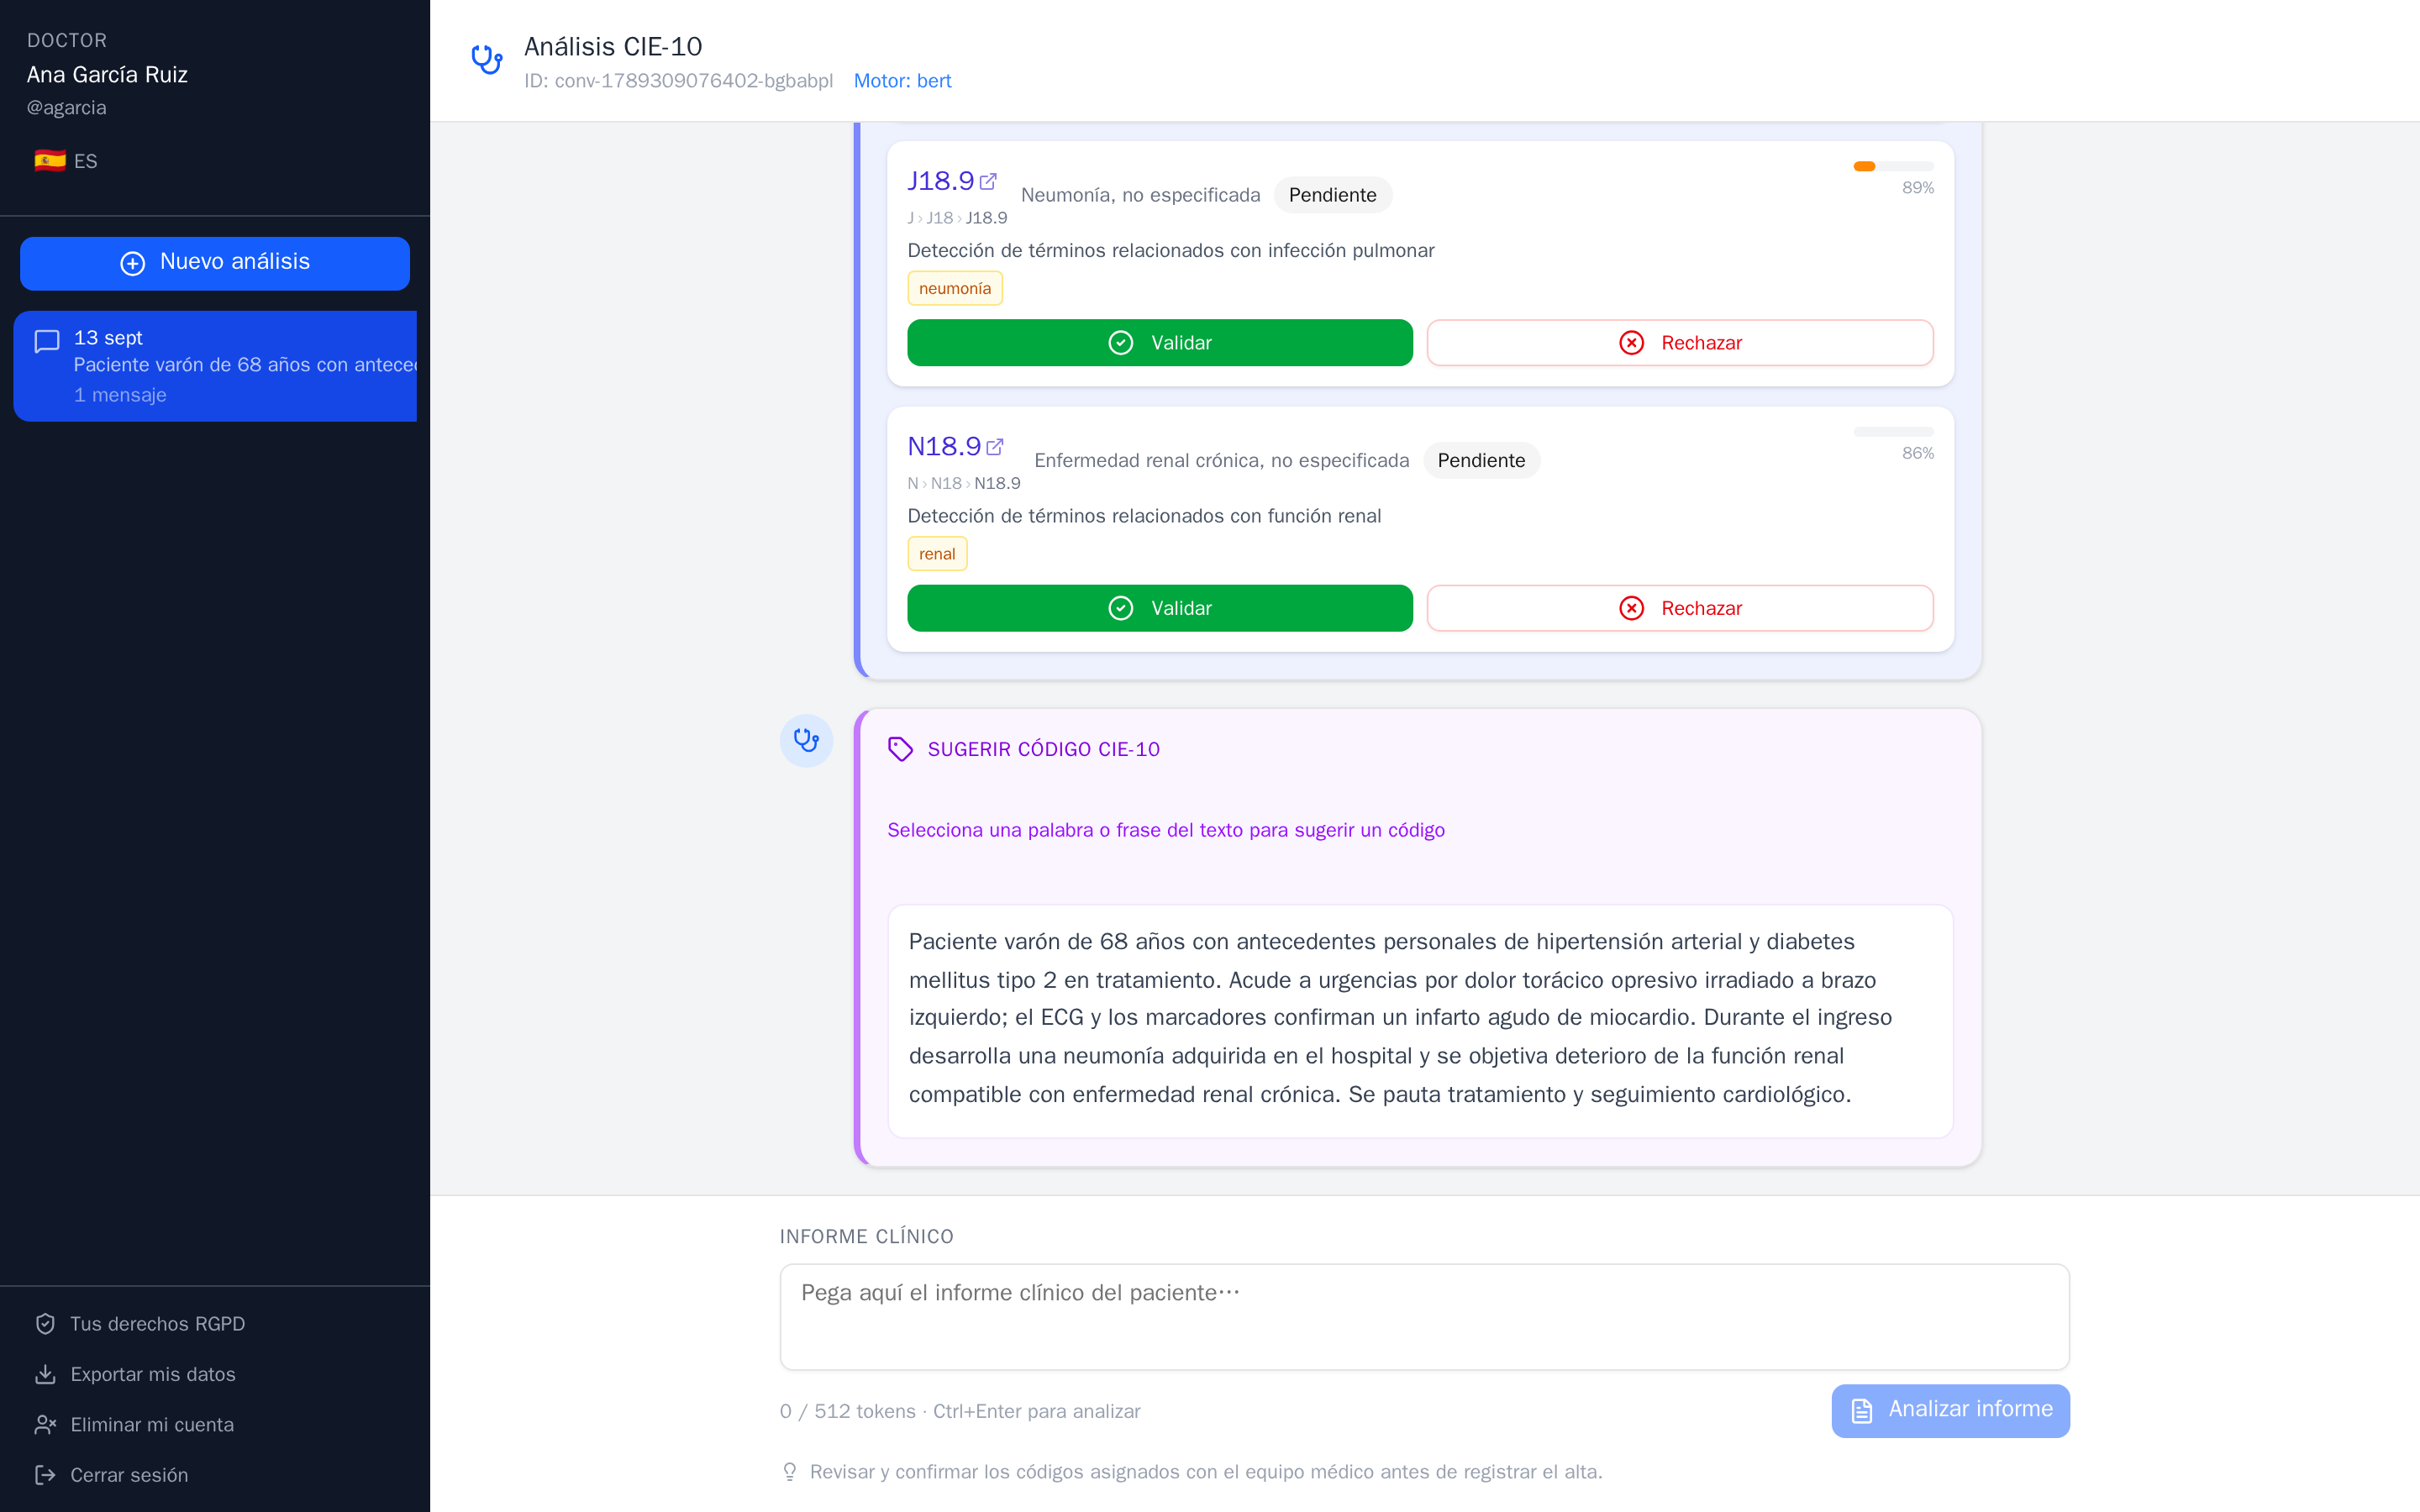
\includegraphics[width=0.8\textwidth, trim=920 0 360 130, clip]{figs/ui-analysis}
\caption{Área central de la interfaz web: tarjetas de códigos CIE-10 predichos, cada una con su nivel de confianza, los términos del informe que la motivan (\emph{chips} ámbar) y los controles de validación y rechazo, y el campo de entrada del informe. Se omite el panel lateral (historial y controles de sesión, incluidos los de RGPD), descrito en el texto.}
\label{fig:ui-analysis}
\end{figure}

\subsection{Requisitos}
\label{sec:requisitos}

A continuación se especifican los requisitos que debe cumplir el sistema, distinguiendo entre los funcionales, que describen qué debe hacer, y los no funcionales, que acotan cómo debe comportarse.

\subsubsection{Requisitos funcionales}

\begin{enumerate}[label=\textbf{RF\arabic*.}, leftmargin=*]
 \item \textbf{Entrada de datos:} Aceptar como entrada textos clínicos en español en formato libre, sin requerir marcado ni estructura predefinida.
 \item \textbf{Predicción de códigos:} Predecir uno o más códigos CIE-10-ES de diagnóstico para cada texto de entrada.
 \item \textbf{Puntuación de confianza:} Devolver una puntuación de confianza por cada código predicho, para priorizar la revisión humana de los casos de baja certeza.
 \item \textbf{Inferencia por lotes:} Admitir el procesamiento de múltiples textos de manera simultánea, devolviendo los resultados en el mismo orden que las entradas recibidas.
 \item \textbf{API REST:} Exponer las funcionalidades a través de una API REST documentada con al menos un endpoint de inferencia y uno de comprobación del estado del servicio.
\end{enumerate}

Los cinco anteriores acotan el motor de inteligencia artificial, que es el componente central. El sistema que se entrega, sin embargo, abarca los siete subobjetivos enumerados al principio del capítulo~\ref{cap:Objetivo}, de modo que los requisitos siguientes cubren las piezas restantes: el backend que orquesta el flujo, el módulo de resúmenes y la interfaz. Se enumeran aparte porque su verificación es de otra naturaleza, funcional y no métrica.

\begin{enumerate}[resume, label=\textbf{RF\arabic*.}, leftmargin=*]
 \item \textbf{Gestión de cuentas:} Permitir el alta de un usuario con verificación de la dirección de correo antes de conceder acceso, y autenticar las peticiones posteriores.
 \item \textbf{Orquestación del análisis:} Recibir un informe desde la interfaz, solicitar la predicción al motor y entregar los resultados de forma progresiva, sin que la parte más lenta del análisis retrase la aparición de los códigos.
 \item \textbf{Revisión de los códigos propuestos:} Permitir al codificador clínico validar o rechazar cada código, exigiendo un motivo en el rechazo, y conservar esas decisiones asociadas al análisis.
 \item \textbf{Resumen del informe:} Generar, mediante un modelo de lenguaje ejecutable en CPU, un resumen o paráfrasis del informe que se muestre junto a los códigos para agilizar la revisión.
 \item \textbf{Interfaz web:} Ofrecer una interfaz que permita enviar informes, seguir el análisis mientras se produce, consultar los términos que justifican cada código y recuperar los análisis anteriores.
\end{enumerate}

\subsubsection{Requisitos no funcionales}

\begin{enumerate}[label=\textbf{RNF\arabic*.}, leftmargin=*]
 \item \textbf{Rendimiento:} El sistema debe situarse dentro del rango de resultados de los sistemas participantes en el \emph{benchmark} CodiEsp~\cite{miranda2020}, que actúa como referencia, medido con la métrica oficial de la tarea (MAP por documento) sobre el mismo conjunto de prueba. Se considera cumplido si el sistema no queda por debajo del último de los sistemas participantes.
 \item \textbf{Latencia:} La propuesta de códigos debe completarse por debajo del segundo por informe en CPU de gama alta, de modo que el codificador clínico reciba los candidatos sin espera apreciable. La atribución de los términos que justifican cada código queda fuera de ese límite: es un orden de magnitud más cara, se sirve en una petición independiente y puede llegar después de los códigos, porque el usuario la consulta solo cuando despliega un código concreto.
 \item \textbf{Modularidad:} Los diferentes módulos del sistema deben tener interfaces bien definidas y ser sustituibles de forma independiente, de modo que, por ejemplo, el modelo base pueda cambiarse sin modificar el servicio de inferencia.
 \item \textbf{Trazabilidad:} El sistema debe registrar para cada predicción la versión del modelo empleada y el identificador del informe procesado, en línea con los principios de auditabilidad del Reglamento UE 2017/745~\cite{eu2017745} aplicable al software de apoyo a la decisión clínica.
 \item \textbf{Privacidad y protección de datos:} El tratamiento de los informes clínicos y de los datos de usuario debe ajustarse al Reglamento General de Protección de Datos (RGPD)~\cite{RGPD16}: minimización de datos, cifrado en tránsito y ejercicio de los derechos de supresión y portabilidad.
\end{enumerate}

\section{Diseño del sistema}

Esta sección describe el diseño del sistema de fuera hacia dentro: primero la arquitectura general de contenedores y sus interfaces, después el diseño del componente más crítico, el motor de inteligencia artificial (adquisición de datos, arquitectura del clasificador y proceso de entrenamiento), y por último el backend y el frontend que lo integran en un producto utilizable.

\subsection{Arquitectura general}

El sistema sigue una arquitectura orientada a servicios con cuatro capas bien diferenciadas: motor de inteligencia artificial, backend, frontend y capa de datos. Cada capa se despliega como un contenedor Docker independiente y se comunica con el resto a través de interfaces explícitas, lo que permite actualizar o sustituir cualquier componente sin afectar al resto del sistema.

El \textbf{frontend} (Next.js, React 19) se comunica con el \textbf{backend} (Elixir, Phoenix 1.8) mediante dos canales: una API REST para operaciones de autenticación y consulta, y un canal WebSocket para la recepción de tarjetas de análisis en tiempo real. El backend actúa como orquestador central: recibe los informes clínicos del usuario, los envía al \textbf{motor de IA} (Python, FastAPI) a través de una llamada HTTP síncrona, y retransmite las predicciones resultantes al cliente a medida que se generan. La \textbf{base de datos} PostgreSQL almacena tanto el registro de eventos inmutable del \emph{event store} como las proyecciones de lectura actualizadas por los proyectores del backend.

Dos decisiones arquitectónicas clave vertebran el diseño. Por un lado, el patrón CQRS/\emph{Event Sourcing} en el backend proporciona trazabilidad de las acciones clínicas sobre cada análisis. Por otro lado, el motor de IA se mantiene como servicio independiente, lo que permite actualizar el modelo BERT sin recompilar ni reiniciar el resto del sistema. Para describir la arquitectura en detalle se emplea el modelo C4~\cite{Brown22}. La topología completa de contenedores, puertos y variables de entorno se amplía en el Anexo~\ref{cap:AnexoB}; los contratos de comunicación entre servicios, en el Anexo~\ref{cap:AnexoC}; el esquema de base de datos, en el Anexo~\ref{cap:AnexoD}; y las decisiones de diseño que justifican las elecciones tecnológicas, en el Anexo~\ref{cap:AnexoE}.

\textbf{Nivel de contexto.} El sistema recibe informes clínicos en texto libre de parte del codificador clínico y devuelve propuestas de codificación CIE-10-ES. Se comunica con el portal eCIE-maps del Ministerio de Sanidad como fuente de datos externa (en la fase de adquisición de datos).

\textbf{Nivel de contenedores.} El sistema se compone de cuatro contenedores:

\begin{enumerate}
 \item \textbf{Frontend} (Next.js 16, TypeScript): interfaz web que el usuario utiliza para enviar informes y visualizar resultados. Se comunica con el backend mediante una API REST para autenticación y con un canal WebSocket para el intercambio de mensajes en tiempo real.
 \item \textbf{Backend} (Elixir 1.19, Phoenix 1.8): orquestador central del sistema. Gestiona la autenticación de usuarios, la persistencia de conversaciones mediante CQRS/Event Sourcing con la biblioteca Commanded y la comunicación con el motor de IA.
 \item \textbf{AI Engine} (Python, FastAPI): servicio de inferencia que carga el modelo BERT entrenado y expone un endpoint \texttt{POST /predict} que recibe un texto clínico y devuelve los códigos CIE-10-ES predichos con sus puntuaciones de confianza.
 \item \textbf{Base de datos} (PostgreSQL 18): almacena usuarios, conversaciones, tarjetas de análisis y el registro de eventos del sistema (event store de Commanded).
\end{enumerate}

\subsection{Diseño del motor de inteligencia artificial}

El motor de IA es el componente más crítico del sistema. Su diseño pasa por tres fases: adquisición de datos, entrenamiento del modelo y exposición del servicio de inferencia.

\subsubsection{Adquisición de datos}
\label{sec:adquisicion}

El sistema requiere dos fuentes de datos complementarias: el corpus de informes clínicos anotados (CodiEsp) y el catálogo oficial de códigos CIE-10-ES con sus descripciones en español. La Figura~\ref{fig:pipeline-datos} resume el flujo completo, desde la adquisición hasta el entrenamiento.

\begin{figure}[ht]
\centering
\resizebox{\textwidth}{!}{
\begin{tikzpicture}[
  every node/.style={font=\normalsize\sffamily},
  src/.style={draw=palered!80, fill=palered!10, thick, rectangle, rounded corners=3pt,
              minimum width=2.8cm, minimum height=1.1cm, align=center},
  csvn/.style={draw=black!60, fill=gray!10, thick, rectangle, rounded corners=3pt,
               minimum width=3.4cm, minimum height=1.1cm, align=center},
  proc/.style={draw=aquaESI!80, fill=aquaESI!15, thick, rectangle, rounded corners=3pt,
               minimum width=3.2cm, minimum height=1.3cm, align=center},
  fin/.style={draw=ocre!80, fill=ocre!15, thick, rectangle, rounded corners=3pt,
              minimum width=3.0cm, minimum height=1.3cm, align=center},
  arr/.style={->, >=Stealth, thick},
]
\node[src] (ecie) at (0,1.3) {eCIE-maps};
\node[src] (codi) at (0,-1.3) {CodiEsp};
\node[csvn] (ccsv) at (4.6,1.3) {\texttt{cie10-*.csv}};
\node[csvn] (dcsv) at (4.6,-1.3) {\texttt{codiesp\_*.csv}};
\node[proc] (pre) at (9.4,0) {Preprocesado y\\particiones};
\node[fin] (trn) at (13.8,0) {Entrenamiento};

\draw[arr] (ecie) -- (ccsv);
\draw[arr] (codi) -- (dcsv);
\draw[arr] (ccsv) -- (pre);
\draw[arr] (dcsv) -- (pre);
\draw[arr] (pre) -- (trn);
\end{tikzpicture}
}
\caption{Flujo de datos del sistema: adquisición de las dos fuentes (catálogo CIE-10-ES por \emph{scraping} de eCIE-maps y corpus CodiEsp), generación de los CSV, preprocesado al formato multilabel, partición en train/val/test y entrenamiento.}
\label{fig:pipeline-datos}
\end{figure}

\paragraph{Corpus CodiEsp.}
El corpus CodiEsp~\cite{miranda2020} fue creado en el contexto de la tarea compartida CodiEsp de CLEF eHealth 2020 y constituye un recurso público de referencia para la codificación automática de textos clínicos en español. Contiene 1.000 casos clínicos publicados, escritos en español y de diversas especialidades médicas, anotados manualmente por codificadores profesionales con los códigos CIE-10-ES correspondientes, distribuidos en tres particiones:

\begin{itemize}
 \item \textbf{Entrenamiento:} 500 documentos (50\,\%).
 \item \textbf{Validación:} 250 documentos (25\,\%).
 \item \textbf{Test:} 250 documentos (25\,\%).
\end{itemize}

La adquisición se realizó mediante el script \texttt{collect\_codiesp\_dataset.py}, que descarga los ficheros de diagnósticos (sufijo \texttt{\_D\_}), procedimientos (\texttt{\_P\_}) y la variante extendida con anotaciones a nivel de \emph{span} (\texttt{\_X\_}), normaliza la codificación de caracteres y genera los ficheros CSV empleados en las fases de entrenamiento y evaluación.

\paragraph{Catálogo CIE-10-ES mediante \emph{scraping} del portal eCIE-maps.}
El diccionario oficial CIE-10-ES no está disponible en ningún formato de descarga pública estructurada. La única fuente oficial es el portal eCIE-maps del Ministerio de Sanidad (\texttt{www.eciemaps.sanidad.gob.es}), que expone los datos a través de una API web no documentada. Para obtener el catálogo completo se analizó el tráfico de red del portal identificando el patrón de los \emph{endpoints} REST que sirven los datos en formato JSON, y se desarrollaron tres scripts de extracción:

\begin{itemize}
 \item \texttt{collect\_diagnoses.py}: itera sobre las 260 combinaciones letra–dígito del \emph{endpoint} de diagnósticos mediante peticiones asíncronas con \texttt{grequests}. Genera \texttt{cie10-es-diagnoses.csv} con \textbf{101.246 registros}.
 \item \texttt{collect\_procedures.py}: recorre la jerarquía de tres niveles de procedimientos (secciones, subsecciones y tablas). Genera \texttt{cie10-es-procedures.csv} con \textbf{78.496 registros}.
 \item \texttt{collect\_chemicals.py}: recorre las 27 letras del índice de fármacos. Genera \texttt{cie10-es-\allowbreak{}chemicals.csv} con \textbf{5.050 registros}.
\end{itemize}

Tres factores técnicos fueron determinantes para el éxito de la extracción: la simulación de cabeceras HTTP de navegador (\texttt{User-Agent}, \texttt{Accept}, \texttt{Referer}) para evitar respuestas 403, el paralelismo con reintentos automáticos para garantizar la integridad del catálogo, y el procesamiento por lotes para evitar el agotamiento de memoria en el volumen de procedimientos. Cada entrada incluye el código, la descripción en español y metadatos clínicos (restricciones de sexo, edad perinatal/pediátrica/materna/adulta, exención de POA y prohibición como diagnóstico principal).

\subsubsection{Análisis exploratorio de los datos}
\label{sec:analisis_datos}

Antes de diseñar el modelo se realizó un análisis estadístico exhaustivo de ambas fuentes, documentado en los notebooks \texttt{codiesp\_analisis\_estadistico.ipynb} y\linebreak \texttt{cie10\_analisis\_estadistico.ipynb}.

\paragraph{Longitud de los textos clínicos.}
Los informes tienen una longitud media de 2.317 caracteres (349 palabras) en el conjunto de entrenamiento, con desviación estándar de 1.097 caracteres y rango entre 556 y 7.466 caracteres. La distribución es aproximadamente log-normal. Aplicando el tokenizador de RigoBERTa-Clinical se comprobó que el \textbf{53,6\,\% de los documentos de entrenamiento supera los 512 tokens} (máximo: 1.888 tokens) y que el \textbf{100\,\% queda por debajo de 2.048 tokens}, con una distribución prácticamente idéntica en validación y prueba (58\,\% supera los 512 tokens en ambas). Aunque más de la mitad de los informes se trunca a 512 tokens, los experimentos con ventanas más largas (sección~\ref{sec:entrenamiento}) no mejoraron el resultado, lo que es compatible con que buena parte de la información diagnóstica se concentre en esos primeros 512 tokens, aunque no se midió directamente. Esos resultados fundamentan la elección de \texttt{max\_length}=512 y el descarte de la ventana deslizante (Figura~\ref{fig:tokens}).

\begin{figure}[ht]
\centering
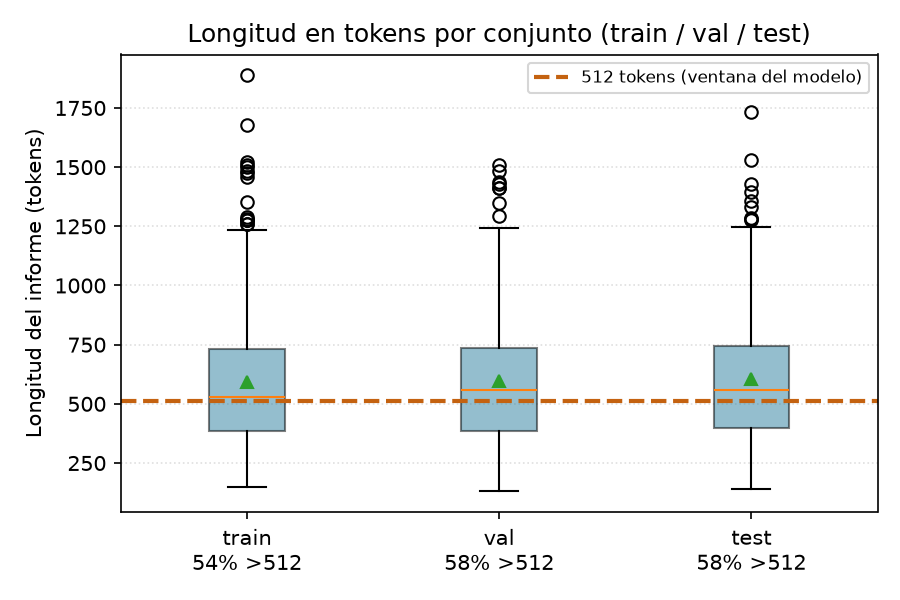
\includegraphics[width=0.72\textwidth]{figs/tfg_tokens}
\caption[Longitud de los informes en \emph{tokens} por conjunto (train/val/test)]{Longitud de los informes en \emph{tokens} por conjunto (train/val/test). Más de la mitad supera los 512 \emph{tokens} de la ventana del modelo (54\,\% en entrenamiento, 58\,\% en validación y prueba), pero la totalidad queda por debajo de 2.048. La distribución es homogénea entre los tres conjuntos.}
\label{fig:tokens}
\end{figure}

\paragraph{Distribución de etiquetas.}
Cada documento tiene una media de 11,3 códigos CIE-10-ES asignados (mediana: 10; máximo: 40; mínimo: 1). La correlación entre longitud del texto y número de etiquetas es de 0,56. La distribución de frecuencias sigue una ley de potencia: la mayoría de los 2.557 códigos únicos del corpus aparece en cinco o menos documentos. Esta distribución de cola larga motivó el uso de ponderación de clases en la función de pérdida (Figura~\ref{fig:longtail}).

\begin{figure}[ht]
\centering
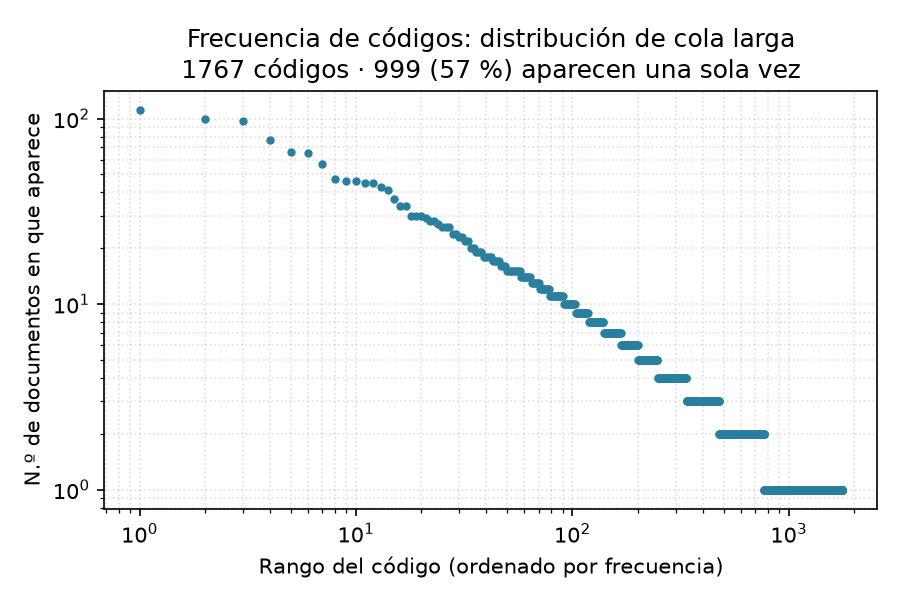
\includegraphics[width=0.72\textwidth]{figs/tfg_longtail}
\caption{Distribución de frecuencias de los códigos en el conjunto de entrenamiento (escala log-log): una minoría de códigos concentra la mayoría de las apariciones y más de la mitad aparece una sola vez, lo que motiva la ponderación de clases y el preentrenamiento.}
\label{fig:longtail}
\end{figure}

\paragraph{Solapamiento entre particiones.}
El coeficiente de Jaccard entre particiones se sitúa entre 0,31 y 0,33. El dato más relevante para la evaluación es que \textbf{el 38\,\% de los códigos distintos del conjunto de prueba (439 de 1.143, Tabla~\ref{tab:jaccard} del Anexo~\ref{cap:AnexoG}) no aparece en ningún documento de entrenamiento}, lo que impone un techo teórico al F1-macro independiente de la arquitectura elegida.

\paragraph{Características del catálogo CIE-10-ES.}
El catálogo contiene 101.246 entradas en 21 capítulos. Esta cifra supera los 68.069 códigos válidos de la CIE-10-ES~\cite{sanidad2016cie10} mencionados en la introducción porque el navegador eCIE-maps expone \emph{todos} los nodos del árbol jerárquico, incluidas las categorías de tres caracteres y las subcategorías intermedias, que no son códigos facturables finales; además, muchas entradas agrupan variantes o sinónimos de una misma descripción. Las categorías más representadas son R (síntomas y signos), S (traumatismos), T (envenenamientos) e I (enfermedades circulatorias). Esta distribución, unida a que solo una fracción de los códigos aparece en CodiEsp, explica que el espacio de clases del clasificador se limite a los 1.767 códigos completos (p.\,ej.\ \texttt{E11.9}) únicos del conjunto de entrenamiento, frente a los más de 100.000 del catálogo CIE-10-ES.

\paragraph{Brecha léxica entre catálogo oficial y lenguaje clínico real.}
El análisis lingüístico realizado con SpaCy (modelo \texttt{es\_core\_news\_lg}) sobre las descripciones del catálogo CIE-10-ES reveló que el vocabulario oficial emplea 10.874 lemas únicos, dominado por sustantivos técnicos (47,3\,\%) y adjetivos específicos (29,6\,\%). La validación cruzada de este vocabulario con los informes clínicos del corpus CodiEsp, documentada en el \emph{notebook} \texttt{cie10\_spacy\_word\_analysis.ipynb}, arrojó un resultado clínicamente significativo: \textbf{solo el 38,3\,\% de los lemas del catálogo oficial aparece en los textos de los informes clínicos del corpus}. Los 6.708 lemas restantes pertenecen a la nomenclatura estandarizada, pero no forman parte del lenguaje habitual con que se redactan los casos clínicos.

Esta brecha tiene una causa directa en la práctica clínica: el catálogo CIE-10 emplea denominaciones largas y normalizadas («infarto agudo de miocardio de cara anterior de transmisión transmural»), mientras que el médico redacta con abreviaturas frecuentes (\texttt{IAM}, \texttt{EPOC}, \texttt{HTA}, \texttt{DM2}), epónimos y expresiones propias del entorno hospitalario. El análisis identificó además un 44,4\,\% de lemas con especificidad máxima, asociados a un único código CIE-10, frente a términos de alta dispersión como «contacto», «fractura» o «especificado», que aparecen en miles de códigos diferentes. Esta estructura léxica justifica dos decisiones de diseño que se desarrollan en las secciones siguientes: (1) la elección de un \emph{encoder} preentrenado en texto clínico en español (RigoBERTa-Clinical), que ha aprendido a relacionar las expresiones del lenguaje médico real con las denominaciones de los diagnósticos sin depender de coincidencia léxica exacta; y (2) la expansión de abreviaturas clínicas implementada en el clasificador de diccionario, que normaliza expresiones habituales antes de la búsqueda en el catálogo. El análisis detallado del vocabulario se recoge en el Anexo~\ref{cap:AnexoG}.

\subsubsection{Métricas de evaluación}
\label{sec:metricas}

Las métricas se definen sobre el vocabulario $C$ del modelo (1.767 códigos) y un conjunto de documentos $D$. Para cada documento $d$ y código $c$, $y_{dc}\in\{0,1\}$ indica si $c$ figura en la anotación de referencia (\emph{gold}) y $\hat{y}_{dc}\in\{0,1\}$ si el sistema lo propone, es decir, si su probabilidad alcanza el umbral $\tau$. Por código, $TP_c=\sum_d y_{dc}\hat{y}_{dc}$, $FP_c=\sum_d (1-y_{dc})\hat{y}_{dc}$ y $FN_c=\sum_d y_{dc}(1-\hat{y}_{dc})$.

\paragraph{F1-micro y F1-macro.} El F1-micro agrupa todos los pares (documento, código), de modo que cada código pesa según su frecuencia:
\begin{equation}
P_{\mu}=\frac{\sum_c TP_c}{\sum_c (TP_c+FP_c)},\qquad R_{\mu}=\frac{\sum_c TP_c}{\sum_c (TP_c+FN_c)},\qquad F1_{\mu}=\frac{2\,P_{\mu}R_{\mu}}{P_{\mu}+R_{\mu}}.
\end{equation}
El F1-macro calcula el F1 de cada código y promedia sin ponderar:
\begin{equation}
F1_c=\frac{2\,TP_c}{2\,TP_c+FP_c+FN_c},\qquad F1_{M}=\frac{1}{|C|}\sum_{c\in C}F1_c,
\end{equation}
con $F1_c=0$ cuando el código no aparece ni en la referencia ni en las predicciones. Como el promedio recorre los 1.767 códigos, los poco frecuentes pesan tanto como los comunes y los que no tienen ejemplos en prueba cuentan como cero, lo que explica en parte la brecha entre F1-micro y F1-macro.

\paragraph{MAP por documento.} Para un documento $d$ se ordenan los códigos de $C$ por probabilidad decreciente (por puntuación fusionada en el modo fusionado) y se promedia la precisión en las posiciones donde aparece un código de la referencia:
\begin{equation}
AP_d=\frac{1}{n_d}\sum_{k=1}^{|C|}P_d@k\cdot rel_d(k),\qquad MAP=\frac{1}{|D'|}\sum_{d\in D'}AP_d,
\end{equation}
donde $P_d@k$ es la precisión de las $k$ primeras posiciones, $rel_d(k)=1$ si el código en la posición $k$ pertenece a la referencia y $n_d$ es el número de códigos de la referencia de $d$. A diferencia del F1, no depende del umbral: mide el orden, no la decisión. Con el mismo cálculo hay dos variantes, según el denominador. En el \emph{MAP estricto}, $n_d$ cuenta todos los códigos de la referencia, también los que están fuera del vocabulario del modelo, que nunca se pueden proponer y penalizan el resultado, y $D'$ son los documentos con al menos un código de referencia; es el comparable con el \emph{benchmark}. En el \emph{MAP alcanzable}, $n_d$ cuenta solo los códigos de la referencia que pertenecen al vocabulario y $D'$ los documentos con al menos uno; es una cota superior y no es comparable con otros sistemas. Las tres métricas se calculan en \texttt{ai\_engine/\allowbreak{}eval\_test.py} (\texttt{make ai-eval-test}).

\subsubsection{Selección del modelo base}

Se evaluaron diez modelos candidatos para la codificación del texto clínico. La comparativa, recogida en el Anexo~\ref{cap:AnexoA}, consideró rendimiento en CodiEsp, especialización en español médico, velocidad de inferencia y coste computacional de entrenamiento. Los modelos evaluados fueron:

\begin{itemize}
 \item \texttt{PlanTL-GOB-ES/roberta-base-biomedical-clinical-es} (RoBERTa-BSC, 125M parámetros), entrenado por el Barcelona Supercomputing Center sobre historias clínicas, informes radiológicos y notas médicas en español.
 \item \texttt{PlanTL-GOB-ES/roberta-large-bne} (355M parámetros), variante de mayor tamaño del mismo grupo (deprecado; referencia de escala).
 \item Longformer-BSC (\texttt{PlanTL-GOB-ES/\allowbreak{}longformer-base-4096-\allowbreak{}biomedical-clinical-es}, $\sim$130M parámetros, ventana de 4.096 tokens), variante del modelo clínico del Barcelona Supercomputing Center con atención dispersa para secuencias largas.
 \item \texttt{IIC/RigoBERTa-2.0} (arquitectura XLM-RoBERTa-large, $\sim$600M parámetros), versión de propósito general desarrollada por el Instituto de Ingeniería del Conocimiento sobre corpus español de gran escala.
 \item \texttt{IIC/RigoBERTa-Clinical} (XLM-RoBERTa-large, especialización clínica), variante de RigoBERTa entrenada sobre corpus médico en español por el Instituto de Ingeniería del Conocimiento; modelo seleccionado para el entrenamiento final en producción.
 \item \texttt{jhu-clsp/mmBERT-base} (mmBERT, arquitectura ModernBERT multilingüe), modelo con ventana de 8.192 tokens entrenado sobre 1800+ lenguas, desarrollado por el Centro de Procesamiento del Lenguaje y del Habla de la Universidad Johns Hopkins.
 \item \texttt{answerdotai/ModernBERT-base} (ModernBERT, 2024), arquitectura de última generación con Flash Attention y ventana de 8.192 tokens; obtuvo un F1-micro de 0{,}632 en pruebas de nivel~1.
 \item \texttt{dccuchile/bert-base-spanish-wwm-cased} (BETO, 110M parámetros), modelo de propósito general en español.
 \item \texttt{sentence-transformers/paraphrase-multilingual-MiniLM-L12-v2} (33M parámetros), orientado a la generación de embeddings.
 \item \texttt{distilbert-base-multilingual-cased} (66M parámetros), versión destilada multilingüe de BERT.
\end{itemize}

El modelo seleccionado como base fue \texttt{IIC/RigoBERTa-Clinical} para el entrenamiento final en producción, dado que combina la especialización en dominio clínico español con la mayor capacidad del grupo de modelos evaluados (XLM-RoBERTa-large, $\sim$600M parámetros) y obtuvo un F1-micro de 0{,}761 en la tarea de clasificación de capítulos, a dos puntos del mejor candidato y dentro de la dispersión entre ejecuciones. Para pruebas rápidas se usa \texttt{roberta-base} como alternativa más ligera.

\subsubsection{Arquitectura del clasificador}

El clasificador sigue una arquitectura plana (\emph{flat}) de clasificación multilabel. La entrada es el texto del informe clínico codificado por el tokenizador del modelo base; la salida es un vector de probabilidades de dimensión igual al número de códigos presentes en el corpus de entrenamiento (aproximadamente 1.767 códigos únicos en la partición de diagnósticos de CodiEsp).

Sobre el \emph{encoder} BERT se añade una cabeza de clasificación compuesta por una capa de \emph{dropout} (p\,=\,0,3 en producción) y una capa lineal que proyecta la representación del token \texttt{[CLS]} al espacio de códigos. La activación utilizada en inferencia es una sigmoide por código, de modo que cada predicción es independiente del resto y el modelo puede asignar simultáneamente cualquier subconjunto de códigos. Durante el entrenamiento se utiliza \emph{Binary Cross-Entropy} como función de pérdida. La planificación de la tasa de aprendizaje se determinó experimentalmente: la configuración de producción emplea un \emph{scheduler} de tipo \emph{plateau}, que resultó superior al \emph{cosine schedule with warmup} inicial (sección~\ref{sec:entrenamiento}).

La Figura~\ref{fig:arq-clasificador} resume esta arquitectura, del informe clínico a los códigos predichos.

\begin{figure}[ht]
\centering
\resizebox{\textwidth}{!}{% Arquitectura del clasificador plano multilabel CIE-10
% Uso: % Arquitectura del clasificador plano multilabel CIE-10
% Uso: % Arquitectura del clasificador plano multilabel CIE-10
% Uso: \input{figs/arq-clasificador} dentro de figure+\centering+\resizebox{\textwidth}{!}{...}
% Flujo: informe → tokenizador → encoder RigoBERTa-Clinical → [CLS] → dropout → lineal → sigmoide → umbral

\begin{tikzpicture}[
  every node/.style={font=\small\sffamily},
  io/.style={draw=palered!80, fill=palered!10, thick, rectangle, rounded corners=3pt,
             minimum width=2.1cm, minimum height=1.0cm, align=center},
  enc/.style={draw=aquaESI!80, fill=aquaESI!15, thick, rectangle, rounded corners=3pt,
              minimum width=3.0cm, minimum height=1.7cm, align=center},
  blk/.style={draw=gray!60, fill=gray!10, thick, rectangle, rounded corners=3pt,
              minimum width=1.9cm, minimum height=1.0cm, align=center},
  res/.style={draw=ocre!80, fill=ocre!18, thick, rectangle, rounded corners=3pt,
              minimum width=2.1cm, minimum height=1.0cm, align=center},
  arr/.style={->, >=Stealth, thick},
  node distance=0.65cm
]

\node[io] (inp) {Informe\\clínico};
\node[blk, right=of inp] (tok) {Tokenizador\\\scriptsize $\leq$512 tokens};
\node[enc, right=of tok] (enc) {\textbf{Encoder}\\RigoBERTa-Clinical\\\scriptsize XLM-R-large, 24 capas\\\scriptsize freeze=20 (4 entrenables)};
\node[blk, right=of enc] (cls) {token [CLS]\\\scriptsize 1024-d};
\node[blk, right=of cls] (drp) {Dropout\\\scriptsize 0,3};
\node[blk, right=of drp] (lin) {Capa lineal\\\scriptsize 1024$\to$1767};
\node[res, right=of lin] (sig) {Sigmoide\\\scriptsize por código};
\node[res, right=of sig] (thr) {Umbral 0,3\\\scriptsize $\to$ códigos};

\draw[arr] (inp) -- (tok);
\draw[arr] (tok) -- (enc);
\draw[arr] (enc) -- (cls);
\draw[arr] (cls) -- (drp);
\draw[arr] (drp) -- (lin);
\draw[arr] (lin) -- (sig);
\draw[arr] (sig) -- (thr);

% Nota: preentrenamiento débil antes del fine-tuning
\node[draw=turquesa!70, fill=turquesa!12, thick, rectangle, rounded corners=3pt,
      align=center, font=\scriptsize\sffamily, below=1.1cm of enc, text width=4.6cm]
      (pre) {\textbf{Preentrenamiento débil}\\descripciones CIE-10-ES + \emph{snippets} del task\_X\\$\rightarrow$ \emph{fine-tuning} sobre CodiEsp};
\draw[arr, turquesa!80, dashed] (pre) -- (enc);

\end{tikzpicture}
 dentro de figure+\centering+\resizebox{\textwidth}{!}{...}
% Flujo: informe → tokenizador → encoder RigoBERTa-Clinical → [CLS] → dropout → lineal → sigmoide → umbral

\begin{tikzpicture}[
  every node/.style={font=\small\sffamily},
  io/.style={draw=palered!80, fill=palered!10, thick, rectangle, rounded corners=3pt,
             minimum width=2.1cm, minimum height=1.0cm, align=center},
  enc/.style={draw=aquaESI!80, fill=aquaESI!15, thick, rectangle, rounded corners=3pt,
              minimum width=3.0cm, minimum height=1.7cm, align=center},
  blk/.style={draw=gray!60, fill=gray!10, thick, rectangle, rounded corners=3pt,
              minimum width=1.9cm, minimum height=1.0cm, align=center},
  res/.style={draw=ocre!80, fill=ocre!18, thick, rectangle, rounded corners=3pt,
              minimum width=2.1cm, minimum height=1.0cm, align=center},
  arr/.style={->, >=Stealth, thick},
  node distance=0.65cm
]

\node[io] (inp) {Informe\\clínico};
\node[blk, right=of inp] (tok) {Tokenizador\\\scriptsize $\leq$512 tokens};
\node[enc, right=of tok] (enc) {\textbf{Encoder}\\RigoBERTa-Clinical\\\scriptsize XLM-R-large, 24 capas\\\scriptsize freeze=20 (4 entrenables)};
\node[blk, right=of enc] (cls) {token [CLS]\\\scriptsize 1024-d};
\node[blk, right=of cls] (drp) {Dropout\\\scriptsize 0,3};
\node[blk, right=of drp] (lin) {Capa lineal\\\scriptsize 1024$\to$1767};
\node[res, right=of lin] (sig) {Sigmoide\\\scriptsize por código};
\node[res, right=of sig] (thr) {Umbral 0,3\\\scriptsize $\to$ códigos};

\draw[arr] (inp) -- (tok);
\draw[arr] (tok) -- (enc);
\draw[arr] (enc) -- (cls);
\draw[arr] (cls) -- (drp);
\draw[arr] (drp) -- (lin);
\draw[arr] (lin) -- (sig);
\draw[arr] (sig) -- (thr);

% Nota: preentrenamiento débil antes del fine-tuning
\node[draw=turquesa!70, fill=turquesa!12, thick, rectangle, rounded corners=3pt,
      align=center, font=\scriptsize\sffamily, below=1.1cm of enc, text width=4.6cm]
      (pre) {\textbf{Preentrenamiento débil}\\descripciones CIE-10-ES + \emph{snippets} del task\_X\\$\rightarrow$ \emph{fine-tuning} sobre CodiEsp};
\draw[arr, turquesa!80, dashed] (pre) -- (enc);

\end{tikzpicture}
 dentro de figure+\centering+\resizebox{\textwidth}{!}{...}
% Flujo: informe → tokenizador → encoder RigoBERTa-Clinical → [CLS] → dropout → lineal → sigmoide → umbral

\begin{tikzpicture}[
  every node/.style={font=\small\sffamily},
  io/.style={draw=palered!80, fill=palered!10, thick, rectangle, rounded corners=3pt,
             minimum width=2.1cm, minimum height=1.0cm, align=center},
  enc/.style={draw=aquaESI!80, fill=aquaESI!15, thick, rectangle, rounded corners=3pt,
              minimum width=3.0cm, minimum height=1.7cm, align=center},
  blk/.style={draw=gray!60, fill=gray!10, thick, rectangle, rounded corners=3pt,
              minimum width=1.9cm, minimum height=1.0cm, align=center},
  res/.style={draw=ocre!80, fill=ocre!18, thick, rectangle, rounded corners=3pt,
              minimum width=2.1cm, minimum height=1.0cm, align=center},
  arr/.style={->, >=Stealth, thick},
  node distance=0.65cm
]

\node[io] (inp) {Informe\\clínico};
\node[blk, right=of inp] (tok) {Tokenizador\\\scriptsize $\leq$512 tokens};
\node[enc, right=of tok] (enc) {\textbf{Encoder}\\RigoBERTa-Clinical\\\scriptsize XLM-R-large, 24 capas\\\scriptsize freeze=20 (4 entrenables)};
\node[blk, right=of enc] (cls) {token [CLS]\\\scriptsize 1024-d};
\node[blk, right=of cls] (drp) {Dropout\\\scriptsize 0,3};
\node[blk, right=of drp] (lin) {Capa lineal\\\scriptsize 1024$\to$1767};
\node[res, right=of lin] (sig) {Sigmoide\\\scriptsize por código};
\node[res, right=of sig] (thr) {Umbral 0,3\\\scriptsize $\to$ códigos};

\draw[arr] (inp) -- (tok);
\draw[arr] (tok) -- (enc);
\draw[arr] (enc) -- (cls);
\draw[arr] (cls) -- (drp);
\draw[arr] (drp) -- (lin);
\draw[arr] (lin) -- (sig);
\draw[arr] (sig) -- (thr);

% Nota: preentrenamiento débil antes del fine-tuning
\node[draw=turquesa!70, fill=turquesa!12, thick, rectangle, rounded corners=3pt,
      align=center, font=\scriptsize\sffamily, below=1.1cm of enc, text width=4.6cm]
      (pre) {\textbf{Preentrenamiento débil}\\descripciones CIE-10-ES + \emph{snippets} del task\_X\\$\rightarrow$ \emph{fine-tuning} sobre CodiEsp};
\draw[arr, turquesa!80, dashed] (pre) -- (enc);

\end{tikzpicture}
}
\caption{Arquitectura del clasificador plano multilabel: el \emph{encoder} RigoBERTa-Clinical (preentrenado de forma débil sobre el catálogo CIE-10-ES antes del \emph{fine-tuning}) proyecta la representación del token \texttt{[CLS]} sobre los 1.767 códigos mediante una cabeza lineal con activación sigmoide por código.}
\label{fig:arq-clasificador}
\end{figure}

La selección de los códigos predichos se realiza mediante un umbral sobre la probabilidad, 0,2 en la configuración de producción, seleccionado mediante barrido en validación (sección~\ref{sec:entrenamiento}); el servicio lo lee del fichero \texttt{config.json} generado durante el entrenamiento. El servicio devuelve como máximo los diez códigos de mayor probabilidad que superan el umbral (el límite está fijado en el código del servicio, no en \texttt{config.json}) y, si ninguno lo supera, la lista queda vacía.

\paragraph{FlashAttention~2: implementación eficiente del mecanismo de atención.}
El \emph{encoder} de RigoBERTa-Clinical utiliza FlashAttention~2~\cite{dao2023flashattention2} en lugar de la implementación estándar de auto-atención de PyTorch. FlashAttention~2 reordena el cómputo de la atención para reducir el consumo de memoria y acelerar cada paso sin alterar el resultado en aritmética exacta. Sobre la tarea de capítulos y la máquina de desarrollo (RTX 4080), la mediana por época baja de 11,9~s con la implementación \texttt{sdpa} de PyTorch a 9,9~s con FlashAttention~2, un 17\,\% menos. Conviene matizar esa última afirmación, porque el entrenamiento se realiza en \texttt{bfloat16}: el reordenamiento cambia el orden de acumulación y, con esa precisión, el resultado no es bit a bit idéntico. En cuanto al resultado, esa misma comprobación da 0,748 con \texttt{sdpa} frente a 0,757 y 0,764 con FlashAttention~2, una diferencia del mismo orden que la dispersión entre ejecuciones con la misma configuración, de modo que no cabe atribuirle un efecto sistemático.

Lo que sí tiene consecuencias es cómo se elige la implementación. Los cuadernos la seleccionaban en función de si la biblioteca estaba instalada en la imagen, lo que hacía que el mismo código diera resultados distintos en entornos distintos sin que nada lo indicara. Se fija ahora de forma explícita mediante el parámetro \texttt{ATTN\_IMPL} de la configuración de los cuadernos, que es condición necesaria para que una ejecución sea reproducible: una dependencia presente o ausente no debe decidir en silencio cómo se entrena el modelo.

\paragraph{Clasificador de diccionario (\texttt{baseline\_dict.py}).}
\label{sec:diccionario}
El motor de IA incluye un clasificador de diccionario que actúa como \textbf{complemento determinista} de RigoBERTa-Clinical, no como alternativa. Cumple tres funciones: sirve de \emph{baseline} de referencia para evaluar el valor añadido del modelo neuronal, actúa de \emph{fallback} cuando el modelo BERT no está disponible en producción, y puede combinarse con las predicciones neurales a través del parámetro \texttt{engine=\textquotedbl{}both\textquotedbl{}} del endpoint \texttt{POST /predict}, que devuelve las predicciones de cada motor de forma independiente con su campo identificador.

El clasificador opera mediante coincidencia de patrones lematizados sobre cinco fuentes de conocimiento complementarias:

\begin{enumerate}
 \item \textbf{Descripciones oficiales CIE-10-ES} (\emph{diagnoses}): cada código y sus variantes (separadas por \texttt{|} en el catálogo) se lematiza y se compila como expresión regular con delimitadores de palabra para evitar falsos positivos por subcadena.
 \item \textbf{Diccionario de procedimientos CIE-10-PCS} (\emph{procedures}): ídem sobre las descripciones de procedimientos, cuya co-ocurrencia con diagnósticos aporta señal correlada.
 \item \textbf{Diccionario de sustancias y fármacos} (\emph{chemicals}): nombres de fármacos y sustancias del catálogo CIE-10-MC.
 \item \textbf{Términos clínicos reales} (\emph{clinical}): fragmentos de texto extraídos de las anotaciones de explicabilidad del task\_X de CodiEsp (el texto literal que el anotador señaló como evidencia de cada código), expandidos con sinónimos léxicos mediante los word vectors de \texttt{es\_core\_news\_lg}. Esta fuente es \emph{semi-supervisada} porque usa anotaciones del conjunto de validación.
 \item \textbf{N-gramas discriminativos del corpus} (\emph{corpus}): secuencias de 3--5 palabras extraídas de las notas de entrenamiento, sin dígitos sueltos, con frecuencia mínima 3 y precisión mínima 0,75 respecto al bloque que las contiene, asignadas en exclusiva al bloque de mayor precisión para que un mismo n-grama no contamine varios códigos.
\end{enumerate}

Antes de cualquier comparación, el texto del informe se lematiza con \texttt{es\_dep\_news\_trf} (transformer contextual) y se expanden las abreviaturas clínicas más frecuentes (\texttt{HTA} → \emph{hipertensión arterial}, \texttt{IAM} → \emph{infarto agudo de miocardio}, \texttt{EPOC} → \emph{enfermedad pulmonar obstructiva crónica}, etc.) para ampliar la cobertura léxica con un riesgo bajo de introducir falsos positivos. Las cinco fuentes se pueden evaluar por separado para medir su aportación individual, pero \textbf{en producción el diccionario combina solo \emph{clinical} y \emph{corpus}}: un experimento controlado que añadió también \emph{diagnoses}, \emph{procedures} y \emph{chemicals} a la combinación resultó contraproducente pese a proceder de catálogos oficiales. La razón es la misma dispersión léxica descrita en el análisis de vocabulario (Anexo~\ref{cap:AnexoG}): muchos códigos solo tienen descripciones genéricas («contacto», «fractura», «especificado») que aparecen en miles de códigos distintos, y su inclusión inunda el diccionario de falsos positivos (de 12.723 a 546.304 patrones, con el F1-micro de prueba cayendo de 0,672 a 0,519 y el MAP de 0,461 a 0,308), así que se descartó para la combinación final.

El Algoritmo~\ref{alg:diccionario} resume cómo se predice con los patrones resultantes: un bloque se propone cuando al menos uno de sus patrones aparece en el texto lematizado, con la confianza del patrón más fiable que coincide, y se conservan hasta tres términos para poder explicar la predicción.

\begin{algorithm}[ht]
\DontPrintSemicolon
\caption{Clasificación por diccionario de bloques.}
\label{alg:diccionario}
\KwIn{informe $t$; para cada bloque $b$, patrones $\{(\pi_{b,i},\kappa_{b,i})\}$, con $\pi_{b,i}$ una frase lematizada y $\kappa_{b,i}$ su confianza según su procedencia}
\KwOut{lista de ternas (bloque, confianza, términos) ordenada por bloque}
$t' \leftarrow$ normalizar(lematizar(expandir\_abreviaturas($t$)))\;
$R \leftarrow \emptyset$\;
\ForEach{bloque $b$}{
  $H \leftarrow \{\, i : \pi_{b,i}$ aparece en $t'$ como secuencia de palabras completas$\,\}$\;
  \If{$H \neq \emptyset$}{
    ordenar $H$ por $\kappa_{b,i}$ decreciente\;
    $\kappa_b \leftarrow \kappa_{b,H_1}$\;
    añadir a $R$ la terna $(b,\ \kappa_b,\ \{\pi_{b,i} : i \in H_{1..3}\})$\;
  }
}
\Return{$R$ ordenado por bloque}\;
\end{algorithm}

Una primera versión de \emph{clinical}+\emph{corpus} sufría además de baja precisión por dos fuentes de ruido concretas: la expansión de sinónimos por word vectors capturaba variantes morfológicas sin relación semántica real (p.\,ej. «cloruro» → «tricloruro», «dolor» → «dolorcillo»), y los n-gramas del corpus, con un umbral de precisión laxo sobre solo 500 notas de entrenamiento, fijaban frases genéricas como patrón de un código («tumor de», «1,2 cm»). Se corrigió endureciendo ambos filtros (umbral de similitud de sinónimos de 0,65 a 0,80 con rechazo de subcadenas, y los parámetros de n-gramas del corpus recogidos en la enumeración anterior), lo que redujo el diccionario de 44.606 a 12.723 patrones ($-$71\,\%) eliminando las familias de ruido identificadas. Cada patrón guardado lleva además una \textbf{confianza según su procedencia} en vez del valor fijo 1,0 original: 0,95 para el término real anotado por CodiEsp, 0,6 para sus variantes por sinónimo, y la propia precisión estadística (0,75--1,0) para los n-gramas de \emph{corpus}; el código predicho hereda la confianza de su patrón más fuerte, y sus términos disparadores se listan de mayor a menor confianza, lo que permite comparar de forma más informativa con las probabilidades de RigoBERTa-Clinical en el modo \texttt{engine=\textquotedbl{}both\textquotedbl{}}. Un segundo experimento intentó corregir un caso marginal de la expansión de sinónimos: una discordancia de género gramatical dejaba sin generar un puñado de patrones («izquierda» y «izquierdo» no compartían entrada en el mapa de sinónimos). El arreglo, en teoría correcto, desbloqueó muchas más expansiones por sinónimo que resultaron ser ruido en la práctica y empeoró el resultado (F1-micro de prueba 0,672→0,637, MAP 0,461→0,419), por lo que también se revirtió. Ambos experimentos confirman la misma lección: con solo 500 notas de entrenamiento, ampliar la cobertura léxica sin más casi siempre pierde frente a la precisión, y ningún cambio se da por bueno sin medirlo contra el conjunto de prueba.

Evaluado sobre el conjunto de prueba de CodiEsp a nivel de bloque de 3 caracteres (la granularidad de este componente), el diccionario combinado \emph{clinical}+\emph{corpus} alcanza F1-micro~0,672 (precisión 0,638, \emph{recall} 0,709) y un MAP por documento de 0,461; el F1-macro (0,289) queda muy por debajo por los códigos de cola larga sin ningún patrón que los cubra, limitación estructural de construir el diccionario a partir de solo 500 notas. A diferencia de un diccionario construido a mano como el del equipo IAM-Burdeos, donde la alta precisión se debe a que cada término fue seleccionado manualmente por ser inequívoco, este sigue dependiendo de heurísticas automáticas de generación.

\paragraph{Comparación homogénea entre los dos motores.}
Las cifras anteriores no son directamente comparables con las del clasificador neuronal, que opera sobre códigos completos. Para poder contrastarlos se evaluó también RigoBERTa-Clinical a nivel de bloque de tres caracteres, agregando la probabilidad de cada bloque como el máximo de las probabilidades de los códigos que cuelgan de él. La Tabla~\ref{tab:motores} recoge el resultado sobre el mismo conjunto de prueba, la misma granularidad y las mismas métricas.

\begin{table}[h]
\centering
\small
\caption{Diccionario frente a clasificador neuronal, ambos a nivel de bloque de tres caracteres sobre el conjunto de prueba de CodiEsp (umbral global 0,2 para el modelo neuronal). Diccionario generado con \texttt{make ai-baseline-dict} (\texttt{ai\_engine/\allowbreak{}baseline\_dict.py}); la fila neuronal es el modelo servido, \texttt{zlpr-map}, ajuste fino de RigoBERTa-Clinical (Anexo~\ref{cap:AnexoH}), y sale de \texttt{make ai-eval-test} (\texttt{model/\allowbreak{}eval\_test.json}, clave \texttt{block\_level}).}
\label{tab:motores}
\begin{tabular}{lrrrr}
\hline
\textbf{Motor} & \textbf{P} & \textbf{R} & \textbf{F1-micro} & \textbf{MAP} \\
\hline
Diccionario (\emph{clinical}+\emph{corpus}) & 0{,}638 & 0{,}709 & \textbf{0{,}672} & 0{,}461 \\
RigoBERTa-Clinical, modelo servido (\texttt{zlpr-map}) & 0{,}611 & 0{,}462 & 0{,}526 & \textbf{0{,}567} \\
\hline
\end{tabular}
\end{table}

El resultado reproduce, dentro de este trabajo, el mismo patrón que separa a los dos primeros sistemas del \emph{benchmark} CodiEsp descrito en la introducción: el diccionario obtiene un F1 muy superior (+14{,}6\,pp) porque la coincidencia léxica exacta produce predicciones de alta precisión, mientras que el modelo neuronal ordena mejor (+10{,}6\,pp de MAP), que es la métrica oficial de la tarea. El equipo IAM lideró el F1 de 2020 con 0,687 y quedó en MAP por detrás de IXA-AAA; aquí ocurre lo mismo entre los dos motores del propio sistema. La lectura es que cada uno aporta algo distinto: el diccionario acierta con seguridad lo que reconoce y no propone nada fuera de su léxico, y el modelo neuronal cubre formulaciones no indexadas y sitúa mejor los códigos correctos en las primeras posiciones de la lista, que es lo que necesita un codificador clínico que revisa una propuesta ordenada. Por este motivo el clasificador de diccionario es un complemento, no un sustituto del modelo neuronal, y el \emph{endpoint} los expone de forma independiente mediante \texttt{engine=\textquotedbl{}both\textquotedbl{}}.

Un tercer motor, el \emph{modo fusionado} (\texttt{engine=\textquotedbl{}fused\textquotedbl{}}), combina ambos antes de ordenar (Algoritmo~\ref{alg:fusion}): suma al \emph{logit} de cada código una bonificación $\beta\,\kappa_b$, con $\kappa_b$ la confianza con que el diccionario ha detectado el bloque del código, y ordena y filtra con esa puntuación. La probabilidad que se muestra al usuario sigue siendo la del modelo. Los valores empleados son $\beta=6$ y un umbral de puntuación $\theta=2{,}1$, que el servicio lee de \texttt{config.json}.

\begin{algorithm}[ht]
\DontPrintSemicolon
\caption{Ordenación en el modo fusionado.}
\label{alg:fusion}
\KwIn{informe $x$; parámetros $\beta$ y $\theta$}
\KwOut{lista de códigos ordenada por puntuación}
$z \leftarrow$ logits del modelo sobre $x$\;
$\kappa \leftarrow$ confianza de cada bloque detectado por el diccionario (Algoritmo~\ref{alg:diccionario})\;
\ForEach{código $c$}{
  $s_c \leftarrow z_c + \beta\,\kappa_{\mathrm{bloque}(c)}$, con $\kappa_b = 0$ si el bloque no se detecta\;
}
$R \leftarrow \{\, c : s_c \geq \theta \,\}$\;
eliminar de $R$ los códigos que son prefijo de otro código de $R$\;
ordenar $R$ por $s_c$ decreciente\;
\Return{los diez primeros de $R$}\;
\end{algorithm}

\subsubsection{Proceso de entrenamiento experimental}
\label{sec:entrenamiento}

El proceso de entrenamiento se articuló en cuatro etapas, guiadas por los resultados en el conjunto de validación. El Anexo~\ref{cap:AnexoF} las desglosa por modelo y cuaderno en sus fases 0 a 5, que no coinciden una a una con estas etapas: las etapas 1 y 2 corresponden a las fases 0 a 4 de ese anexo (cuadernos sobre la clasificación de capítulos) y las etapas 3 y 4, a su fase 5 (entrenamiento sobre códigos). El entrenamiento no se detuvo tras cerrar esta fase: se siguen registrando ejecuciones en \texttt{training\_runs.csv} (78 a fecha de cierre de este documento, véase el recuento exacto y actualizado en el Anexo~\ref{cap:AnexoF}), lo que da trazabilidad al proceso. El Anexo~\ref{cap:AnexoF} recoge las curvas de aprendizaje más representativas y el Anexo~\ref{cap:AnexoH} los hiperparámetros y resultados finales.

\paragraph{Decisión arquitectural: clasificación en cascada vs. clasificador plano.}
La primera decisión de diseño fue la estrategia de clasificación. Se consideró una arquitectura de cascada en dos niveles: un clasificador de capítulos (19–21 clases) seguido de clasificadores especializados por capítulo, que reduciría el espacio de búsqueda en un 95\,\%. Para la implementación final se optó por un clasificador plano sobre los 1.767 códigos completos del espacio de entrenamiento, combinando la manejabilidad del segundo nivel con la compatibilidad con un único modelo de producción.

\paragraph{Etapa 1: exploración y descarte de modelos candidatos.}
De los diez modelos candidatos considerados (Anexo~\ref{cap:AnexoA}), cinco se llevaron a entrenamiento comparativo, atendiendo a la especialización en español médico, longitud de contexto y velocidad de inferencia. Para acelerar la comparación, todos los experimentos de esta fase se realizaron sobre la tarea de clasificación de \textbf{capítulos CIE-10} (21 clases), que actúa como aproximación de primer nivel: menos clases implican ciclos de entrenamiento más rápidos y resultados más interpretables, a la vez que el ranking relativo de modelos se transfiere bien a la tarea final. El clasificador de producción opera sobre los 1.767 códigos CIE-10 completos presentes en el conjunto de entrenamiento de CodiEsp. La Tabla~\ref{tab:modelos-capitulos} resume los resultados del clasificador de capítulos.

\begin{table}[ht]
\centering
\small
\caption[Comparativa de modelos en clasificación de capítulos (F1-micro en validación)]{Comparativa de modelos en clasificación de capítulos (F1-micro en validación). \texttt{bc} abrevia \texttt{biomedical-clinical}; prefijo \texttt{PlanTL-GOB-ES} omitido por espacio.}
\label{tab:modelos-capitulos}
\begin{tabular}{P{5.5cm}rllr}
\hline
\textbf{Modelo} & \textbf{Tokens} & \textbf{Idioma} & \textbf{Dominio} & \textbf{F1-micro} \\
\hline
PlanTL-GOB-ES/\allowbreak{}roberta-base-bc-es & 512 & ES & Biomédico & \textbf{0,780}$^{a}$ \\
IIC/RigoBERTa-Clinical & 512 & ES & Clínico & 0,761$^{a}$ \\
jhu-clsp/mmBERT-base & 1.200 & Multi & General & 0,707 \\
ModernBERT (answerAI) & 1.500 & EN & General & 0,632 \\
PlanTL-GOB-ES/\allowbreak{}longformer-base-4096-bc-es & 2.048 & ES & Biomédico & 0,416$^{b}$ \\
\hline
\end{tabular}

\smallskip\par\footnotesize Todas las cifras proceden de la reejecución de los cuadernos de \texttt{training/bert-classifier/} con \texttt{papermill}, con idéntico presupuesto (200 épocas, lote 8, umbral 0,2, paciencia 40) y quedan registradas en sus salidas: RoBERTa en el cuaderno 1, RigoBERTa en el 2, ModernBERT en el 4 y mmBERT en el 5. La ventana indicada es la efectivamente aplicada; RoBERTa y RigoBERTa no admiten más de 512 posiciones. $^{a}$~Media de dos ejecuciones (RoBERTa 0,771 y 0,788; RigoBERTa 0,757 y 0,764), que es la dispersión que cabe esperar sin semilla fijada. $^{b}$~Medido sobre los 809 bloques de tres caracteres, no sobre los 21 capítulos: es una tarea distinta y su F1 no es comparable con el resto de la columna.
\end{table}

El cribado descarta ModernBERT y mmBERT por razones que no dependen de la décima: ModernBERT está entrenado solo en inglés, y mmBERT, pese a ser multilingüe, carece de especialización en dominio clínico. Sus cifras confirman esa expectativa sin ser el motivo de la decisión. Entre los dos candidatos en español, RoBERTa-BSC y RigoBERTa-Clinical quedan a dos puntos, con una dispersión entre ejecuciones del mismo orden, de modo que esta tabla no establece un orden fiable entre ellos. Se optó por \texttt{IIC/RigoBERTa-Clinical} por ser el modelo más próximo al dominio del trabajo: está preentrenado sobre texto clínico en español, que es el tipo de documento que hay que codificar, y de esa cercanía se esperaba un mejor rendimiento en la tarea final. Conviene señalar que esa expectativa no llegó a contrastarse cara a cara: la fase de optimización se realizó íntegramente sobre RigoBERTa-Clinical (69 de las 78 ejecuciones registradas en \texttt{training\_runs.csv}, 58 de ellas sobre los 1.767 códigos) y no se entrenó RoBERTa-BSC sobre los 1.767 códigos, de modo que no existe una medición que compare ambos en la tarea real.

\paragraph{Etapa 2: clasificador de capítulos.}
RigoBERTa-Clinical alcanzó F1-micro = 0,761 en la tarea de capítulos, promediando dos ejecuciones. El principal hallazgo de esta fase fue la conveniencia de fijar un suelo a la tasa de aprendizaje (en torno a $10^{-5}$), que impide que el \emph{scheduler} la reduzca hasta valores en los que el modelo pierde capacidad de ajustar las clases minoritarias. Esta observación se incorporó después al uso del \emph{scheduler plateau} en la configuración final.

En esta fase se exploró además un mecanismo de autoajuste de los hiperparámetros del \emph{fine-tuning} mediante búsqueda bayesiana con Optuna~\cite{akiba2019optuna}. Ninguno de los ensayos completados superó la configuración manual de referencia, y la ejecución se detuvo antes de terminar: cada ensayo exige un entrenamiento completo del \emph{encoder}, de modo que el coste de la búsqueda no guardaba proporción con la mejora que cabía esperar. El código queda en el cuaderno correspondiente como constancia de la vía explorada.

\paragraph{Etapa 3: colapso trivial en el clasificador de códigos.}
La clasificación sobre 1.767 códigos presentó el reto del \textbf{colapso al mínimo local trivial}: con la función de pérdida binaria estándar, el modelo converge a predecir siempre cero (con 11 etiquetas positivas de media, el 99,4\,\% de las entradas son negativas). La solución fue la ponderación asimétrica por frecuencia inversa de clase:
\begin{equation}
w_c = \frac{N_{\text{total}} - N_c}{N_c + \varepsilon}
\end{equation}
donde $N_c$ es el número de ocurrencias del código $c$ en entrenamiento. El valor se acota con un máximo (\emph{cap}) de 10, el que emplea el modelo servido (Anexo~\ref{cap:AnexoH}) y 75 de las 78 ejecuciones registradas; los ensayos con 30 (dos ejecuciones) y con 3 (una) no lo mejoraron.

\paragraph{Etapa 4: optimización del clasificador plano.}
Las 42 ejecuciones sobre los 1.767 códigos anteriores a los experimentos de MAP (de las 58 registradas con ese espacio de salida) identificaron los factores de mayor impacto en F1-micro. Se adopta el F1-micro como métrica de optimización, en lugar del MAP utilizado como referencia en el benchmark CodiEsp original, porque el sistema emite una decisión binaria por código a un umbral fijo, y el rendimiento en ese punto de corte es más representativo que la calidad del \emph{ranking}. El F1-macro complementa al micro al ponderar todos los códigos por igual, siendo directamente sensible a la mejora en clases raras. La Tabla~\ref{tab:hitos} resume los hitos del proceso.

\begin{table}[h]
\centering
\caption{Hitos del proceso de optimización (F1-micro en validación, umbral global 0,3). Elaborada a partir de la columna \texttt{val\_f1\_micro} de \texttt{model/\allowbreak{}training\_runs.csv}, que \texttt{train.py} (\texttt{make ai-train-gpu}) amplía en cada ejecución; las tres primeras filas corresponden a la tarea de 809 bloques de tres caracteres, no a los 1.767 códigos.}
\label{tab:hitos}
\begin{tabular}{llr}
\hline
\textbf{Fecha} & \textbf{Cambio introducido} & \textbf{F1-micro} \\
\hline
2026-03-18 & Primera ejecución RigoBERTa (LR\,=\,$3\times10^{-5}$) & 0,320 \\
2026-03-19 & LR aumentado a $10^{-4}$ & 0,413 \\
2026-03-19 & Calibración de umbral (0,5 → 0,3) & 0,430 \\
2026-03-20 & Batch virtual 32 + preentrenamiento 10 épocas & 0,470 \\
2026-03-24 & \emph{LR schedule plateau} (vs. cosine) & 0,475 \\
2026-03-24 & \emph{Label smoothing} = 0,1 & 0,482 \\
2026-03-25 & Descongelado progresivo de capas & 0,484 \\
2026-03-26 & Paso~32b: configuración de referencia & 0,4888 \\
2026-05-30 & Paso~36: reejecución (fue el modelo de producción) & \textbf{0,4945} \\
\hline
\end{tabular}
\end{table}

Tres técnicas mostraron impacto relevante: (1) el \emph{preentrenamiento débil} sobre las descripciones CIE-10-ES y los fragmentos clínicos del task\_X de CodiEsp, que elevó el F1-micro de validación de 0,327 a 0,470, unos 14 puntos entre los pasos 20 y 23 (una sola ejecución por configuración); (2) el \emph{scheduler plateau}, que solo reduce el LR cuando el F1 se estanca en validación, evitando la convergencia prematura del schedule cosine; y (3) el \textbf{descarte de la ventana deslizante}, cuya fragmentación quizá rompe la coherencia clínica del informe (caída del F1-micro de validación de 0,484 a 0,412 en la única ejecución con ventana deslizante sobre 1.767 códigos, frente a la referencia del paso~30b). Los detalles de evaluación del modelo desplegado se recogen en el Anexo~\ref{cap:AnexoH}.

\paragraph{Determinación del límite de congelación y barrido de umbrales (pasos 11--18).}
La búsqueda del número óptimo de capas a congelar estableció que freeze=20 (solo las 4 capas superiores del \emph{encoder} más la cabeza clasificadora, $\sim$50\,M parámetros entrenables) fue el punto de equilibrio más estable de los ensayados con 500 muestras. Los intentos con freeze=16 (8 capas libres, $\sim$102\,M parámetros) colapsaron de forma sistemática con todas las tasas de aprendizaje probadas ($10^{-4}$, $3\times10^{-4}$, $5\times10^{-4}$). El ratio datos/parámetros ($\sim$$5\times10^{-6}$) es demasiado bajo para estabilizar el gradiente: el modelo tiene más grados de libertad que restricciones. Esta asimetría establece un \emph{techo duro} estructural (el número de capas entrenables está limitado por el tamaño del corpus, no por la capacidad del modelo) que condicionó el diseño del descongelado progresivo posterior. La combinación óptima dentro del régimen de freeze=20 fue LR\,=\,$10^{-4}$ (frente al $3\times10^{-5}$ inicial), que con pocos parámetros libres converge más rápido sin colapso.

Dos ejecuciones consecutivas de esta etapa, con umbrales de decisión de 0,3 y 0,2 (\texttt{20260319T102637Z} y \texttt{20260319T110051Z} en \texttt{training\_runs.csv}), dieron en validación F1-micro de 0,430 y 0,427 y F1-macro de 0,118 y 0,124. Es compatible con que el modelo, con BCE y pos\_weight, aprenda probabilidades sistemáticamente bajas para la mayoría de códigos, de modo que un umbral conservador de 0,5 descarta demasiados positivos reales, y con que un umbral más bajo favorezca la cobertura de códigos raros a costa de precisión; al no ser un barrido sobre un mismo modelo, no aísla el efecto del umbral. El umbral de producción se recalcula con un barrido sobre el mismo modelo cada vez que se promociona uno (Figura~\ref{fig:threshold}); en la configuración actualmente desplegada el óptimo de F1-micro cae en \textbf{0,2}.

\begin{figure}[ht]
\centering
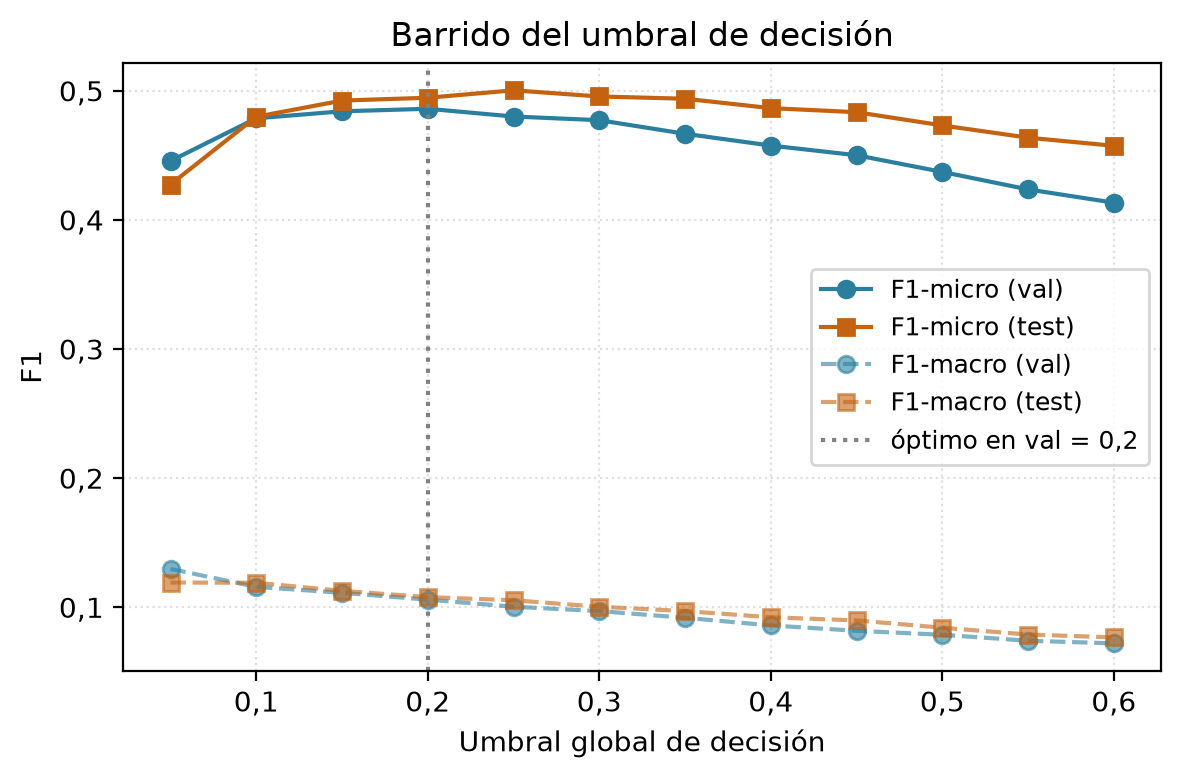
\includegraphics[width=0.72\textwidth]{figs/tfg_threshold}
\caption[Barrido del umbral global de decisión sobre validación y prueba]{Barrido del umbral global de decisión sobre validación y prueba. El F1-micro de validación se maximiza en 0,2 (umbral elegido); en prueba el máximo está en 0,25, a 0,6~pp del valor en 0,2, de modo que el umbral elegido sobre validación transfiere con una pérdida pequeña, aunque las curvas de precisión y \emph{recall} de ambas particiones difieren unos 4~pp en cada eje. El F1-macro decrece de forma monótona al subir el umbral.}
\label{fig:threshold}
\end{figure}

El mismo barrido, representado como curva precisión-\emph{recall} (Figura~\ref{fig:pr}), aporta dos lecturas que el barrido de F1 no deja ver. La primera es que la curva es prácticamente lineal en todo el rango útil: no hay codo ni punto de inflexión, de modo que cada punto de \emph{recall} ganado cuesta aproximadamente un punto de precisión y la elección del umbral es una decisión de política de uso, no un óptimo que la geometría de la curva imponga. El umbral 0,2 es simplemente el que maximiza el F1-micro, que pondera ambas por igual; para un sistema de ayuda a la codificación, donde el profesional revisa la propuesta y descartar un código erróneo cuesta menos que echar en falta uno correcto, un punto algo más orientado al \emph{recall} sería igualmente defendible. Se mantiene el óptimo de F1 por ser el criterio declarado de antemano y no ajustado a posteriori. La segunda lectura es que las curvas de validación y prueba se solapan casi por completo, lo que confirma que el umbral elegido sobre validación transfiere al conjunto de prueba y que la diferencia entre ambos conjuntos es de nivel, no de forma.

\begin{figure}[ht]
\centering
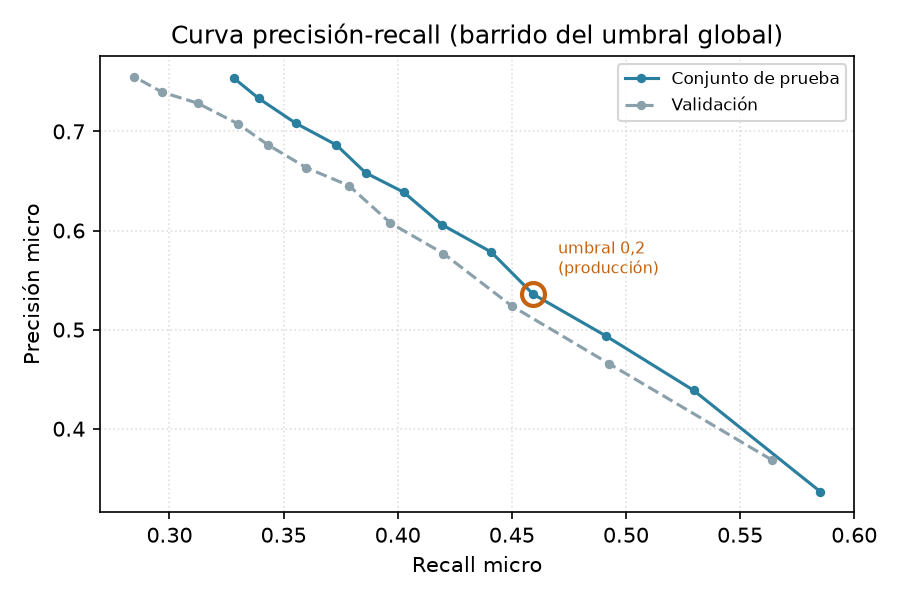
\includegraphics[width=0.72\textwidth]{figs/tfg_pr_curve}
\caption[Curva precisión-\emph{recall} del clasificador sobre validación y prueba, obtenida al barrer el umbral global de decisión]{Curva precisión-\emph{recall} del clasificador sobre validación y prueba, obtenida al barrer el umbral global de decisión. Se resalta el punto de operación de producción (umbral 0,2).}
\label{fig:pr}
\end{figure}

\paragraph{Modelos alternativos y granularidad de código (pasos 19--20).}
El modelo Longformer-BSC (\texttt{longformer-base-4096}, evaluado con una longitud de secuencia de 2.048 tokens) fue probado como alternativa para eliminar la truncación, que afecta a más de la mitad de los documentos (los que superan los 512 tokens). Pese a un recall superior (+5,8\,pp), el F1-micro cayó 1,4\,pp respecto a RigoBERTa-Clinical y el tiempo de entrenamiento aumentó 6,3× (70\,s/época frente a 11\,s). Una explicación posible, no contrastada, es que los diagnósticos clave se concentren en los primeros 512 tokens del informe y que el contexto adicional aporte más ruido que señal. RigoBERTa-Clinical con 512 tokens resultó la mejor opción de las ensayadas.

El paso al nivel de \emph{código completo} (1.767 clases, frente a 809 bloques de tres caracteres) conllevó una caída de 10\,pp en F1-micro: con 500 documentos de entrenamiento, la ratio datos/clase cae de $\sim$0,62 a $\sim$0,28. La degradación fue especialmente severa en F1-macro (0,118 → 0,050, $-$58\,\%), ya que códigos que aparecían 3 veces en train a nivel de bloque pasan a tener 1 aparición al subdividirse por subtipo. La elección de código completo para producción es correcta (el sistema clínico lo requiere), pero expone que el camino para recuperar esos 10\,pp pasa por aumentar los datos de entrenamiento, no por simplificar los objetivos.

\paragraph{Pre-entrenamiento débil (pasos 21--23).}
La escasez de datos para 1.767 clases motivó un pre-entrenamiento supervisado previo al \emph{fine-tuning} sobre CodiEsp. El mecanismo utiliza el catálogo CIE-10-ES como fuente de datos débilmente supervisados: para cada uno de los 1.767 códigos del vocabulario objetivo se extrae su descripción oficial (incluyendo variantes separadas por \texttt{|}) y se construye un par (descripción → código) que se usa como muestra de entrenamiento. De este modo el \emph{encoder} aprende a reconocer las \emph{keywords} clínicas de cada diagnóstico (terminología, siglas y variantes oficiales) antes de exponerse a las notas reales. En una ejecución, el pre-entrenamiento sobre las $\sim$3.200 variantes resultantes aportó +10,4\,pp de F1-micro (0,327 → 0,431). Añadir los 10.072 \emph{snippets} clínicos del task\_X de CodiEsp (fragmentos de texto real del médico anotados con su código) sumó 3,9\,pp adicionales (F1-micro=0,470) y una mejora del 51\,\% en F1-macro, porque esos \emph{snippets} enseñan la jerga real (\texttt{IAM}, \texttt{SCA}, \emph{dolor centrotorácico irradiado}) que el diccionario oficial no recoge. Un experimento de ablación con muestras negativas en el pre-entrenamiento resultó contraproducente; una explicación posible, no contrastada, es que el modelo aprenda a inhibir activaciones justo cuando necesita maximizar el reconocimiento de terminología.

\paragraph{Salvedad metodológica.} Los fragmentos del task\_X empleados en el pre-entrenamiento proceden de las particiones de entrenamiento \emph{y de validación} de CodiEsp, por lo que el modelo ha visto terminología anotada del conjunto sobre el que después se mide el F1-micro de validación. Es una contaminación parcial que conviene declarar: las cifras de validación deben leerse como una cota optimista. Su alcance está acotado por el propio conjunto de prueba, que no interviene en ninguna fase del entrenamiento: el F1-micro de prueba (0,4887) queda a solo 0,006 del de validación (0,4945), lo que indica que la ventaja obtenida es pequeña. Por este motivo, todas las cifras que se reportan como resultado final del trabajo se miden sobre el conjunto de prueba.

\paragraph{Experimentos con la función de pérdida (pasos 24 y 26).}
La Asymmetric Loss (ASL), que reduce o elimina la contribución de los negativos fáciles al gradiente, fue evaluada con $\gamma^- \in \{2, 4\}$. Con $\gamma^-=4$ el modelo colapsó al modo \emph{predecir todo} (F1-micro\,=\,0,375 frente a 0,470 de referencia). Con $\gamma^-=2$ el resultado fue prácticamente equivalente a BCE+pos\_weight ($-$1\,pp), sin beneficio neto. Subir el cap de pos\_weight de 10 a 30 no mejoró el resultado en las dos ejecuciones realizadas. La conclusión fue que el cuello de botella no es la ponderación de la función de pérdida sino la escasez de datos: con 999 códigos del vocabulario (el 56,5\,\%) vistos una sola vez y otros 568 con entre dos y cinco apariciones, es improbable que una ponderación compense la falta de ejemplos.

\paragraph{Técnicas de entrenamiento avanzadas y resultado final (pasos 28--32).}
Los últimos pasos introdujeron cuatro mejoras ortogonales que se acumularon en la configuración de producción:

\begin{itemize}
 \item \textbf{ReduceLROnPlateau} (paso 28b, +0,5\,pp): el \emph{schedule} coseno reducía el LR al 9\,\% del máximo en la época 60, cuando el modelo aún mejoraba. ReduceLROnPlateau mantiene el LR alto mientras hay mejora real y solo lo reduce cuando el F1 se estanca, permitiendo al modelo alcanzar su óptimo en la época 102.

 \item \textbf{Label smoothing one-sided} ($\varepsilon$=0,1, paso 29a, +0,68\,pp sobre 28b): suaviza los targets positivos de 1,0 a 0,9 pero mantiene los negativos en 0. El smoothing simétrico (0 → 0,05) colapsó el modelo al interaccionar con pos\_weight: el gradiente espurio de los negativos suavizados superó 13× al gradiente real de los positivos. La variante one-sided elimina esa interacción y reduce el sobreajuste de confianza en épocas tardías.

 \item \textbf{Descongelado progresivo} (paso 30b, unfreeze\_every=30, +0,23\,pp): a partir de la época 30 se descongelan 4 capas del \emph{encoder} cada 30 épocas con LR reducido ($10^{-5}$). Como hipótesis, no contrastada con una ablación por capas, las capas superiores son las más próximas a la tarea clínica y las que más necesitan adaptarse, mientras que las de bajo nivel (sintaxis, morfología) requerirían menos adaptación al dominio médico.

 \item \textbf{Regularizador de consistencia jerárquica} ($\lambda$=0,5, paso 32b, +0,46\,pp): CIE-10 tiene una estructura de árbol explícita (el código \texttt{J18.0} implica \texttt{J18}) que el clasificador plano ignora. Se añade el término $\ell_\text{hier} = \text{ReLU}(\text{logit}_\text{hijo} - \text{logit}_\text{padre})$ a la pérdida BCE con factor $\lambda=0{,}5$. La penalización es asimétrica: solo actúa cuando el hijo tiene logit superior al padre, sin interferir cuando el modelo ya es consistente. Con $\lambda=0{,}5$ se obtiene la mejor F1-micro del proceso; con $\lambda=0{,}1$ el mejor F1-macro por clase (+1,44\,pp respecto a la referencia), preferible cuando el objetivo es detección de códigos raros.
\end{itemize}

La Tabla~\ref{tab:progreso_pasos} recoge la evolución acumulada desde el clasificador plano sobre códigos completos hasta la configuración final, y la Figura~\ref{fig:waterfall} muestra la contribución de cada técnica al F1-micro resultante.

\begin{table}[h]
\centering
\small
\caption{Progreso acumulado del clasificador (F1 en validación CodiEsp, umbral global 0,3). Elaborada a partir de \texttt{model/\allowbreak{}training\_runs.csv} (ejecuciones de \texttt{make ai-train-gpu}) y del Anexo~\ref{cap:AnexoF}.}
\label{tab:progreso_pasos}
\begin{tabular}{P{1.0cm}P{7.0cm}rr}
\hline
\textbf{Paso} & \textbf{Técnica incorporada} & \textbf{F1-micro} & \textbf{F1-macro} \\
\hline
20 & Código completo sin preentrenamiento & 0,327 & 0,050 \\
21 & + Preentrenamiento sobre CIE-10 (3k descripciones) & 0,431 & 0,092 \\
23 & + Snippets clínicos task\_X (10k) & 0,470 & 0,139 \\
28b & + ReduceLROnPlateau & 0,475 & 0,116 \\
30b & + \emph{Label smoothing} + descongelado progresivo & 0,484 & 0,116 \\
\textbf{32b} & \textbf{+ Consistencia jerárquica ($\lambda$=0,5)} & \textbf{0,4888}$^\dagger$ & \textbf{0,120}$^\dagger$ \\
\hline
\end{tabular}
\smallskip\par\footnotesize $^\dagger$ Con umbral global de 0,3. Las cifras con umbrales por clase solo se conservan para la ejecución evaluada en profundidad (paso~36), y se recogen allí: aquí se omiten para no atribuir a 32b un dato que no se registró.
\end{table}

\begin{figure}[ht]
\centering
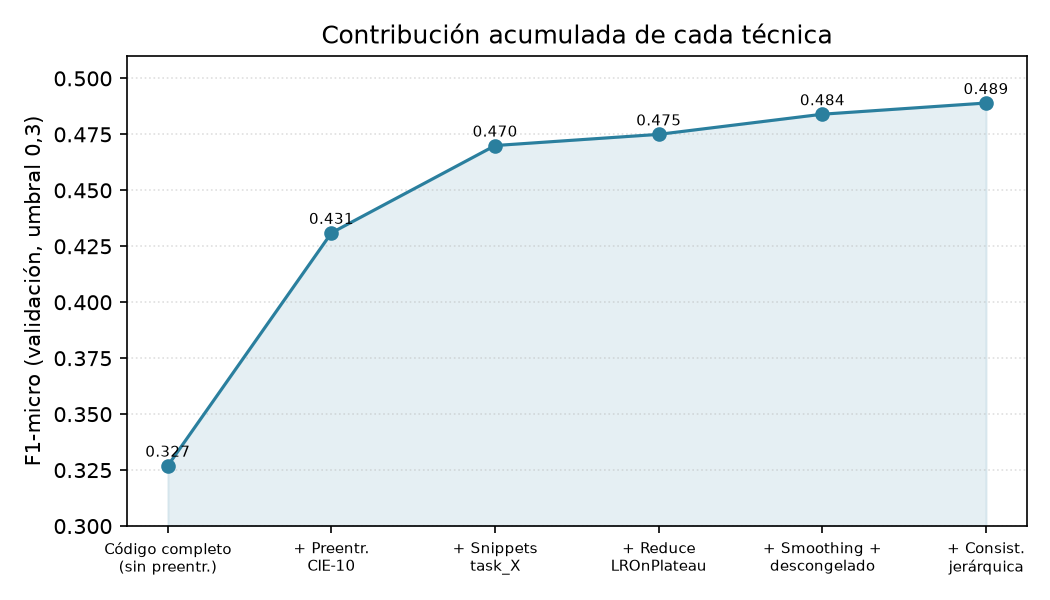
\includegraphics[width=0.78\textwidth]{figs/tfg_waterfall}
\caption{Contribución acumulada de cada técnica al F1-micro de validación (umbral 0,3), desde el clasificador plano inicial sobre códigos completos hasta la configuración final.}
\label{fig:waterfall}
\end{figure}

\subsubsection{Aumentación de datos mediante retrotraducción}
\label{sec:backtranslation}

El análisis de los experimentos anteriores reveló que la limitación principal no es la arquitectura ni la función de pérdida, sino la escasez de datos. El corpus de entrenamiento de CodiEsp contiene 500 documentos con una media de 11,28 etiquetas por nota, cubriendo los 1.767 códigos presentes en el corpus. La distribución de frecuencias es muy sesgada: el 56,5\,\% de los códigos aparece exactamente una vez y el 88,7\,\% no supera las cinco apariciones. Ninguna técnica de regularización puede compensar la escasez de señal de entrenamiento para las clases más raras.

La solución natural es generar datos sintéticos adicionales sin necesidad de anotación manual. La técnica empleada es la \textbf{retrotraducción} (\emph{back-translation})~\cite{sennrich2016improving}: cada nota clínica se traduce del español a un idioma pivote (inglés) y el resultado se vuelve a traducir al español. El texto final es semánticamente equivalente al original pero con diferente elección léxica y estructura sintáctica, actuando como una paráfrasis automática. Las etiquetas CIE-10 permanecen inalteradas porque la semántica clínica se conserva a través del pivote.

\paragraph{Generación y calidad del corpus aumentado.}
Con pivot EN se generaron 500 variantes retrotraducidas de las 500 notas originales, duplicando el corpus a 1000 documentos. La calidad de la traducción fue alta: el 99,2\,\% de las notas presentaron variación léxica efectiva, con un incremento medio de $+4{,}4$ palabras por nota (detalles en el Anexo~\ref{cap:AnexoL}). Para los 999 códigos que aparecían una sola vez, duplicar el número de ejemplos supone una mejora relativa del 100\,\% en la señal de entrenamiento. Las mejoras esperadas son:

\begin{itemize}
 \item \textbf{Códigos raros} (56,5\,\% del catálogo con una sola aparición): pasan a tener dos formulaciones distintas del mismo concepto, permitiendo al modelo aprender la invarianza semántica de cada código.
 \item \textbf{Robustez léxica}: el modelo deja de depender de formulaciones concretas del corpus original, ya que aprende la misma etiqueta asociada a expresiones diferentes.
 \item \textbf{F1-macro}: la métrica más sensible a las clases raras es la que más debería beneficiarse.
\end{itemize}

\paragraph{Implementación.}
Se diseñó el script \texttt{ai\_engine/augment.py} con dos \emph{backends} intercambiables: NLLB-200~\cite{costa-jussa2022nllb200} (modelo local de código abierto de Meta, sin coste externo) y Azure Translator (servicio en la nube con nivel gratuito de 2M caracteres/mes). El script incluye checkpoint incremental para reanudar traducciones interrumpidas. La integración con el flujo de entrenamiento se realiza mediante el target \texttt{make ai-augment} del \texttt{Makefile} y el parámetro \texttt{--train\_file} de \texttt{train.py}.

Se aplicaron tres pivotes independientes (EN, DE, FR), lo que cuadruplica el corpus de entrenamiento hasta 2.000 documentos. Las variantes se combinan mediante \texttt{ai\_engine/combine\_augmented.py} en un único CSV de entrenamiento. El proceso de configuración, los límites del servicio gratuito, las estadísticas de calidad por pivote y los comandos de uso se documentan en el Anexo~\ref{cap:AnexoL}.

\paragraph{Resultado del entrenamiento con datos aumentados.}
El entrenamiento con el corpus 4× se detuvo por \emph{early stop} en la época~51, antes de agotar el margen de épocas previsto. El resultado fue un F1-micro de \textbf{0,4668}, inferior al 0,4888 de referencia ($-0{,}022$). La causa más probable, que no se aisló con un experimento de control, es un desajuste en el \emph{schedule} de entrenamiento: con 2.000 documentos el número de pasos por época pasa de 63 a 250 (4×), pero el parámetro \texttt{UNFREEZE\_EVERY=30} no fue reescalado. Esto provoca que el primer descongelado de capas del \emph{encoder} ocurra tras 7500 pasos (frente a los 1890 del experimento de referencia), y es posible que el modelo converja en el régimen de \emph{freeze} total antes de que la señal de las capas superiores pueda aprovecharse, lo que explicaría el \emph{early~stop} en la época 51.

La hipótesis de trabajo es que al escalar el corpus conviene reescalar los hitos de unfreezing por la inversa del factor de datos: $\texttt{UNFREEZE\_EVERY} = \lceil 30 / 4 \rceil = 8$ para mantener el mismo número de pasos entre descongelados.

Durante el mismo experimento se observó además que el pre-entrenamiento estaba sobreajustado: la pérdida de \emph{pretrain} cae de 0,76 en el primer paso a 0,0038 al final de la época~1 y llega a 0,0008 en la época~6, esencialmente cero. Con la pérdida de \emph{pretrain} prácticamente nulo desde la época~6, las épocas 7--10 aparentaban ser prescindibles: no aportan señal nueva a la función de pérdida. El experimento de corrección (\emph{paso~33b}) aplica dos ajustes simultáneos: \texttt{UNFREEZE\_EVERY=8} y \texttt{PRETRAIN\_EPOCHS=3}, con la hipótesis de ahorrar $\sim$28~minutos de pre-entrenamiento y partir de una inicialización menos sobreajustada.

\paragraph{Pasos 33 a 35: qué se intentó y qué se aprendió.}
Tras fijar la configuración de referencia (32b, F1-micro~0,4888) se ensayaron tres vías para superarla: entrenar sobre el corpus aumentado por retrotraducción, aumentar el \emph{batch} efectivo a 64 mediante acumulación de gradiente, y acortar el preentrenamiento a 3 épocas dando a cambio más margen de entrenamiento. Ninguna la superó, y la Tabla~\ref{tab:paso35} recoge las cuatro variantes del paso~35 frente a la referencia. El desarrollo completo de cada ejecución, con sus cifras por época, está en el Anexo~\ref{cap:AnexoF}.

Las tres dejan una lección transferible, que es lo que justifica haberlas intentado:

\begin{itemize}
 \item \textbf{Entrenar con texto retraducido y validar con texto original puede abrir una brecha de distribución.} Una explicación plausible, no contrastada con un experimento de control, es que el modelo aprenda construcciones sintácticas características de la retraducción que el conjunto de validación, en español original, penaliza. Los datos sintéticos añaden variedad léxica, pero en estos experimentos no mejoraron el resultado.
 \item \textbf{Los hiperparámetros de calendario parecen depender del tamaño del corpus.} Con 500 documentos y \emph{batch}~8 hay 63 mini-lotes por época, de modo que acumular 8 deja solo 7 actualizaciones del optimizador por época frente a las 15 de la referencia. Con esa cadencia el \emph{scheduler} apenas recibe señal y el descongelado progresivo opera con gradientes menos informativos. \texttt{GRAD\_ACCUM}, \texttt{UNFREEZE\_EVERY} y \texttt{PATIENCE} fijan una cadencia por época y hay que recalibrarlos cada vez que cambia el número de muestras.
 \item \textbf{Que la pérdida de preentrenamiento llegue a cero no significa que esas épocas sobren.} Recortarlas de 10 a 3 costó 0,025 de F1-micro con todo lo demás idéntico, y restaurarlas recuperó el mismo valor de la referencia (con una sola ejecución por variante). La saturación aparente de la pérdida podría no ser sobreajuste evitable, sino convergencia gradual de las representaciones.
\end{itemize}

\begin{table}[h]
\centering
\small
\caption{Resumen del paso~35: comparativa de variantes frente a la ejecución de referencia 32b (F1 con umbral global 0,3). Cada F1 y su mejor época salen del historial por época de la ejecución (\texttt{model/\allowbreak{}training\_history\_*.json}, Anexo~\ref{cap:AnexoF}); \texttt{training\_runs.csv} registra 0,4651 para 35a y 0,4785 para 35d al reevaluar el \emph{checkpoint} guardado.}
\label{tab:paso35}
\begin{tabular}{llrrr}
\hline
\textbf{Ejec.} & \textbf{Corpus} & \textbf{F1-micro} & \textbf{F1-macro} & \textbf{Mejor época} \\
\hline
\textbf{32b (referencia)} & \textbf{500 docs originales} & \textbf{0,4888} & \textbf{0,1196} & \textbf{135} \\
35a & 500 docs, pretrain=3 & 0,4643 & 0,0990 & n/d \\
35b & 2000 docs (BT), pretrain=3 & 0,4569 & n/d & n/d \\
35c & 500 docs, pretrain=10 & 0,4888 & 0,1110 & 124 \\
35d & 2000 docs (BT), pretrain=10 & 0,4766 & 0,1140 & 29 \\
\hline
\end{tabular}
\end{table}

El artefacto de referencia de la selección de hiperparámetros es la ejecución del \textbf{paso~36} (el modelo que se sirvió hasta su sustitución por \texttt{zlpr-map}, descrita en el Anexo~\ref{cap:AnexoH}; las cifras y el umbral de 0,3 de este párrafo son los del paso~36, no los del modelo desplegado ahora), que reproduce la configuración de 32b sin modificar ningún hiperparámetro. Fue en su momento la mejor ejecución por F1-micro de validación, si bien su ventaja sobre 32b ($+0{,}006$) queda dentro del intervalo de variabilidad estocástica ($\pm 0{,}01$) discutido más adelante: se elige por ser el artefacto entrenado más reciente con esa configuración, no por una superioridad estadísticamente significativa. Sobre validación obtiene F1-micro~0,4945 y F1-macro~0,119 con umbral global de 0,3, el óptimo del barrido de umbrales, y sobre el conjunto de prueba F1-micro~0,4887 y F1-macro~0,109. Los umbrales por clase optimizados sobre validación elevan el F1-micro de validación a 0,551, pero \emph{no generalizan}: sobre el conjunto de prueba caen a 0,468, por debajo del umbral global, por lo que la configuración de producción emplea el umbral global. Corpus: 500 documentos originales, \texttt{PRETRAIN\_EPOCHS=10}. Esta ejecución, \texttt{classifier\_20260530T030233Z\_f1=0.4945.pt}, está publicada en HuggingFace\footnote{\url{https://huggingface.co/dmartingarcia/cie10-rigoberta-classifier}}; los detalles de evaluación se recogen en el Anexo~\ref{cap:AnexoH}. El entrenamiento no se detiene en este punto: la \textbf{política de despliegue} consiste en sustituir el artefacto de producción por el mejor modelo disponible tras confirmar sus cifras en el conjunto de prueba, no solo en validación (una F1-micro de validación más alta no basta si no se sostiene en prueba, como documenta la sección~\ref{sec:anexoH-candidatos}), sin necesidad de modificar código, únicamente actualizando \texttt{ai\_engine/model/config.json}. El Anexo~\ref{cap:AnexoF} recoge la tabla completa de ejecuciones con sus valores de F1-micro y MAP, y debe consultarse para conocer cuál es la configuración vigente en cualquier instante posterior al cierre de este documento; las vías de mejora restantes se recogen en la sección de trabajos futuros de las conclusiones.

\paragraph{La pérdida de ordenación del modelo servido.} El modelo que sirve el sistema, \texttt{zlpr-map} (ejecución \texttt{20260921T091919Z}), parte de la configuración del paso~36 y modifica dos elementos, ambos solo en el entrenamiento y sin coste de inferencia. El primero es un término de ordenación ZLPR~\cite{su2022zlpr}, con peso 0,1, que se suma a la entropía cruzada: penaliza que un código incorrecto de un informe quede por encima de uno correcto del mismo informe, que es lo que mide el MAP, sin exigir un valor absoluto de probabilidad. El segundo es elegir el \emph{checkpoint} por MAP de validación en lugar de por F1-micro, porque bajo entropía cruzada el MAP resultaba poco informativo y con el nuevo término vuelve a serlo. Con cuatro semillas, el MAP medio de prueba pasa de 0,4359 (cinco réplicas de control) a 0,4466, una diferencia de $+1{,}08$~pp (prueba $t$ de Welch, $p=0{,}045$) que es evidencia moderada y no concluyente. El modelo desplegado, de ese grupo, obtiene MAP 0,454 y F1-micro 0,495 frente a 0,437 y 0,488 del paso~36 (Anexo~\ref{cap:AnexoF}, sección~\ref{sec:anexoF-alineacion}, y Tabla~\ref{tab:candidatos} del Anexo~\ref{cap:AnexoH}).

La Tabla~\ref{tab:codiesp-comparativa} sitúa el modelo en el contexto del \emph{benchmark} CodiEsp-D 2020, la tarea compartida de referencia para codificación automática de diagnósticos clínicos en español~\cite{miranda2020}. El MAP de este trabajo se calcula sobre el mismo conjunto de prueba que emplearon los equipos participantes, por lo que la comparación es homogénea. El sistema se compara en sus dos configuraciones ejecutables. En la configuración por defecto, con el clasificador solo, obtiene un MAP de 0,454, que lo sitúa en el penúltimo lugar de la tabla, por delante únicamente de IMS. En \textbf{modo fusionado}, combinando el clasificador con el diccionario en un único \emph{ranking}, alcanza \textbf{0,554 y pasa a la segunda posición}, por delante de todos los demás sistemas de la tabla, incluidos los diccionarios construidos a mano y los basados en \emph{transformers}, y solo por detrás de IXA-AAA (XGBoost con BERT multilingüe). La diferencia entre ambas filas, diez puntos de MAP, es el resultado más relevante de este trabajo: no procede de un modelo mejor sino, probablemente, de combinar dos fuentes de evidencia que fallan en sitios distintos. Una salvedad: $\beta$ y el umbral se eligen sobre validación, pero el diccionario incorpora anotaciones del conjunto de validación (fuente \emph{clinical}), de modo que el ajuste en validación es optimista; la cifra de prueba no está contaminada, porque el diccionario nunca usa ese conjunto. Restringido al vocabulario de 1.767 códigos que el modelo puede predecir, el MAP de la configuración por defecto asciende a 0,555, pero esa cifra no es comparable con el resto de sistemas, que podían proponer cualquier código del catálogo. Las cifras de prueba del modelo servido citadas en este capítulo proceden del guion de evaluación en precisión completa (\texttt{eval\_test.py}), salvo la del modo fusionado (\texttt{motores\_eval.py}); los experimentos del Anexo~\ref{cap:AnexoF} emplean una pasada en precisión reducida que permite comparar muchos modelos entre sí en una sola ejecución y que sitúa este mismo modelo en 0{,}4535. La diferencia, de 0{,}04~pp, no afecta a ninguna conclusión, pero conviene no mezclar ambas procedencias al citar cifras.

Conviene cuantificar esa restricción antes de leer las cifras de \emph{recall}. De los 2.842 pares documento-código del \emph{gold} de prueba, 497 (el 17,5\,\%) corresponden a códigos ausentes del vocabulario de entrenamiento: ninguna arquitectura con este espacio de salida puede acertarlos. El \textbf{techo de recall} queda por tanto en 0,825. Hay que precisar sobre qué \emph{gold} se calculan la precisión, el \emph{recall} y el F1 de este trabajo: \texttt{eval\_test.py} los mide sobre los 2.345 pares alcanzables, de modo que el \emph{recall} de 0,459 es el del \emph{gold} alcanzable. Sobre el \emph{gold} completo de 2.842 pares, que es el que usan los equipos del \emph{benchmark}, los mismos 1.077 aciertos dan un \emph{recall} de 0,379 y un F1-micro de 0,444 (precisión 0,536). El MAP estricto sí penaliza los códigos inalcanzables y no se ve afectado. La diferencia entre ambas lecturas es la restricción estructural descrita en el análisis exploratorio (sección~\ref{sec:analisis_datos}), y es la razón por la que la vía de mejora pasa por ampliar el corpus anotado y no por cambiar de arquitectura.

\paragraph{De qué depende realmente el rendimiento.}
El análisis exploratorio mostró que la distribución de códigos sigue una ley de potencia; lo que no mostraba es cuánto cuesta eso en rendimiento. Agrupando los 1.767 códigos del vocabulario por su número de apariciones en el corpus de entrenamiento y midiendo cada grupo por separado sobre el conjunto de prueba se obtiene la relación de la Figura~\ref{fig:freq}, que es monótona y muy pronunciada: los 999 códigos vistos una sola vez alcanzan un F1-micro de 0,122, los vistos entre dos y cinco veces 0,328, y los 33 códigos con más de veinte apariciones llegan a 0,671. Esos 33 códigos, el 1,9\,\% del vocabulario, concentran 671 de los 2.345 pares alcanzables del \emph{gold} de prueba.

Una lectura posible es que el rendimiento por código depende sobre todo de cuántas veces lo ha visto el modelo. Es la misma tendencia que sugería la brecha entre F1-micro y F1-macro, medida ahora directamente: el F1-micro global de 0,495 es el promedio ponderado de un modelo que rinde razonablemente sobre el puñado de códigos frecuentes y que apenas reconoce la cola larga. Los cambios de arquitectura y de hiperparámetros de los pasos 24 a 35 no movieron el F1 más allá de la variabilidad entre ejecuciones (en torno a $\pm 0{,}01$), mientras que lo que sí elevó el MAP sin datos nuevos fue la pérdida de ordenación (aproximadamente $+1$~pp) y la fusión con el diccionario (unos 10~pp). Con los datos disponibles, ampliar el corpus anotado parece la vía con más recorrido para la cola larga, aunque no necesariamente la única; y la relación entre frecuencia y F1 puede estar mezclada con la dificultad propia de cada código, algo que esta medición no permite separar.

\begin{figure}[ht]
\centering
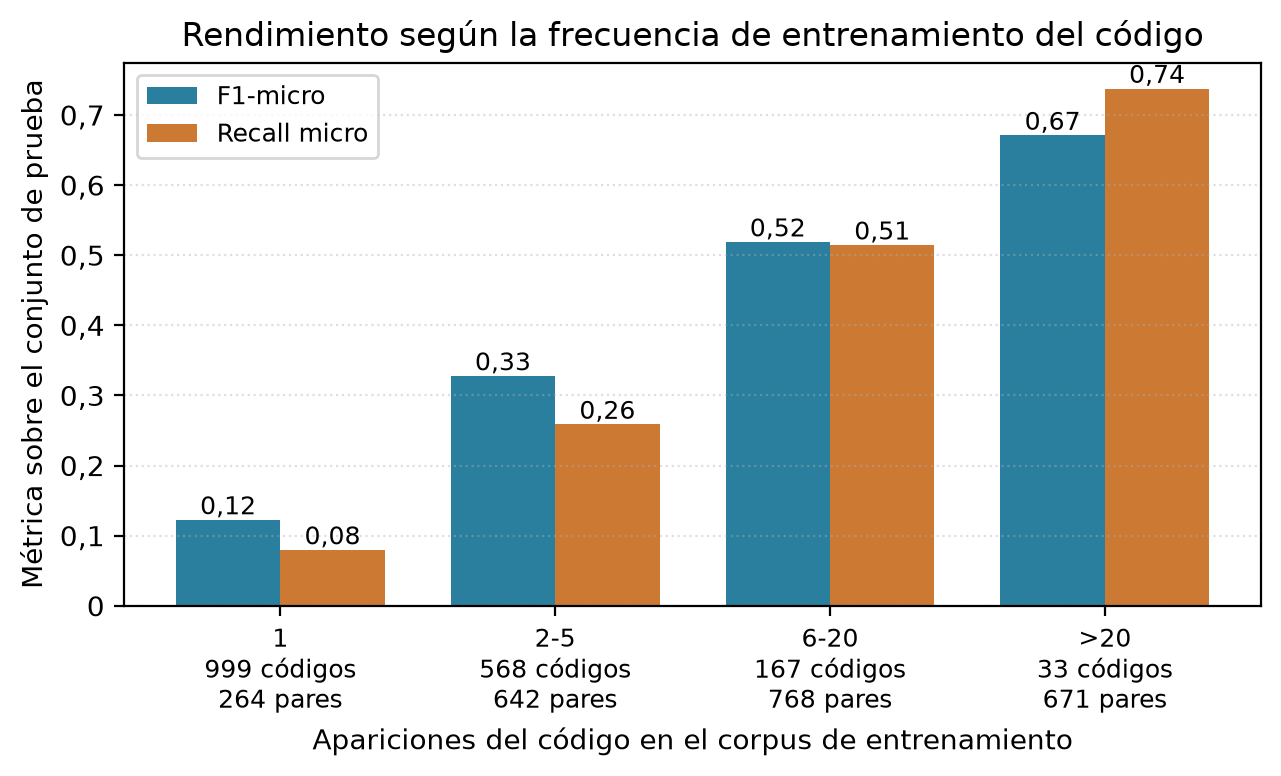
\includegraphics[width=0.75\textwidth]{figs/tfg_freq}
\caption{F1-micro y \emph{recall} sobre el conjunto de prueba según el número de apariciones del código en el corpus de entrenamiento (umbral 0,2, modelo desplegado). Bajo cada grupo se indica cuántos códigos lo forman y cuántos pares del \emph{gold} aportan.}
\label{fig:freq}
\end{figure}

La Figura~\ref{fig:benchmark} representa gráficamente esa clasificación y la Figura~\ref{fig:chapters} desglosa el rendimiento del modelo por capítulo CIE-10. La cifra reportada corresponde al modelo desplegado, que es el sistema que este trabajo presenta; la comparación de los candidatos que llevó a elegirlo está en la sección~\ref{sec:anexoH-candidatos}. Una observación preliminar recogida en el Anexo~\ref{cap:AnexoF} (sección~\ref{sec:anexoF-map}) apunta a que promediar las salidas de varias ejecuciones reduce la varianza y mejora el MAP; no se ha diseñado ni evaluado un sistema de combinación como tal, por lo que no se reporta como resultado y queda planteado como línea futura.

\begin{table}[h]
\centering
\small
\caption{Comparación con los sistemas del \emph{benchmark} CodiEsp-D (CLEF 2020)~\protect\cite{miranda2020}. Todas las métricas se calculan sobre el conjunto de prueba. Los equipos externos entregan listas de códigos ordenados por confianza (sin umbral de decisión), lo que explica sus valores de F1 muy bajos con \emph{recall} alto; el F1 de este trabajo corresponde a una decisión binaria con umbral global de 0,2, medida sobre el \emph{gold} alcanzable (sobre el completo, el \emph{recall} es 0,379 y el F1 0,444), y no es directamente comparable con esa columna. La métrica homogénea es el MAP por documento. Las dos filas sombreadas son este trabajo. Generada con \texttt{make ai-eval-test} (fila del clasificador solo, \texttt{model/\allowbreak{}eval\_test.json}) y \texttt{make ai-motores} (fila fusionada, \texttt{model/\allowbreak{}comparativa\_motores.json}); las filas de los demás equipos se transcriben de la Tabla~7 de~\cite{miranda2020}.}
\label{tab:codiesp-comparativa}
\begin{tabular}{P{3.6cm}P{4.0cm}rrrr}
\hline
\textbf{Sistema} & \textbf{Enfoque} & \textbf{P} & \textbf{R} & \textbf{F1} & \textbf{MAP} \\
\hline
IXA-AAA & XGBoost + BERT Multilingüe & 0{,}004 & 0{,}858 & 0{,}009 & \textbf{0{,}593} \\
\rowcolor{gray!15}
\textbf{Modo fusionado} & Clasificador + diccionario en un solo \emph{ranking} & 0{,}642 & 0{,}582 & 0{,}610 & \textbf{0{,}554}$^{*}$ \\
IAM & Diccionario + coincidencia exacta/Levenshtein & 0{,}817 & 0{,}592 & \textbf{0{,}687} & 0{,}521 \\
FLE & Sistema clínico multilingüe propietario & 0{,}740 & 0{,}633 & 0{,}679 & 0{,}519 \\
The Mental Strokers & BETO \emph{fine-tuning} & 0{,}759 & 0{,}638 & 0{,}591 & 0{,}517 \\
LSI-UNED & Recuperación de información + expansión & 0{,}253 & 0{,}688 & 0{,}370 & 0{,}517 \\
Anuj & BERT + búsqueda léxica & 0{,}741 & 0{,}621 & 0{,}676 & 0{,}505 \\
MEDIA & Ensamble con BETO & 0{,}735 & 0{,}630 & 0{,}629 & 0{,}488 \\
ICB-UMA~\cite{lopezgarcia2020icb} & BERT-SciELO \emph{fine-tuning} & 0{,}004 & 0{,}897 & 0{,}009 & 0{,}482 \\
\rowcolor{gray!15}
\textbf{Este trabajo (clasificador solo)} & RigoBERTa-Clinical \emph{fine-tuning} & 0{,}536 & 0{,}459 & 0{,}495 & 0{,}454 \\
IMS & CNN + atención & 0{,}373 & 0{,}709 & 0{,}474 & 0{,}449 \\
\hline
\end{tabular}

\vspace{2mm}
{\footnotesize Nota: en la fuente, las filas de The Mental Strokers (F1 0,591), MEDIA (0,629) e IMS (0,474) no cumplen $F1=2PR/(P+R)$ con las P y R impresas (daría 0,693, 0,678 y 0,489); se transcriben tal cual, y la discrepancia podría deberse a que cada columna procede de una ejecución distinta del equipo, pero el artículo no lo aclara.

\vspace{1mm}
\footnotesize $^{*}$ El modo fusionado combina el clasificador y el diccionario en un único
\emph{ranking} y está implementado en el motor (\texttt{engine=fused}), pero la configuración que
el sistema sirve por defecto es la del clasificador solo. Su cifra procede de
\texttt{make ai-motores} (\texttt{ai\_engine/\allowbreak{}motores\_eval.py}), que reproduce la fusión tal como
la implementa el motor y deja el barrido de $\beta$ en \texttt{model/\allowbreak{}fusion\_sweep.json}: medido en
esa misma pasada, el clasificador solo obtiene 0,454, la misma cifra que da la evaluación en
precisión completa, de modo que la ganancia atribuible a la fusión es de 10,0 puntos en ambas
procedencias. Se muestran las dos configuraciones porque ambas son ejecutables.}
\end{table}

\begin{figure}[ht]
\centering
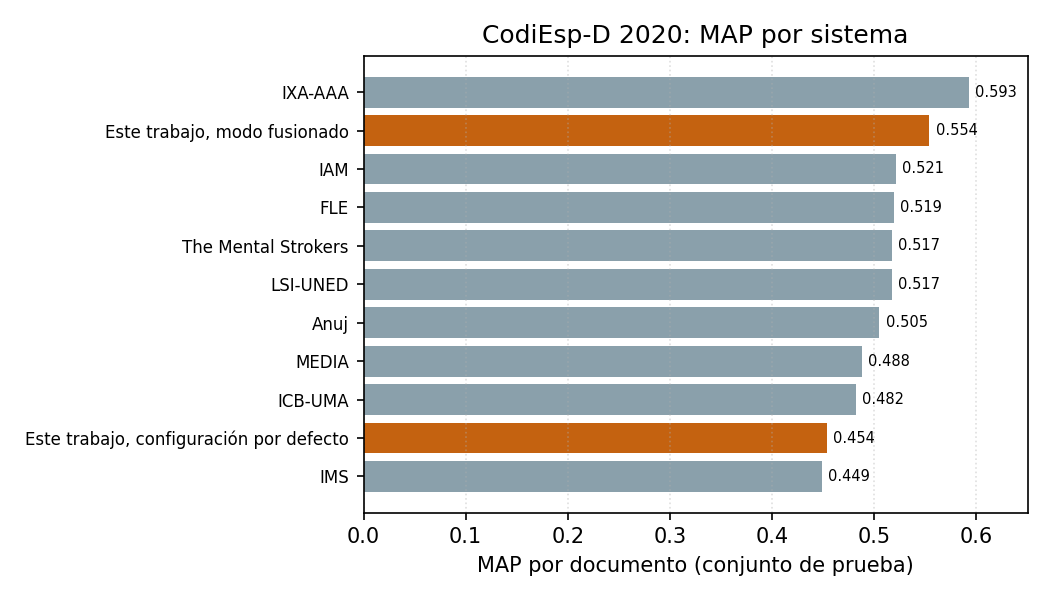
\includegraphics[width=0.8\textwidth]{figs/tfg_benchmark}
\caption[MAP por documento de los sistemas del \emph{benchmark} CodiEsp-D 2020 sobre el conjunto de prueba, con este trabajo resaltado]{MAP por documento de los sistemas del \emph{benchmark} CodiEsp-D 2020 sobre el conjunto de prueba, con este trabajo resaltado. Las primeras posiciones las ocupan \emph{ensembles} y diccionarios construidos manualmente.}
\label{fig:benchmark}
\end{figure}

\begin{figure}[ht]
\centering
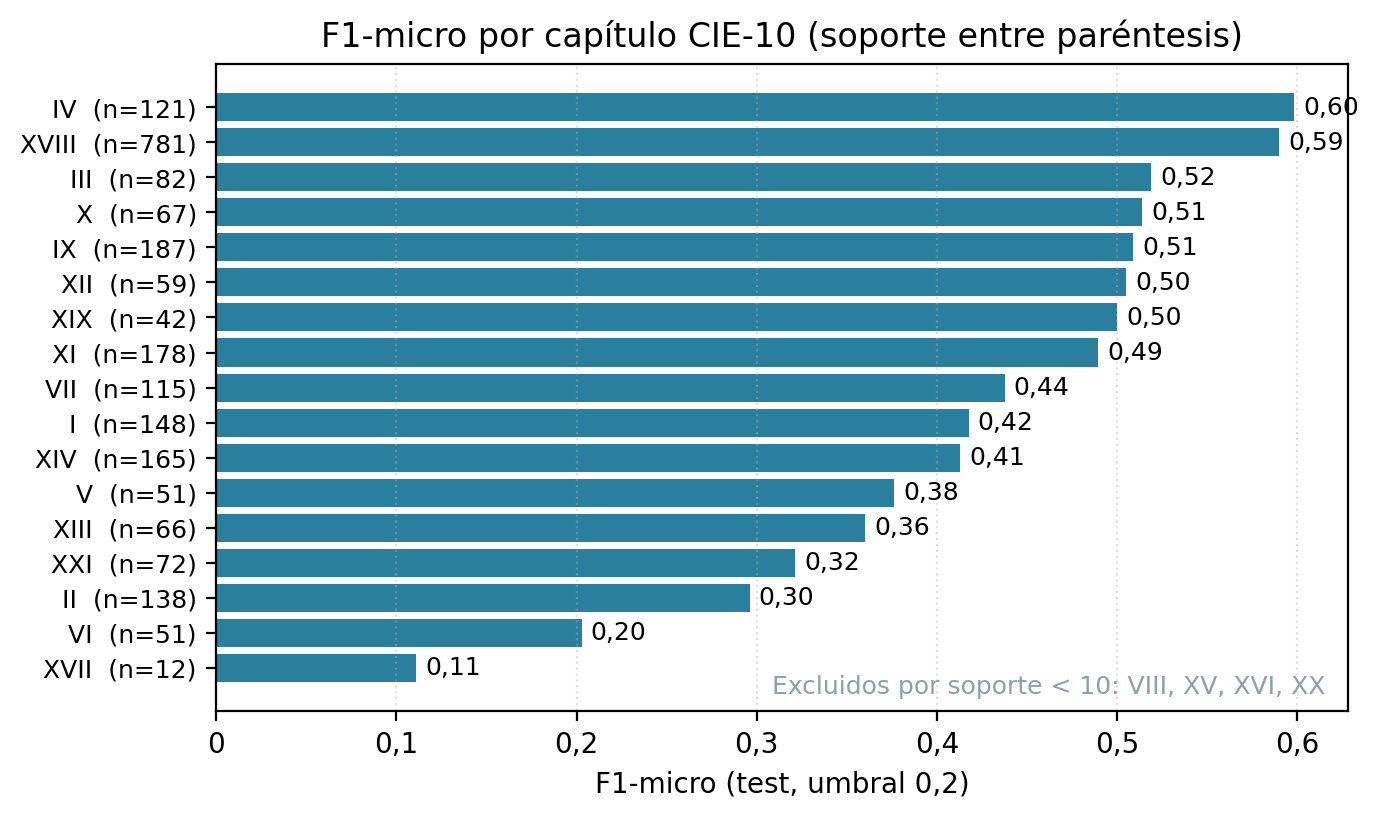
\includegraphics[width=0.75\textwidth]{figs/tfg_chapters}
\caption[F1-micro por capítulo CIE-10 sobre el conjunto de prueba (umbral 0,2, modelo desplegado), con el soporte de cada capítulo entre paréntesis]{F1-micro por capítulo CIE-10 sobre el conjunto de prueba (umbral 0,2, modelo desplegado), con el soporte de cada capítulo entre paréntesis. Se excluyen los capítulos con menos de diez pares en el \emph{gold} (VIII, XV, XVI y XX), donde el F1 carece de sentido estadístico. La equivalencia entre cada número romano y el capítulo de la CIE-10-ES se recoge en la Tabla~\ref{tab:capitulos-cie10} del Anexo~\ref{cap:AnexoG}.}
\label{fig:chapters}
\end{figure}

A nivel de capítulo la relación con la frecuencia de entrenamiento es solo moderada ($r=0{,}40$ sobre los diecisiete capítulos con soporte suficiente, una muestra pequeña, por lo que es una cifra orientativa), bastante más débil que la que se observa por código en la Figura~\ref{fig:freq}. Una razón probable es que un capítulo agrupa códigos muy heterogéneos, de modo que su F1 depende menos del volumen total de ejemplos que de cómo se reparten: dos capítulos con el mismo número de pares rinden de forma muy distinta según si esos pares se concentran en unos pocos códigos o se dispersan en muchos.

El capítulo~XVII (malformaciones congénitas) es el que peor rinde entre los capítulos con soporte suficiente, con F1-micro de 0,111 sobre 82 pares de entrenamiento. Con solo 12 pares en el \emph{gold} de prueba, esa cifra equivale a un acierto sobre pocas propuestas y es muy inestable; probablemente refleja códigos de malformaciones muy específicos y dispersos, con pocos ejemplos cada uno, más que una dificultad propia del capítulo. Como ilustración del mecanismo, y no como prueba, el capítulo~VI (enfermedades del sistema nervioso) permite aislarlo del volumen total: tiene exactamente el mismo soporte en prueba que el capítulo~V (51 pares) y una frecuencia de entrenamiento comparable (125 pares frente a 158), pero un F1 de 0,203 frente a 0,376, casi la mitad. La diferencia está en la concentración: los 125 pares del capítulo~VI se reparten entre \textbf{67 códigos distintos} (1,9 apariciones por código, y el más frecuente aparece solo ocho veces), mientras que los 158 del capítulo~V se concentran en \textbf{47 códigos} dominados por un puñado muy repetido, encabezado por los códigos de consumo de tabaco (\texttt{F17.210} aparece 28 veces) y la depresión no especificada (\texttt{F32.9}, 14 veces). Con un solo par de capítulos no se puede generalizar, pero el capítulo~VI se parece a la cola larga pura: neurología con muchos diagnósticos diferentes y casi ningún ejemplo por diagnóstico.

\subsubsection*{En qué se equivoca el modelo}

Las métricas agregadas dicen cuánto falla el clasificador, no en qué falla. Para saberlo se etiqueta cada error del conjunto de prueba según su distancia al código correcto: si comparte el bloque de tres caracteres con alguno de los anotados en ese documento, el error es de especificidad (el modelo entendió la patología y erró el grado de detalle); si comparte capítulo pero no bloque, erró dentro del área clínica correcta; si cae en otro capítulo, es un error de comprensión. El análisis se genera con \texttt{make ai-error-analysis} sobre el modelo desplegado (umbral 0,2) y queda en \texttt{model/error\_analysis.json}.

Lo primero que revela es que el modelo \textbf{subpredice}: propone 8,04 códigos por documento frente a los 11,37 anotados. No es un fallo de calibración menor, es la explicación directa de que el \emph{recall} quede por debajo de la precisión, y encaja con un umbral fijo aplicado a probabilidades que el desequilibrio de clases mantiene bajas.

\begin{table}[h]
\centering
\small
\caption{Errores del modelo sobre el conjunto de prueba, clasificados por distancia al código correcto (umbral 0,2, modelo desplegado). Generada con \texttt{make ai-error-analysis} (\texttt{model/\allowbreak{}error\_analysis.json}).}
\label{tab:analisis-error}
\begin{tabular}{lrrrr}
\hline
 & \textbf{Total} & \textbf{Mismo bloque} & \textbf{Mismo capítulo} & \textbf{Otro capítulo} \\
\hline
Falsos positivos & 933 & 209 (22,4\,\%) & 586 (62,8\,\%) & 138 (14,8\,\%) \\
Falsos negativos & 1.765 & 230 (13,0\,\%) & 847 (48,0\,\%) & 688 (39,0\,\%) \\
\hline
\end{tabular}
\end{table}

La lectura de la Tabla~\ref{tab:analisis-error} es favorable en un sentido y preocupante en otro. Cuando el modelo propone un código que no estaba anotado, el 85,2\,\% de las veces acierta al menos el capítulo, y algo más de una quinta parte de esos casos son códigos hermanos del correcto: fallos de grado de detalle, no de entendimiento. Un codificador que revise esa lista descarta el código pero conserva la pista. En cambio, el 39,0\,\% de los códigos que el modelo deja escapar pertenece a capítulos que no ha tocado en ese documento, de modo que el \emph{recall} no se arregla bajando el umbral: falta señal, no sensibilidad.

El desglose por código apunta a la misma causa en los dos sentidos. R52 («dolor, no especificado») encabeza los falsos positivos (39 casos) y aparece también entre los falsos negativos (20, empatado con R69, «enfermedad, no especificada»); completan el grupo N28.9 («trastorno del riñón y del uréter, no especificado», 22 falsos positivos) y R53.1 («astenia», 22). Son códigos residuales, los que el manual reserva para cuando el informe menciona el hallazgo pero no lo concreta. Asignarlos correctamente depende de lo que el documento \emph{no} dice, y un clasificador que puntúa cada etiqueta a partir de lo que sí aparece en el texto no tiene forma de representar esa ausencia. Es una limitación de la formulación del problema, no del entrenamiento, y por eso conviene declararla en lugar de atribuirla a falta de datos.

\paragraph{Nota sobre reproducibilidad y variabilidad entre ejecuciones.}
\begin{sloppypar}
El script de entrenamiento admite fijar la semilla aleatoria (\emph{random seed}) con \texttt{--seed}, pero no se utilizó en los experimentos. Esta decisión fue deliberada durante la fase exploratoria: fijar la semilla habría requerido activar \texttt{torch.use\_deterministic\_algorithms} y \texttt{CUBLAS\_WORKSPACE\_CONFIG}, lo que deshabilita kernels CUDA optimizados e incrementa el tiempo de entrenamiento de forma apreciable. En un proceso iterativo de decenas de ejecuciones (más de setenta registradas a fecha de cierre de este documento), ese sobrecoste habría sido prohibitivo.
\end{sloppypar}

La contrapartida es que los resultados no son exactamente reproducibles. Las fuentes de no-determinismo son tres: la inicialización aleatoria de la cabeza clasificadora, el orden de los mini-batches en cada época y las operaciones CUDA no deterministas (operaciones de reducción en paralelo, Flash Attention). En la práctica, la variabilidad observada entre ejecuciones con configuración idéntica es de $\pm 0{,}01$ en F1-micro, lo que no altera las conclusiones comparativas entre pasos pero sí impide replicar el valor exacto 0,4945 del paso~36. Los experimentos del 33 al 35 sirven para confirmar que esa configuración es robusta, no para superarla de forma reproducible.

Para un ciclo de reentrenamiento productivo con datos reales se recomienda fijar \texttt{--seed} y guardar la semilla en \texttt{config.json}, de modo que cada modelo desplegado sea auditable; el registro de ejecuciones ya dispone de una columna \texttt{seed} para anotarla.

\paragraph{Paso 36}
\begin{sloppypar}
Tras confirmar en los pasos 33--35 que ninguna modificación de hiperparámetros mejoraba de forma robusta la referencia 32b, se realizó una reejecución con la configuración exacta de 32b para explotar la variabilidad estocástica inherente al entrenamiento. El resultado fue F1-micro~\textbf{0,4945} en validación ($+0{,}006$ respecto a 32b) y F1-macro~0,119. La ejecución completó las 150~épocas en \textbf{27~minutos} ($\sim$11~s/época). La ganancia en F1-micro, dentro del intervalo de variabilidad estocástica $\pm 0{,}01$, se debe a una inicialización aleatoria más favorable. Sobre el conjunto de prueba el modelo obtiene F1-micro~0,4887 (umbral global 0,3) y un MAP por documento de \textbf{0,437} sobre el gold completo, la métrica oficial del \emph{benchmark}, lo que lo sitúa dentro del rango de los sistemas de CodiEsp 2020~\cite{miranda2020}, por detrás de los \emph{ensembles} y diccionarios de las primeras posiciones (véase Tabla~\ref{tab:codiesp-comparativa}). Este modelo, \texttt{classifier\_20260530T030233Z\_f1=0.4945.pt}, fue la ejecución de referencia durante la mayor parte del trabajo. La comparación final de candidatos sobre el conjunto de prueba (sección~\ref{sec:anexoH-candidatos}) lo desplazó en favor de la ejecución con pérdida de ordenación de la subsección~\ref{sec:anexoF-alineacion}, que lo supera en MAP, MAP fusionado y F1-micro a la vez; sus cifras se conservan aquí porque son las que sostienen la lectura de este paso.

El comando empleado para esta ejecución fue:
\begin{lstlisting}[language=bash,basicstyle=\small\ttfamily,showstringspaces=false]
FULL_CODES=1 MAX_LENGTH=512 FREEZE_LAYERS=20 LR=1e-4 DROPOUT=0.3 \
WEIGHT_DECAY=0.1 THRESHOLD=0.3 BATCH_SIZE=8 GRAD_ACCUM=4 \
EPOCHS=150 PATIENCE=20 LR_SCHEDULE=plateau LABEL_SMOOTHING=0.1 \
UNFREEZE_EVERY=30 UNFREEZE_LAYERS=4 UNFREEZE_LR_RATIO=0.1 \
LAMBDA_HIER=0.5 PRETRAIN_EPOCHS=10 \
PRETRAIN_TASKX="/data/codiesp_csvs/\
codiesp_X_source_train.csv \
 /data/codiesp_csvs/\
codiesp_X_source_validation.csv" \
make ai-train-gpu
\end{lstlisting}
\end{sloppypar}

\subsubsection{Aprendizaje continuo a partir de la retroalimentación de los usuarios}
\label{sec:continuous-learning}

Una limitación estructural del entrenamiento sobre CodiEsp es que los datos proceden de
un \emph{benchmark} con distribución fija. En un entorno clínico real, el modelo encontrará
patrones de redacción, abreviaturas y combinaciones de códigos que difieren del corpus de
entrenamiento. Para cerrar esta brecha, el sistema está diseñado para capturar señal de
retroalimentación de los propios codificadores y reutilizarla en ciclos de reentrenamiento
posteriores.

\paragraph{Datos capturados por el sistema.}
Cada sesión de análisis genera un registro inmutable de eventos en el \emph{event store}
del backend (véase la sección~\ref{sec:calidad}). Las proyecciones relacionales derivadas
de estos eventos contienen los elementos necesarios para construir muestras de
entrenamiento supervisado:

\begin{itemize}
 \item \textbf{Texto clínico} (\texttt{messages.content}): el informe enviado por el
 codificador clínico, que actúa como entrada $x$ del clasificador.
 \item \textbf{Validaciones} (\texttt{predicted\_codes.status = 'validated'}): códigos
 que el codificador ha confirmado como correctos. Constituyen etiquetas positivas
 $(y = 1)$ con respaldo humano.
 \item \textbf{Rechazos} (\texttt{predicted\_codes.status = 'rejected'}): códigos que el
 modelo predijo pero el codificador descartó. Señalan errores sistemáticos del modelo
 sobre textos reales de dominio.
 \item \textbf{Sugerencias manuales} (\texttt{code\_suggestions.suggested\_code}): códigos
 que el codificador añade manualmente cuando no aparecen entre las predicciones del
 modelo. Son la señal más valiosa del ciclo: representan \emph{falsos negativos} que el
 modelo no habría detectado de otro modo.
\end{itemize}

\paragraph{Limitación: sesgo de confirmación.}
El mecanismo de retroalimentación presenta una asimetría inherente. El codificador solo
valida o rechaza los códigos que el modelo ya ha sugerido; los códigos correctos que no
aparecen en el top-$k$ de predicciones permanecen invisibles salvo que el codificador los
añada explícitamente mediante la función de sugerencia manual. Esto implica que la
retroalimentación de validación/rechazo refuerza las predicciones existentes, pero no corrige los
falsos negativos estructurales del modelo. Por este motivo, las sugerencias manuales tienen
mayor peso informativo que las validaciones: cada sugerencia manual identifica un caso que
el modelo no cubrió.

\paragraph{Transformación al formato de entrenamiento.}
Para incorporar la retroalimentación al ciclo de entrenamiento, los datos de las proyecciones se
transforman al mismo formato CSV que CodiEsp: una fila por informe con el texto clínico
como campo \texttt{text} y la lista de códigos confirmados (validaciones más sugerencias
manuales) como campo \texttt{labels}, separados por punto y coma. El conjunto resultante
se combina con el corpus CodiEsp original antes de lanzar el entrenamiento:

\begin{equation*}
 \mathcal{D}_{\text{combinado}} = \mathcal{D}_{\text{CodiEsp}} \cup \mathcal{D}_{\text{retro}}
\end{equation*}

\paragraph{Estrategia de incorporación recomendada.}
En lugar de entrenar desde cero con el conjunto combinado, se recomienda partir del
\emph{checkpoint} del modelo en producción y realizar un \emph{fine-tuning} de pocas
épocas (5--10) sobre $\mathcal{D}_{\text{combinado}}$. Este enfoque tiene tres ventajas:
hereda el conocimiento adquirido durante el entrenamiento completo sobre CodiEsp, reduce
el tiempo de cómputo, y minimiza el riesgo de \emph{catastrophic forgetting} mediante una
tasa de aprendizaje reducida ($\eta \approx 2 \times 10^{-5}$). Antes de sustituir el
modelo en producción, el nuevo \emph{checkpoint} debe evaluarse sobre la partición de
validación de CodiEsp; si el F1-micro decrece más de un punto porcentual respecto al
modelo en producción, ese reentrenamiento se descarta.

\paragraph{Requisito de volumen mínimo.}
Con menos de 100 muestras nuevas, la relación señal/ruido de la retroalimentación no compensa
el coste del reentrenamiento. El ciclo de mejora continua se activa cuando se acumulan
al menos 100--200 informes con al menos un código validado o sugerido manualmente.
Este umbral pretende que el conjunto de retroalimentación tenga diversidad suficiente para
generalizar y no sobreajustar a patrones específicos de un único codificador o servicio
hospitalario.

\subsection{Diseño del backend}
\label{sec:diseno-backend}

El backend es el orquestador central del sistema. Desarrollado en Elixir 1.19 con el \emph{framework} Phoenix 1.8, asume tres responsabilidades: gestionar la autenticación y el ciclo de vida de los usuarios, coordinar el flujo de análisis clínico entre el frontend y el motor de IA, y dar trazabilidad a las acciones sobre cada caso.

Para cumplir el requisito de trazabilidad clínica, el backend se organiza en torno al patrón CQRS y \emph{Event Sourcing} (sección~\ref{sec:calidad}), implementado mediante la biblioteca Commanded. Lo que aporta aquí es que cualquier acción, desde la creación de un análisis hasta la validación de un código individual, queda registrada con su marca temporal y su autoría (Figura~\ref{fig:admin-conversations}). Los comandos principales son: \texttt{RegisterUser}, \texttt{AnalyzeReport}, \texttt{ReceiveAIPrediction}, \texttt{ValidateCode} y \texttt{RejectCode}. Cada comando genera uno o más eventos que son procesados por proyectores que actualizan las vistas de lectura en PostgreSQL; la Figura~\ref{fig:cqrs-flujo} resume ese recorrido, desde el comando hasta los modelos de lectura. El esquema completo de eventos, comandos y tablas de proyección se documenta en el Anexo~\ref{cap:AnexoD}.

\begin{figure}[ht]
\centering
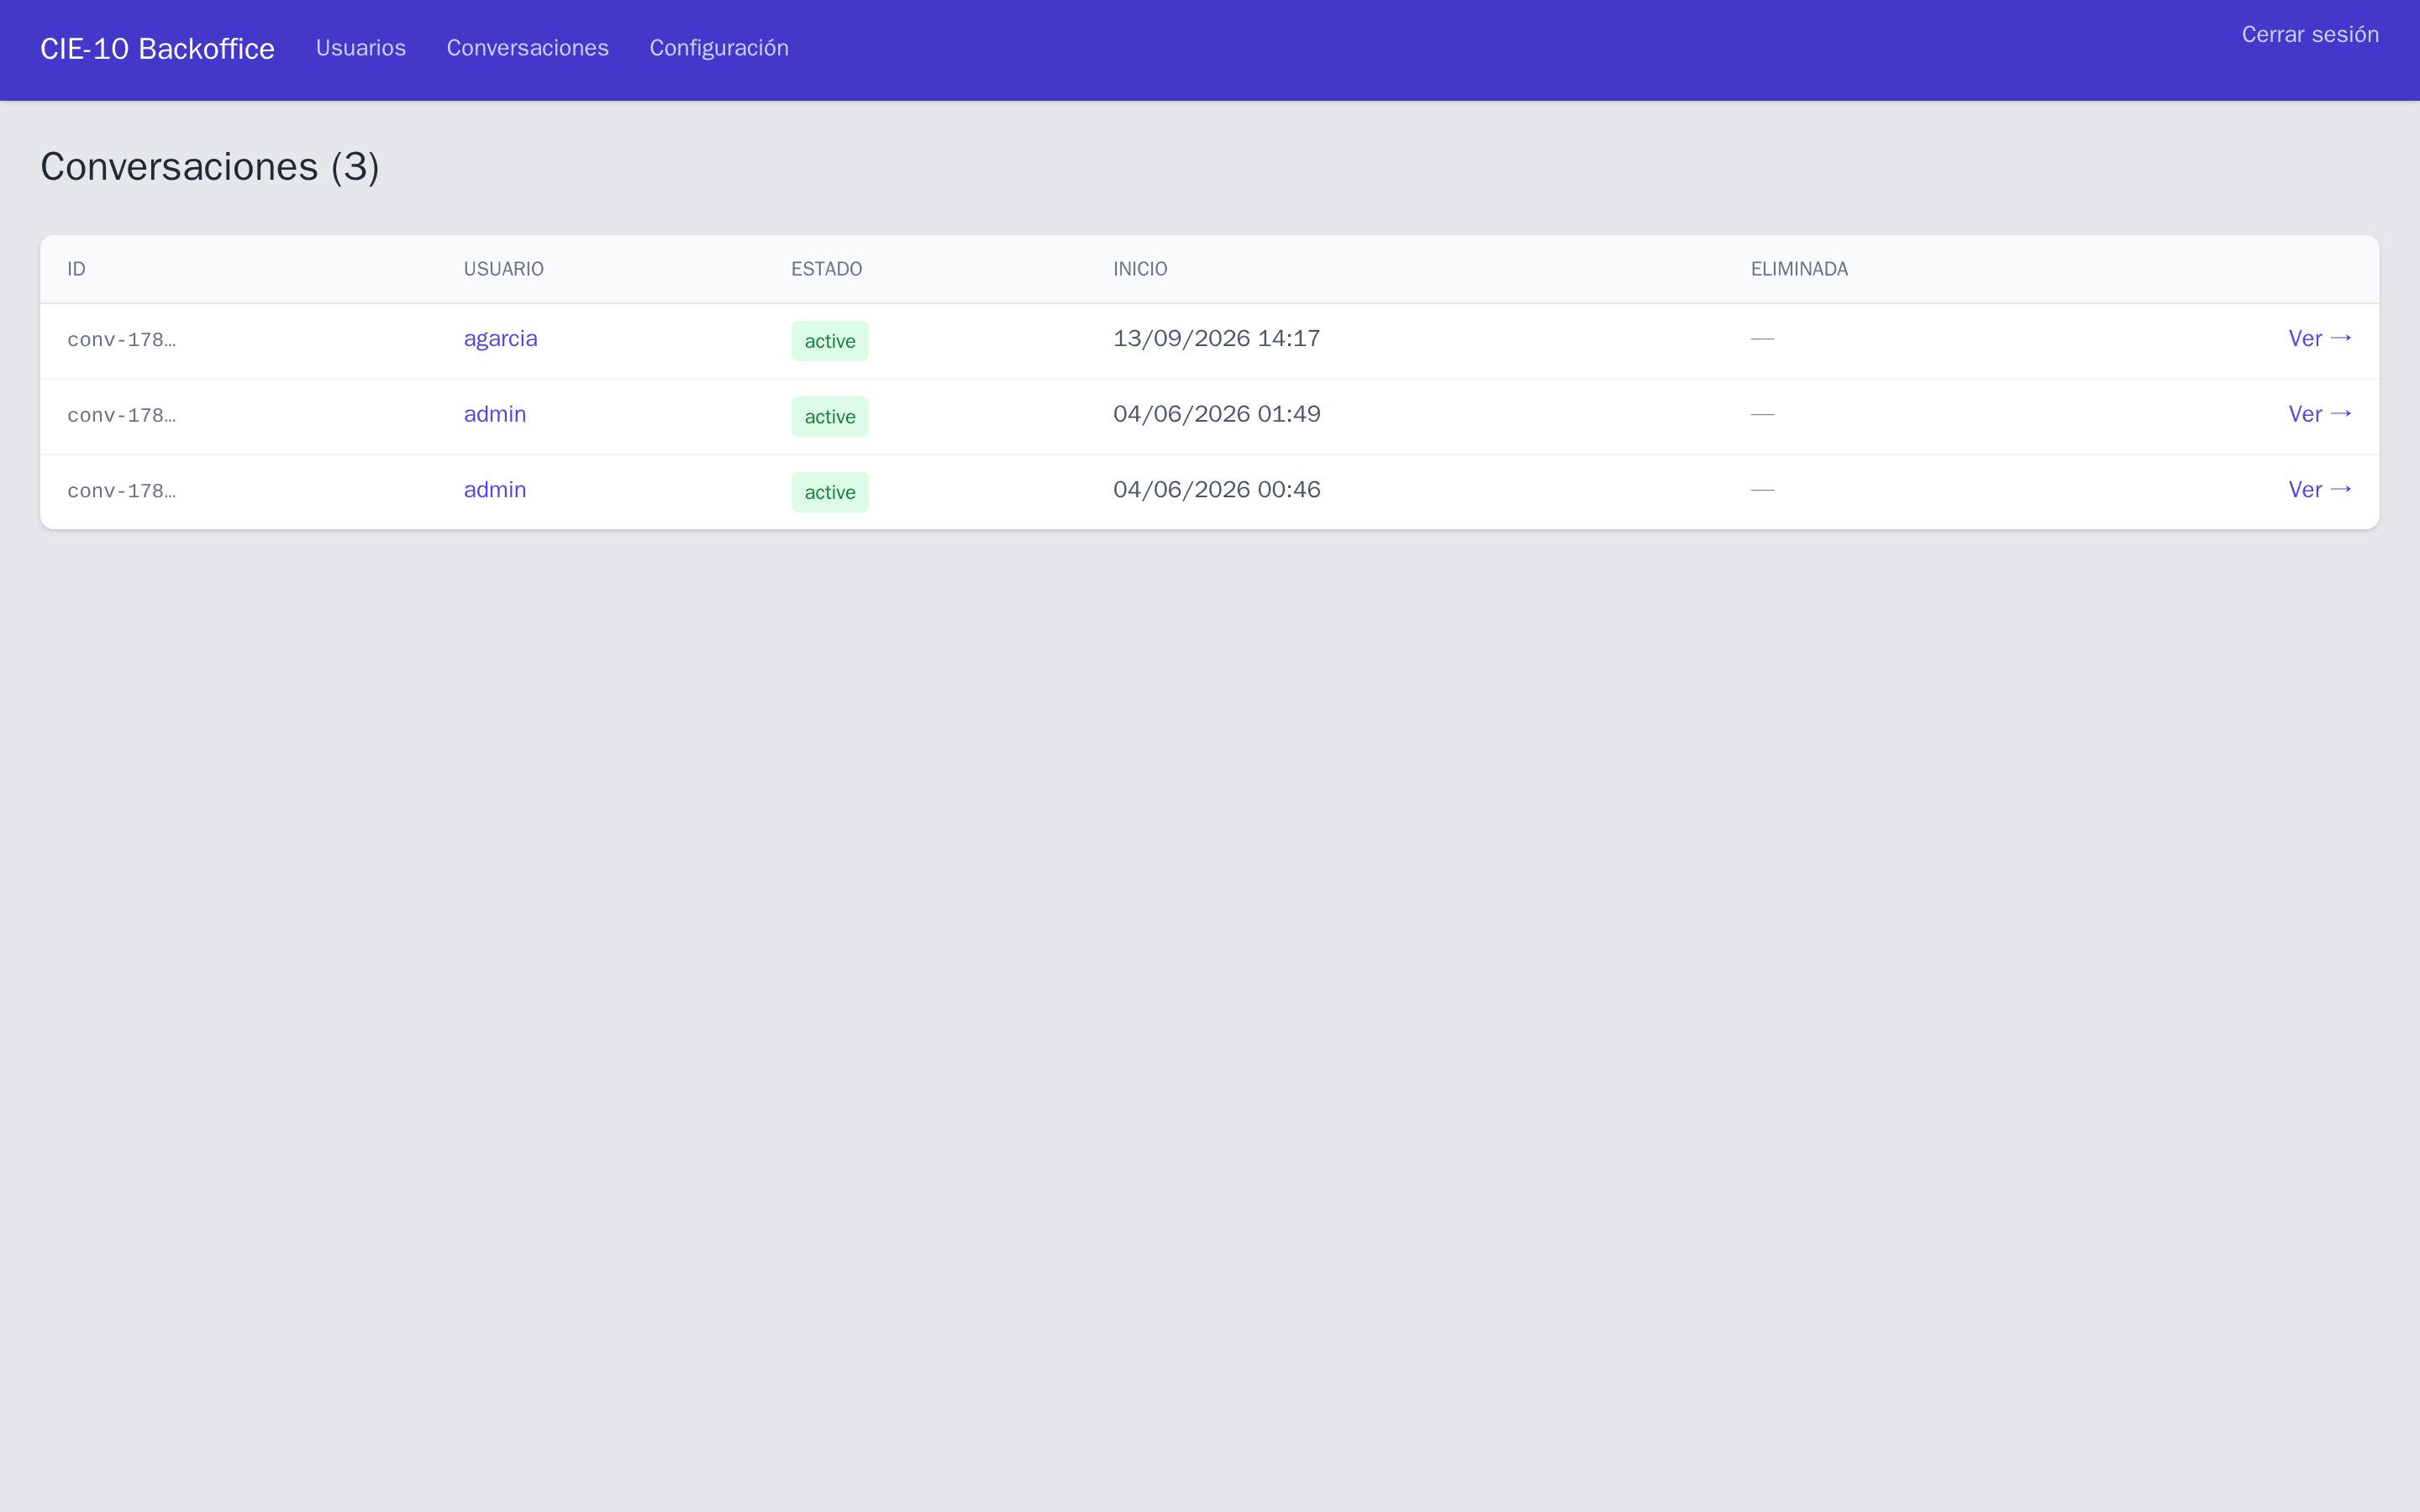
\includegraphics[width=0.9\textwidth, trim=0 1150 1180 0, clip]{figs/ui-admin-conversations}
\caption{Vista de administración de las conversaciones: cada análisis queda registrado con su usuario, estado y marca temporal, reflejo de la trazabilidad que aporta el \emph{Event Sourcing}.}
\label{fig:admin-conversations}
\end{figure}

\begin{figure}[ht]
\centering
\resizebox{\textwidth}{!}{% Diagrama de flujo CQRS / Event Sourcing
% Uso: % Diagrama de flujo CQRS / Event Sourcing
% Uso: % Diagrama de flujo CQRS / Event Sourcing
% Uso: \input{figs/cqrs-flujo} dentro de figure+\centering+\resizebox{\textwidth}{!}{...}
%
% Flujo: Comando → Manejador → Agregado → Evento → EventStore → Proyector → Modelo de lectura

\begin{tikzpicture}[
  every node/.style={font=\small\sffamily},
  %--- Escritura (lado izquierdo) ---
  cmd/.style={
    draw=palered!80, fill=palered!10, thick,
    rectangle, rounded corners=4pt,
    minimum width=2.6cm, minimum height=1.1cm,
    align=center
  },
  handler/.style={
    draw=gray!60, fill=gray!10, thick,
    rectangle, rounded corners=4pt,
    minimum width=2.6cm, minimum height=1.1cm,
    align=center
  },
  agg/.style={
    draw=aquaESI!80, fill=aquaESI!15, thick,
    rectangle, rounded corners=4pt,
    minimum width=2.6cm, minimum height=1.1cm,
    align=center
  },
  evt/.style={
    draw=ocre!80, fill=ocre!15, thick,
    rectangle, rounded corners=4pt,
    minimum width=2.6cm, minimum height=1.1cm,
    align=center
  },
  store/.style={
    draw=turquesa!80, fill=turquesa!15, thick,
    cylinder, shape border rotate=90,
    minimum height=1.4cm, minimum width=2.4cm,
    align=center
  },
  proj/.style={
    draw=gray!70, fill=gray!12, thick,
    rectangle, rounded corners=4pt,
    minimum width=2.6cm, minimum height=1.1cm,
    align=center
  },
  read/.style={
    draw=aquaESI!60, fill=aquaESI!10, thick,
    rectangle, rounded corners=4pt,
    minimum width=2.6cm, minimum height=1.1cm,
    align=center
  },
  %--- Flechas ---
  arr/.style={->, >=Stealth, thick},
  lbl/.style={font=\small\sffamily, midway, fill=white,
              inner sep=1.5pt, draw=gray!25, rounded corners=2pt},
  node distance=0.5cm and 0.9cm
]

%--- LADO ESCRITURA (fila superior) ---
\node[cmd] (cmd1) at (0,0) {
  \textbf{Comando}\\
  \footnotesize AnalyzeReport,\\ValidateCode
};

\node[agg, right=2.2cm of cmd1] (agg) {
  \textbf{Agregado}\\
  \footnotesize Analysis\\(estado)
};

\node[evt, right=2.0cm of agg] (evt1) {
  \textbf{Evento}\\
  \footnotesize ReportAnalyzed,\\CodeValidated
};

\node[store, right=2.2cm of evt1] (es) {
  \textbf{Event Store}\\
  \footnotesize PostgreSQL
};

%--- PROYECTOR (fila inferior) ---
\node[proj, below=1.4cm of es] (proj) {
  \textbf{Proyector}\\
  \footnotesize una proyección\\por evento
};

\node[read, left=1.2cm of proj, minimum width=5.4cm, text width=5.2cm] (r1) {
  \textbf{Modelo de lectura}\\
  \footnotesize conversations, analysis\_cards,\\predicted\_codes
};

%--- FLECHAS DE ESCRITURA ---
\draw[arr] (cmd1) -- node[lbl, above]{ejecuta} (agg);
\draw[arr] (agg)  -- node[lbl, above]{emite} (evt1);
\draw[arr] (evt1) -- node[lbl, above]{guarda} (es);

%--- FLECHA EventStore → Proyector ---
\draw[arr] (es) -- node[lbl, right]{se suscribe} (proj);

\draw[arr] (proj) -- node[lbl, above]{actualiza} (r1);

%--- ETIQUETAS DE ZONA ---
\node[font=\small\sffamily\bfseries, palered!80]
  at ($(cmd1)!0.5!(evt1) + (0,1.5)$) {Lado escritura (comandos)};

\node[font=\small\sffamily\bfseries, aquaESI!80]
  at ($(r1)!0.5!(proj) + (0,-1.5)$) {Lado lectura (consultas y proyecciones)};

%--- SEPARADOR ---
\draw[dashed, gray!50, thick]
  ($(es.south)!0.5!(proj.north)$) ++(-10,0) -- ++(13,0);

\end{tikzpicture}
 dentro de figure+\centering+\resizebox{\textwidth}{!}{...}
%
% Flujo: Comando → Manejador → Agregado → Evento → EventStore → Proyector → Modelo de lectura

\begin{tikzpicture}[
  every node/.style={font=\small\sffamily},
  %--- Escritura (lado izquierdo) ---
  cmd/.style={
    draw=palered!80, fill=palered!10, thick,
    rectangle, rounded corners=4pt,
    minimum width=2.6cm, minimum height=1.1cm,
    align=center
  },
  handler/.style={
    draw=gray!60, fill=gray!10, thick,
    rectangle, rounded corners=4pt,
    minimum width=2.6cm, minimum height=1.1cm,
    align=center
  },
  agg/.style={
    draw=aquaESI!80, fill=aquaESI!15, thick,
    rectangle, rounded corners=4pt,
    minimum width=2.6cm, minimum height=1.1cm,
    align=center
  },
  evt/.style={
    draw=ocre!80, fill=ocre!15, thick,
    rectangle, rounded corners=4pt,
    minimum width=2.6cm, minimum height=1.1cm,
    align=center
  },
  store/.style={
    draw=turquesa!80, fill=turquesa!15, thick,
    cylinder, shape border rotate=90,
    minimum height=1.4cm, minimum width=2.4cm,
    align=center
  },
  proj/.style={
    draw=gray!70, fill=gray!12, thick,
    rectangle, rounded corners=4pt,
    minimum width=2.6cm, minimum height=1.1cm,
    align=center
  },
  read/.style={
    draw=aquaESI!60, fill=aquaESI!10, thick,
    rectangle, rounded corners=4pt,
    minimum width=2.6cm, minimum height=1.1cm,
    align=center
  },
  %--- Flechas ---
  arr/.style={->, >=Stealth, thick},
  lbl/.style={font=\small\sffamily, midway, fill=white,
              inner sep=1.5pt, draw=gray!25, rounded corners=2pt},
  node distance=0.5cm and 0.9cm
]

%--- LADO ESCRITURA (fila superior) ---
\node[cmd] (cmd1) at (0,0) {
  \textbf{Comando}\\
  \footnotesize AnalyzeReport,\\ValidateCode
};

\node[agg, right=2.2cm of cmd1] (agg) {
  \textbf{Agregado}\\
  \footnotesize Analysis\\(estado)
};

\node[evt, right=2.0cm of agg] (evt1) {
  \textbf{Evento}\\
  \footnotesize ReportAnalyzed,\\CodeValidated
};

\node[store, right=2.2cm of evt1] (es) {
  \textbf{Event Store}\\
  \footnotesize PostgreSQL
};

%--- PROYECTOR (fila inferior) ---
\node[proj, below=1.4cm of es] (proj) {
  \textbf{Proyector}\\
  \footnotesize una proyección\\por evento
};

\node[read, left=1.2cm of proj, minimum width=5.4cm, text width=5.2cm] (r1) {
  \textbf{Modelo de lectura}\\
  \footnotesize conversations, analysis\_cards,\\predicted\_codes
};

%--- FLECHAS DE ESCRITURA ---
\draw[arr] (cmd1) -- node[lbl, above]{ejecuta} (agg);
\draw[arr] (agg)  -- node[lbl, above]{emite} (evt1);
\draw[arr] (evt1) -- node[lbl, above]{guarda} (es);

%--- FLECHA EventStore → Proyector ---
\draw[arr] (es) -- node[lbl, right]{se suscribe} (proj);

\draw[arr] (proj) -- node[lbl, above]{actualiza} (r1);

%--- ETIQUETAS DE ZONA ---
\node[font=\small\sffamily\bfseries, palered!80]
  at ($(cmd1)!0.5!(evt1) + (0,1.5)$) {Lado escritura (comandos)};

\node[font=\small\sffamily\bfseries, aquaESI!80]
  at ($(r1)!0.5!(proj) + (0,-1.5)$) {Lado lectura (consultas y proyecciones)};

%--- SEPARADOR ---
\draw[dashed, gray!50, thick]
  ($(es.south)!0.5!(proj.north)$) ++(-10,0) -- ++(13,0);

\end{tikzpicture}
 dentro de figure+\centering+\resizebox{\textwidth}{!}{...}
%
% Flujo: Comando → Manejador → Agregado → Evento → EventStore → Proyector → Modelo de lectura

\begin{tikzpicture}[
  every node/.style={font=\small\sffamily},
  %--- Escritura (lado izquierdo) ---
  cmd/.style={
    draw=palered!80, fill=palered!10, thick,
    rectangle, rounded corners=4pt,
    minimum width=2.6cm, minimum height=1.1cm,
    align=center
  },
  handler/.style={
    draw=gray!60, fill=gray!10, thick,
    rectangle, rounded corners=4pt,
    minimum width=2.6cm, minimum height=1.1cm,
    align=center
  },
  agg/.style={
    draw=aquaESI!80, fill=aquaESI!15, thick,
    rectangle, rounded corners=4pt,
    minimum width=2.6cm, minimum height=1.1cm,
    align=center
  },
  evt/.style={
    draw=ocre!80, fill=ocre!15, thick,
    rectangle, rounded corners=4pt,
    minimum width=2.6cm, minimum height=1.1cm,
    align=center
  },
  store/.style={
    draw=turquesa!80, fill=turquesa!15, thick,
    cylinder, shape border rotate=90,
    minimum height=1.4cm, minimum width=2.4cm,
    align=center
  },
  proj/.style={
    draw=gray!70, fill=gray!12, thick,
    rectangle, rounded corners=4pt,
    minimum width=2.6cm, minimum height=1.1cm,
    align=center
  },
  read/.style={
    draw=aquaESI!60, fill=aquaESI!10, thick,
    rectangle, rounded corners=4pt,
    minimum width=2.6cm, minimum height=1.1cm,
    align=center
  },
  %--- Flechas ---
  arr/.style={->, >=Stealth, thick},
  lbl/.style={font=\small\sffamily, midway, fill=white,
              inner sep=1.5pt, draw=gray!25, rounded corners=2pt},
  node distance=0.5cm and 0.9cm
]

%--- LADO ESCRITURA (fila superior) ---
\node[cmd] (cmd1) at (0,0) {
  \textbf{Comando}\\
  \footnotesize AnalyzeReport,\\ValidateCode
};

\node[agg, right=2.2cm of cmd1] (agg) {
  \textbf{Agregado}\\
  \footnotesize Analysis\\(estado)
};

\node[evt, right=2.0cm of agg] (evt1) {
  \textbf{Evento}\\
  \footnotesize ReportAnalyzed,\\CodeValidated
};

\node[store, right=2.2cm of evt1] (es) {
  \textbf{Event Store}\\
  \footnotesize PostgreSQL
};

%--- PROYECTOR (fila inferior) ---
\node[proj, below=1.4cm of es] (proj) {
  \textbf{Proyector}\\
  \footnotesize una proyección\\por evento
};

\node[read, left=1.2cm of proj, minimum width=5.4cm, text width=5.2cm] (r1) {
  \textbf{Modelo de lectura}\\
  \footnotesize conversations, analysis\_cards,\\predicted\_codes
};

%--- FLECHAS DE ESCRITURA ---
\draw[arr] (cmd1) -- node[lbl, above]{ejecuta} (agg);
\draw[arr] (agg)  -- node[lbl, above]{emite} (evt1);
\draw[arr] (evt1) -- node[lbl, above]{guarda} (es);

%--- FLECHA EventStore → Proyector ---
\draw[arr] (es) -- node[lbl, right]{se suscribe} (proj);

\draw[arr] (proj) -- node[lbl, above]{actualiza} (r1);

%--- ETIQUETAS DE ZONA ---
\node[font=\small\sffamily\bfseries, palered!80]
  at ($(cmd1)!0.5!(evt1) + (0,1.5)$) {Lado escritura (comandos)};

\node[font=\small\sffamily\bfseries, aquaESI!80]
  at ($(r1)!0.5!(proj) + (0,-1.5)$) {Lado lectura (consultas y proyecciones)};

%--- SEPARADOR ---
\draw[dashed, gray!50, thick]
  ($(es.south)!0.5!(proj.north)$) ++(-10,0) -- ++(13,0);

\end{tikzpicture}
}
\caption{Flujo CQRS/\emph{Event Sourcing} del backend: desde el comando hasta los modelos de lectura.}
\label{fig:cqrs-flujo}
\end{figure}

El almacenamiento de eventos se implementa sobre PostgreSQL, sin recurrir a una base de datos dedicada para \emph{Event Sourcing} como EventStoreDB o Apache Kafka. Esta decisión (ADR-04, Anexo~\ref{cap:AnexoE}) reduce la complejidad operativa: un único sistema de base de datos para administrar, con soporte nativo y maduro en Commanded. Si el volumen de eventos creciera hasta niveles que saturaran PostgreSQL, lo que en el contexto clínico de un hospital de tamaño medio no se prevé a corto plazo, la migración a un \emph{broker} de mensajes como Kafka es viable sin cambios estructurales en el dominio, gracias a la inversión de dependencias que aísla los agregados y proyectores del adaptador de persistencia concreto (principio DIP, detallado en la sección~\ref{sec:calidad}).

La comunicación en tiempo real entre frontend y backend se realiza mediante canales WebSocket de Phoenix, tecnología que encaja de forma natural con el modelo de actores de la BEAM. El canal \texttt{ConversationChannel} gestiona el envío de informes, la recepción asíncrona de predicciones del motor de IA y la difusión de tarjetas de análisis al cliente a medida que se generan, sin necesidad de sondeo periódico. La especificación completa de los mensajes WebSocket y de la API REST se recoge en el Anexo~\ref{cap:AnexoC}.

\subsection{Diseño del frontend}

El frontend está desarrollado en Next.js 16 con React 19 y TypeScript. La interfaz utiliza Tailwind CSS 4 y la biblioteca de componentes shadcn/ui. La arquitectura de estado se basa en contextos de React: \texttt{AuthContext} gestiona la sesión del usuario, \texttt{ConversationContext} gestiona el estado del análisis activo y el historial, e \texttt{I18nContext} gestiona las traducciones de la interfaz (cinco idiomas, sección~\ref{sec:i18n}).

La configuración de URLs de backend y WebSocket se centraliza en \texttt{src/lib/config.ts}, que lee las variables de entorno \texttt{NEXT\_PUBLIC\_API\_URL} y \texttt{NEXT\_PUBLIC\_WS\_URL}, evitando cualquier dirección codificada directamente en el código.

El punto de entrada a la aplicación es la pantalla de inicio de sesión (Figura~\ref{fig:ui-login}), desde la que el usuario accede al panel de análisis descrito en la sección~\ref{sec:modelo-interfaz}.

\begin{figure}[ht]
\centering

\includegraphics[width=0.45\textwidth, trim=920 270 920 270, clip]{figs/ui-login}
\caption{Pantalla de inicio de sesión de la interfaz web.}
\label{fig:ui-login}
\end{figure}

\section{Implementación del sistema}

\subsection{Estructura del repositorio}

El repositorio se organiza en los siguientes directorios de alto nivel:

\begin{itemize}
 \item \texttt{ai\_engine/}: servicio FastAPI de inferencia. Contiene el módulo \texttt{classifier.py} con la clase \texttt{CIE10Classifier}, el script de entrenamiento \texttt{train.py}, el punto de entrada \texttt{main.py} y los artefactos del modelo entrenado en \texttt{model/}.
 \item \texttt{ai\_engine\_mock/}: versión simulada del motor de IA para desarrollo local, que devuelve predicciones ficticias sin necesidad de cargar el modelo BERT.
 \item \texttt{backend/}: aplicación Phoenix. La lógica de negocio se organiza en \texttt{lib/app/} (contextos, agregados, proyectores) y la capa web en \texttt{lib/app\_web/} (controladores, canales, \emph{plugs}).
 \item \texttt{frontend/}: aplicación Next.js. Los componentes de UI están en \texttt{src/components/}, los contextos en \texttt{src/contexts/} y la lógica de comunicación en \texttt{src/lib/}.
 \item \texttt{training/}: entorno de entrenamiento separado del servicio de producción. Contiene los scripts de descarga de datos en \texttt{csv\_import\_scripts/}, los notebooks de análisis estadístico en \texttt{data\_analysis/} y los notebooks de entrenamiento en \texttt{bert-classifier/}.
\end{itemize}

El repositorio se gestiona con Git. El historial de commits refleja el desarrollo incremental del sistema y puede consultarse en el repositorio del proyecto.

\subsection{Pipeline de entrenamiento}

El entrenamiento del modelo se orquesta mediante el \texttt{Makefile} de la raíz del proyecto. El entrenamiento con GPU se lanza con \texttt{make ai-train-gpu} (con CPU, \texttt{make ai-train}) y deja los artefactos del modelo en el directorio \texttt{ai\_engine/model/}.

El script \texttt{train.py} acepta los siguientes parámetros configurables por línea de comandos: ruta a los ficheros de entrenamiento y validación, ruta al fichero de descripciones CIE-10-ES, directorio de salida, nombre del modelo base, longitud máxima de secuencia, número de épocas, tamaño de batch, acumulación de gradientes y dispositivo de cómputo. El modelo guarda un \emph{checkpoint} del mejor resultado en validación (por F1-micro), el mapeo código-índice y un fichero \texttt{config.json} con todos los hiperparámetros, de modo que la inferencia posterior no requiere conocer los parámetros de entrenamiento.

\subsection{Servicio de inferencia}

El servicio de inferencia (\texttt{ai\_engine/main.py}) es una aplicación FastAPI que carga el modelo BERT al arrancar mediante el mecanismo de ciclo de vida (\texttt{lifespan}). Expone los siguientes endpoints:

\begin{itemize}
 \item \texttt{POST /predict}: recibe el texto del informe y devuelve los códigos CIE-10 predichos. El resumen médico se genera por separado.
 \item \texttt{POST /summarize/stream}: genera el resumen o paráfrasis del informe en tiempo real, devolviendo los tokens del LLM de forma incremental mediante NDJSON (\emph{newline-delimited JSON}).
 \item \texttt{GET /}: comprueba que el servicio está en funcionamiento y que el modelo está cargado.
\end{itemize}

Si el directorio del modelo no existe al arrancar, el servicio se inicia igualmente y devuelve un error 503 en las peticiones de predicción, lo que facilita el desarrollo sin necesidad de tener el modelo entrenado.

\subsubsection{Módulo de generación de resúmenes}
\label{sec:resumidor}

Además de los códigos CIE-10, el sistema genera para cada informe un \textbf{resumen clínico} que acompaña a la propuesta de codificación y ayuda al codificador a situar rápidamente el caso. La generación se delega en un modelo de lenguaje generativo (LLM) ligero, independiente del clasificador, expuesto en el \emph{endpoint} \texttt{POST /summarize/stream}.

El modelo se ejecuta con \texttt{llama-cpp-python} sobre pesos cuantizados en formato GGUF (cuantización Q4\_K\_M), lo que permite servir el resumen \textbf{en CPU} sin GPU dedicada, en coherencia con la arquitectura de despliegue de bajo coste (Anexo~\ref{cap:AnexoI}). El modelo base es configurable, se evaluaron Gemma~3~4B, Gemma~E4B y E2B, Phi-4-mini y Qwen2.5-3B, con una ventana de contexto de 8.192 \emph{tokens}, suficiente para los informes del corpus. El componente admite dos modos: \texttt{summary}, que produce un resumen conciso (máximo 80 palabras), y \texttt{paraphrase}, que reformula el informe conservando todos los datos clínicos. El modelo activo, el modo y los \emph{prompts} de sistema y de usuario se ajustan en tiempo de ejecución desde el \emph{backoffice} de administración, sin necesidad de redesplegar (véase la sección~\ref{sec:feature-toggle}).

La generación emplea una temperatura baja (0,2) para favorecer salidas deterministas y fieles al texto original, y se emite token a token mediante \emph{streaming}, como se detalla en la sección~\ref{sec:streaming-resumen}. Al tratarse de una funcionalidad de apoyo (no forma parte del núcleo de codificación), el resumidor está desactivado por defecto en el despliegue de producción (\texttt{SUMMARIZER\_MODEL=none}) y se habilita bajo demanda, de modo que el coste computacional del LLM solo se asume cuando se desea esta ayuda.

\paragraph{Modelos evaluados.} El componente admite cinco modelos generativos ligeros, todos cuantizados a \texttt{Q4\_K\_M} y ejecutables en CPU (Tabla~\ref{tab:summarizer-modelos}). Ninguno es el modelo por defecto en producción: la variable \texttt{SUMMARIZER\_MODEL} se fija a \texttt{none} salvo que un administrador active uno desde el \emph{backoffice}.

\begin{table}[ht]
\centering
\small
\caption{Modelos generativos disponibles para el resumidor (GGUF, cuantización Q4\_K\_M, contexto de 8.192 \emph{tokens}).}
\label{tab:summarizer-modelos}
\begin{tabular}{lll}
\hline
\textbf{Clave} & \textbf{Modelo} & \textbf{Repositorio HuggingFace} \\
\hline
\texttt{gemma3}    & Gemma 3 4B IT       & \texttt{ggml-org/gemma-3-4b-it-GGUF} \\
\texttt{gemma4}    & Gemma 4 E4B IT      & \texttt{ggml-org/gemma-4-E4B-it-GGUF} \\
\texttt{gemma4-2b} & Gemma 4 E2B IT      & \texttt{ggml-org/gemma-4-E2B-it-GGUF} \\
\texttt{phi4}      & Phi-4 Mini Instruct & \texttt{bartowski/microsoft\_Phi-4-mini-instruct-GGUF} \\
\texttt{qwen}      & Qwen 2.5 3B Instruct & \texttt{Qwen/Qwen2.5-3B-Instruct-GGUF} \\
\hline
\end{tabular}
\end{table}

\paragraph{Prompts por defecto.} El comportamiento del modelo se controla mediante un \emph{prompt} de sistema y uno de usuario, ambos editables en caliente desde el \emph{backoffice} sin recargar el modelo. Los marcadores \texttt{\{text\}} (informe de entrada) y \texttt{\{language\}} (idioma de salida) se sustituyen en tiempo de ejecución. Los valores por defecto para cada modo son:

{\small
\begin{verbatim}
# Modo summary
sistema: "Médico CIE-10. Responde en {language}.
          Solo análisis, sin comentarios."
usuario: "Informe: {text}

          Resume (máx 80 palabras). Indica: diagnóstico, código CIE-10,
          palabras que lo activan y por qué.

          Análisis:"

# Modo paraphrase
sistema: "Médico CIE-10. Reformula conservando TODOS los datos médicos.
          Responde en {language}."
usuario: "Informe: {text}

          Reformula en prosa: motivo consulta, evolución, hallazgos,
          tratamiento. Al final: código CIE-10, palabras clave que lo
          activan, motivo.

          Reformulado:"
\end{verbatim}
}

\paragraph{Ejemplo ilustrativo.} Para el informe de demostración empleado en las capturas (véase la Figura~\ref{fig:ui-analysis}), el modo \texttt{summary} produce una salida del tipo:

\begin{quote}\small\itshape
Varón de 68 años con hipertensión arterial y diabetes mellitus tipo 2. Ingresa por infarto agudo de miocardio (dolor torácico opresivo, ECG y marcadores compatibles). Durante el ingreso desarrolla una neumonía nosocomial y un deterioro de la función renal compatible con enfermedad renal crónica. Códigos CIE-10 sugeridos: I21.9 (infarto agudo de miocardio), E11.9 (diabetes tipo 2), I10 (hipertensión), J18.9 (neumonía) y N18.9 (enfermedad renal crónica).
\end{quote}

El texto es una reformulación fiel del informe original: no introduce datos nuevos y sirve al codificador como resumen de contexto junto a los códigos propuestos por el clasificador.

El modelo activo, el modo y los \emph{prompts} se configuran desde el \emph{backoffice} de administración, sin necesidad de redesplegar (Figura~\ref{fig:admin-summarizer}).

\begin{figure}[ht]
\centering

\includegraphics[width=0.75\textwidth, trim=35 2136 1770 1150, clip]{figs/ui-admin-settings}
\caption{Configuración del resumidor en el \emph{backoffice}: selección del modelo generativo (con su tamaño y recomendación) y del modo de salida (resumen o paráfrasis). Los \emph{prompts} de sistema y de usuario son editables en la misma página y se aplican en caliente.}
\label{fig:admin-summarizer}
\end{figure}

\subsubsection{Paralelización y \emph{streaming} del resumen}
\label{sec:streaming-resumen}

Un sistema de codificación clínica asistida debe minimizar la latencia percibida, especialmente cuando intervienen dos motores de inferencia con tiempos muy distintos: el clasificador BERT tarda entre 500\,ms y 2\,s, mientras que la generación del resumen por parte del LLM puede requerir entre 10\,s y 30\,s dependiendo del modelo y la longitud del informe.

La arquitectura adoptada separa ambas responsabilidades en llamadas independientes y las ejecuta en paralelo mediante dos tareas Elixir asíncronas (\texttt{Task.async}):

\begin{enumerate}
 \item \textbf{Predicción de códigos} (\texttt{POST /predict}): se lanza de inmediato y, en cuanto devuelve respuesta, los códigos se persisten y se emiten al cliente vía WebSocket con el evento \texttt{analysis\_card\_received}. El codificador puede empezar a revisar los códigos mientras el resumen se sigue generando.

 \item \textbf{Resumen en \emph{streaming}} (\texttt{POST /summarize/stream}): el LLM genera el resumen token a token usando \texttt{stream=True} de \texttt{llama-cpp-python}. Cada token se emite inmediatamente al cliente con el evento WebSocket \texttt{summary\_token}. El cliente muestra el texto progresivamente con un efecto \emph{typewriter}. Al completarse, se emite \texttt{analysis\_card\_received} con el texto íntegro para su persistencia en la base de datos.
\end{enumerate}

El tiempo total de espera para el usuario es $\max(t_{\text{predict}}, t_{\text{summarize}})$ en lugar de $t_{\text{predict}} + t_{\text{summarize}}$; en la práctica, los códigos aparecen varios segundos antes de que finalice el resumen. Esta mejora de la usabilidad sigue el principio de \emph{tiempo de respuesta percibido}: el usuario recibe información útil en cuanto está disponible, sin necesidad de esperar a que todos los componentes del análisis estén completos~\cite{Nielsen94}.

El \emph{streaming} del resumen presenta además una ventaja psicológica: el usuario observa que el sistema está procesando activamente su consulta, lo que reduce la sensación de espera incluso cuando el tiempo total es idéntico. Este efecto está documentado en la literatura de interacción persona-ordenador bajo el concepto de retroalimentación de progreso~\cite{Harrison07}.

\subsubsection{Selección del motor de IA mediante \emph{feature toggle}}
\label{sec:feature-toggle}

El parámetro \texttt{engine} del endpoint \texttt{POST /predict} actúa como un \textbf{\emph{feature toggle}} o \emph{feature flag}: permite seleccionar en tiempo de ejecución, sin modificar ni desplegar código, qué motor de predicción utiliza el sistema. Los valores admitidos son \texttt{\textquotedbl{}bert\textquotedbl{}} (clasificador neuronal RigoBERTa, valor por defecto), \texttt{\textquotedbl{}dict\textquotedbl{}} (clasificador de diccionario determinista) \texttt{\textquotedbl{}both\textquotedbl{}} (ambos motores en paralelo, devolviendo las predicciones de cada uno con su campo \texttt{\textquotedbl{}engine\textquotedbl{}} identificando el origen) y \texttt{\textquotedbl{}fused\textquotedbl{}} (un único \emph{ranking} en el que la confianza del diccionario suma al \emph{logit} del modelo antes de ordenar).

Un \emph{feature toggle}~\cite{Fowler17} es una técnica de ingeniería del software que separa la \emph{activación} de una funcionalidad de su \emph{despliegue}. El código de la funcionalidad llega a producción desactivado, o activable dinámicamente, y se habilita o conmuta sin necesidad de relanzar el servicio. En contraste con los \emph{feature branches}, que retrasan la integración del código, los \emph{feature toggles} permiten integración continua: la rama principal contiene siempre el código más actualizado y son los \emph{feature toggles} quienes determinan qué comportamiento observan los usuarios en cada momento.

En este proyecto, el \emph{feature toggle} se implementa en dos capas:

\begin{itemize}
 \item \textbf{Motor de IA (Python / FastAPI)}: el parámetro \texttt{engine} del cuerpo JSON de \texttt{POST /predict} determina qué función interna se invoca: \texttt{\_predict\_bert}, \texttt{\_predict\_dict}, \texttt{\_predict\_both} o \texttt{\_predict\_fused}. Cuando se elige \texttt{\textquotedbl{}both\textquotedbl{}}, ambas funciones se ejecutan en paralelo con \texttt{asyncio.gather} y sus resultados se concatenan, preservando el campo \texttt{\textquotedbl{}engine\textquotedbl{}} de cada predicción para que la interfaz pueda distinguir el origen de cada código.

 \item \textbf{Backend (Elixir / Phoenix)}: el módulo \texttt{App.AIEngineSettings} es un proceso \texttt{Agent} de OTP que mantiene el valor activo del selector en memoria. Al arrancar el nodo BEAM, el agente se inicializa con \texttt{\textquotedbl{}bert\textquotedbl{}} como valor por defecto. El canal WebSocket \texttt{ConversationChannel} consulta \texttt{AIEngineSettings.get\_engine/0} en cada análisis y envía el valor al motor de IA como parte del cuerpo de la petición HTTP.
\end{itemize}

El selector se expone en el \emph{backoffice} de administración (\texttt{/admin/settings}), implementado como una página LiveView interactiva (Figura~\ref{fig:admin-settings}). Al hacer clic en una de las cuatro opciones, el evento se envía mediante WebSocket al servidor sin recargar la página, y el backend actualiza el \texttt{Agent} de forma inmediata. El cambio es \textbf{volátil}: si el servidor se reinicia, el valor vuelve al valor por defecto (\texttt{\textquotedbl{}bert\textquotedbl{}}), comportamiento intencionado dado que el selector sirve para comparar motores durante la evaluación del sistema, no como configuración permanente. El selector de estrategia de explicabilidad, en cambio, \textbf{sí se persiste} en la tabla de ajustes. La asimetría es deliberada: el motor es un instrumento de evaluación, mientras que la estrategia de atribución es una elección de calidad y coste que debe sobrevivir a un reinicio, porque de lo contrario el sistema cambiaría de comportamiento sin que nadie lo hubiera tocado.

\begin{figure}[ht]
\centering
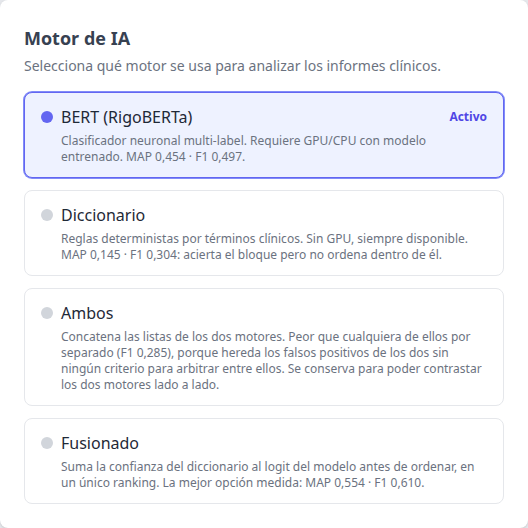
\includegraphics[width=0.7\textwidth]{figs/ui-admin-motor}
\caption{\emph{Backoffice} de administración (\texttt{/admin/settings}): selección del motor de IA entre las cuatro opciones disponibles, aplicable en caliente sin redesplegar.}
\label{fig:admin-settings}
\end{figure}

\paragraph{Selección del modelo desplegado.}
El mismo panel permite además cambiar el \emph{checkpoint} que sirve el clasificador. El motor de IA expone su catálogo en \texttt{GET /admin/models} y acepta cargar otro en caliente con \texttt{POST /admin/models}, sin reiniciar el servicio. El panel consulta ese catálogo al abrirse y presenta cada modelo con su descripción, sus métricas comparables y dos indicadores que conviene distinguir: si está \emph{cargado} y si está \emph{descargado} (Figura~\ref{fig:admin-modelo}). Un modelo del catálogo puede no estar en disco, porque cada \emph{checkpoint} ocupa algo más de 2\,GB y se obtiene por separado con \texttt{make model-download}; sin ese aviso, intentar activarlo fallaría sin explicación, de modo que la acción de carga solo se ofrece sobre los que están presentes.

\begin{figure}[ht]
\centering
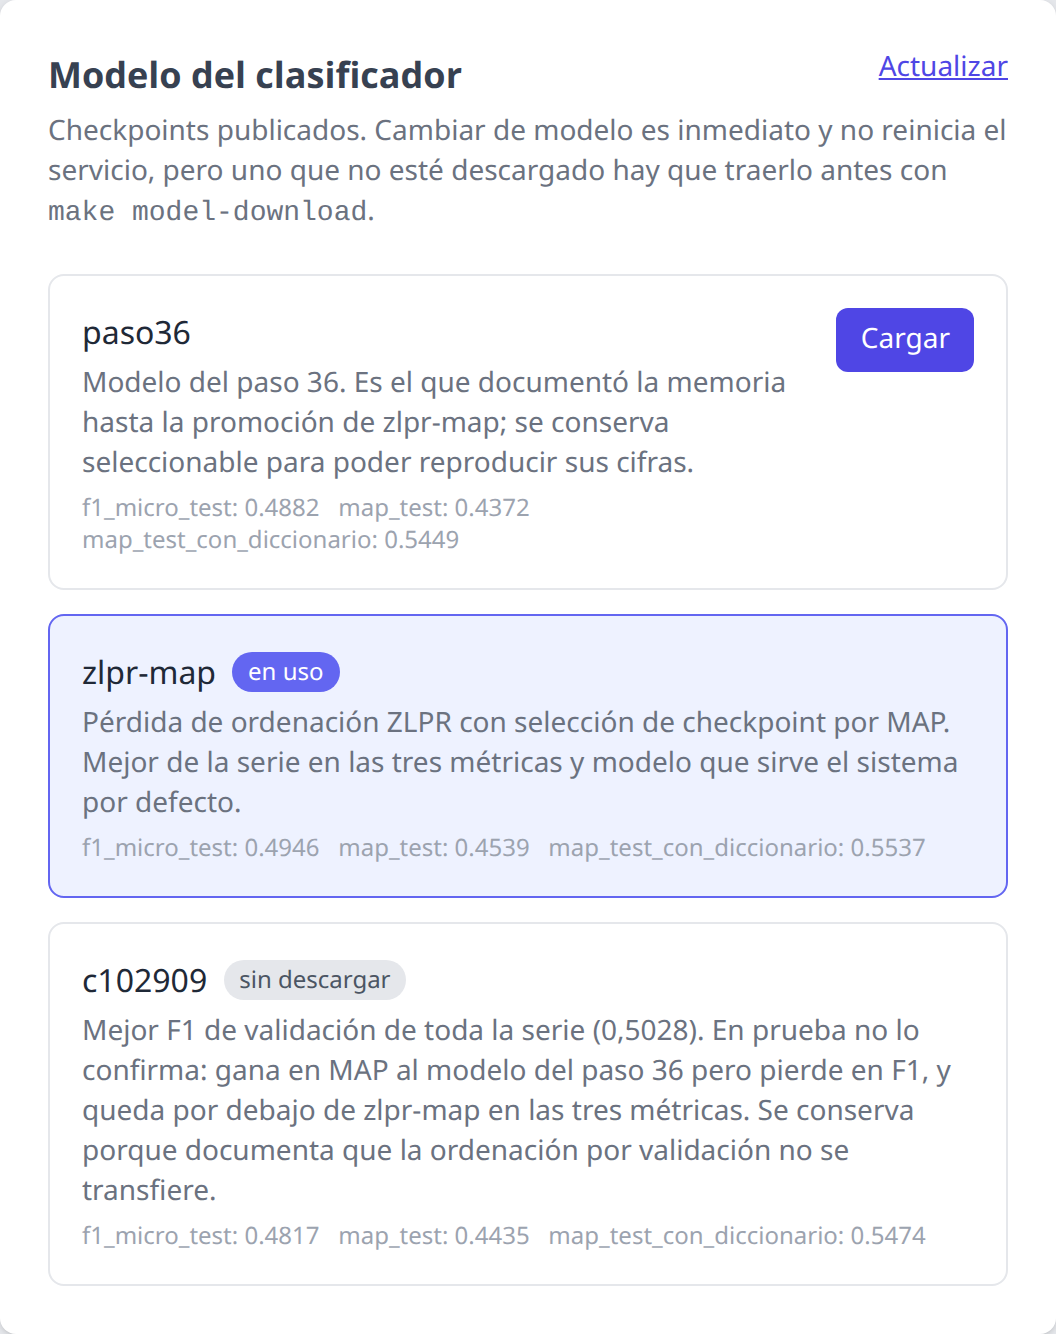
\includegraphics[width=0.65\textwidth]{figs/ui-admin-modelo}
\caption[Selector de modelo del clasificador]{Selector de modelo del clasificador. Cada \emph{checkpoint} muestra sus métricas comparables y dos indicadores independientes: cuál está en uso y cuál está descargado. La acción de carga solo se ofrece sobre los que están presentes en disco.}
\label{fig:admin-modelo}
\end{figure}

La consulta del catálogo se hace de forma tolerante a fallos: si el motor de IA no responde, el panel se abre igualmente y muestra el error en lugar de quedarse en blanco. La razón es práctica, y es la misma que justifica el selector de motores: el panel es justamente donde se cambia de configuración cuando algo va mal, así que no puede depender de que el componente que falla esté disponible.


Esta arquitectura sigue el principio de diseño \emph{«separación de responsabilidades»}: el motor de IA no sabe nada del mecanismo de selección, simplemente atiende la petición que recibe; el backend actúa como orquestador y centraliza la decisión de qué motor invocar; y la interfaz de administración proporciona el punto de control sin acoplarse a la lógica de predicción.

\subsubsection{Representación de la confianza de las predicciones}
\label{sec:confianza-predicciones}

\paragraph{El problema.}
Las probabilidades devueltas por un clasificador multi-label entrenado con \texttt{BCEWithLogitsLoss} son, en general, difíciles de interpretar directamente como porcentajes de confianza. La función de activación \emph{sigmoid} mapea el logit de cada clase al intervalo $(0, 1)$, y durante el entrenamiento el modelo es penalizado por alejarse de los valores objetivo $\{0, 1\}$. Como consecuencia, las predicciones positivas que superan el umbral de decisión tienden a concentrarse en el extremo superior del rango, típicamente entre 0{,}80 y 0{,}99, mientras que las negativas se agrupan cerca de 0. Mostrar este valor directamente al usuario como un porcentaje produce una interfaz poco informativa: casi todos los códigos predichos aparecen con una confianza superior al 90\,\%, lo que impide al codificador clínico priorizar rápidamente los diagnósticos más probables.

\paragraph{Causa raíz.}
El fenómeno es inherente a la calibración del modelo. Un clasificador entrenado únicamente para minimizar la pérdida de entropía cruzada binaria no garantiza que las probabilidades de salida estén calibradas en sentido estadístico~\cite{Guo17}. La solución canónica, \emph{temperature scaling} o calibración de Platt, requeriría un conjunto de validación adicional y añade un hiperparámetro más al ciclo de entrenamiento, lo que excede el alcance de este proyecto.

\paragraph{Solución adoptada: normalización relativa en tiempo de inferencia.}
En lugar de calibrar el modelo, se optó por normalizar las puntuaciones dentro del propio conjunto de predicciones devueltas en cada consulta. Dado un conjunto de $n$ códigos predichos con probabilidades $p_1 \geq p_2 \geq \cdots \geq p_n$, se define la \emph{confianza relativa} de cada código como:

\begin{equation}
 r_i = \frac{p_i - p_n}{p_1 - p_n}, \quad i = 1, \ldots, n
\end{equation}

donde $p_1$ es la probabilidad máxima y $p_n$ la mínima del conjunto. Si todos los valores son iguales ($p_1 = p_n$), se asigna $r_i = 1$ a todos. Este valor $r_i \in [0, 1]$ no representa una probabilidad calibrada, sino la \textbf{fortaleza relativa} de cada predicción respecto a las demás en esa misma consulta.

La normalización se aplica en el servicio de inferencia (\texttt{ai\_engine}) inmediatamente después de construir la lista de predicciones, tanto para el motor BERT como para el clasificador de diccionario, y se incluye en la respuesta como campo \texttt{relative\_confidence} junto a la probabilidad bruta original.

\paragraph{Representación visual.}
En el \emph{frontend}, la confianza relativa se muestra como una barra de progreso de ancho proporcional a $r_i$, con código de color en tres tramos: verde ($r_i \geq 0{,}66$), amarillo ($0{,}33 \leq r_i < 0{,}66$) y naranja ($r_i < 0{,}33$). La probabilidad bruta se conserva visible como texto secundario de pequeño tamaño, de forma que el codificador avanzado pueda consultarla si lo necesita. Esta combinación permite distinguir con rapidez qué códigos tienen mayor respaldo del modelo dentro de cada análisis, sin inducir una falsa precisión numérica.

\subsubsection{Explicabilidad de las predicciones}
\label{sec:explicabilidad}

La explicabilidad (\emph{explainability}) de los sistemas de aprendizaje automático es especialmente relevante en el ámbito clínico, donde el usuario necesita comprender \emph{por qué} el modelo sugiere un determinado código antes de validarlo. Sin esta información, el sistema actúa como una caja negra y dificulta la supervisión médica~\cite{Arrieta20}.

\paragraph{Limitaciones de la atención como explicación.}
Una primera aproximación natural sería utilizar los pesos de atención del transformador: los tokens a los que el mecanismo de atención presta más importancia en la capa final podrían interpretarse como los fragmentos más relevantes del informe. Sin embargo, Jain y Wallace~\cite{Jain19} demostraron empíricamente que los pesos de atención no son explicaciones fiables en el sentido de la teoría de la interpretabilidad: es posible obtener predicciones idénticas con distribuciones de atención muy distintas, y los tokens más atendidos no son necesariamente los responsables de la decisión. Por tanto, aunque los pesos de atención son útiles como herramienta de diagnóstico del modelo, no deben presentarse al usuario final como justificación de las predicciones.

\paragraph{Primera aproximación: Gradient $\times$ Input y su descarte.}
La primera implementación adoptó \textbf{Gradient~$\times$~Input}~\cite{Simonyan14}: para cada código $k$ y token $i$, se calculaba $s_{i,k} = |\nabla_{\mathbf{e}_i}\ell_k \odot \mathbf{e}_i|_1$ mediante una pasada hacia atrás desde el logit del código hasta los embeddings de entrada. El método es post-hoc, no requiere reentrenamiento y tiene coste $O(|\mathcal{P}|)$ pasadas backward para un conjunto de predicciones $\mathcal{P}$.

Sin embargo, la evaluación empírica sobre informes clínicos reales reveló atribuciones de escasa utilidad. En un informe que contenía el término \emph{brucelosis} y para el que el modelo predijo correctamente el código de brucelosis (A23), el método no identificó \emph{brucelosis} entre los tokens de mayor saliencia. Este comportamiento se repitió con otros términos clínicos específicos en las pruebas realizadas: el gradiente al propagarse hacia atrás por las 24 capas del \emph{encoder} RigoBERTa-Clinical se difumina hasta asignar saliencias comparables a términos clínicos y a artículos o preposiciones. El problema es inherente a arquitecturas transformer profundas con pooling en el token \texttt{[CLS]}: el gradiente debe atravesar todos los mecanismos de atención antes de llegar a los embeddings, perdiendo especificidad por el camino.

\paragraph{Método adoptado: atribución por enmascaramiento (\emph{masking perturbation}).}
Descartado el enfoque de gradientes, se adoptó la \textbf{atribución por perturbación}: para cada palabra $w$ del informe y cada código predicho $k$, se mide el descenso en el logit $\ell_k$ al sustituir los tokens de $w$ por el token especial \texttt{[MASK]}:

\begin{equation}
 s_{w,k} = \max\!\left(0,\; \ell_k(\mathbf{x}) - \ell_k(\mathbf{x}_{w \to \text{[MASK]}})\right)
\end{equation}

donde $\mathbf{x}_{w \to \text{[MASK]}}$ es la secuencia de entrada con los tokens de la palabra $w$ reemplazados por \texttt{[MASK]}. Un valor alto de $s_{w,k}$ indica que eliminar $w$ reduce significativamente la confianza del modelo en el código $k$: $w$ es un término clave para esa predicción concreta. Solo se evalúan palabras de cuatro o más caracteres para evitar ruido de stopwords y artículos. Este método mide directamente el \textbf{impacto causal} de cada palabra sobre la predicción, produciendo atribuciones fiables incluso en redes profundas donde los gradientes se difuminan.

La Figura~\ref{fig:ejemplo-explicabilidad} muestra el resultado sobre un informe real del conjunto de prueba, generada con \texttt{ai\_engine/figura\_explicabilidad.py}. El ejemplo sirve para ver a la vez lo que el método consigue y dónde falla: entre los cinco términos que más sostienen el código de dependencia del tabaco aparece \emph{cigarrillos}, que es la evidencia que un codificador buscaría, junto a otras cuatro palabras (\emph{posteriormente}, \emph{micciones}, \emph{persistente}, \emph{normales}) sin relación con ese diagnóstico. La atribución mide una dependencia real del \emph{logit}, no una justificación clínica: si el modelo se apoya en una palabra irrelevante, el método la señala con la misma honestidad con que señala la correcta. Esa es precisamente su utilidad para revisar predicciones, y la razón por la que la interfaz presenta los términos como pistas y no como argumentos.

% Generado por ai_engine/figura_explicabilidad.py: no editar a mano.
\begin{figure}[ht]
\centering
\fbox{\parbox{0.93\textwidth}{\footnotesize\setlength{\baselineskip}{13pt}
Paciente de 70 años de edad, minero jubilado, sin alergias medicamentosas conocidas, que presenta como antecedentes personales: accidente laboral antiguo con fracturas vertebrales y costales; intervenido de enfermedad de Dupuytren en mano derecha y by-pass iliofemoral izquierdo; Diabetes Mellitus tipo II, \colorbox{amarillo!14}{hipercolesterolemia} e hiperuricemia; enolismo activo, fumador de 20 \colorbox{amarillo!45}{cigarrillos} / día. Es derivado desde Atención Primaria por presentar hematuria macroscópica postmiccional en una ocasión y microhematuria \colorbox{amarillo!14}{persistente} \colorbox{amarillo!28}{posteriormente,} con \colorbox{amarillo!28}{micciones} \colorbox{amarillo!14}{normales.} En la exploración física presenta un buen estado general, con abdomen y genitales \colorbox{amarillo!14}{normales;} tacto rectal compatible con
}}
\caption[Ejemplo de explicabilidad sobre un informe real]{Términos que sostienen la predicción
del código \texttt{F17.210} (Dependencia de nicotina, cigarrillos, sin complicaciones) sobre un informe del conjunto de
prueba. El sombreado es proporcional a la caída del \emph{logit} al enmascarar cada palabra,
en tres niveles. Los cinco primeros: \emph{cigarrillos} (0,41), \emph{posteriormente} (0,16), \emph{micciones} (0,14), \emph{persistente} (0,12), \emph{normales} (0,11).}
\label{fig:ejemplo-explicabilidad}
\end{figure}


\paragraph{Implementación.}
La atribución se calcula en el método \texttt{CIE10Classifier.explain()} (\texttt{ai\_engine/classifier.py}):

\begin{enumerate}
 \item Se tokeniza el texto y se obtiene el mapeo palabra~$\to$~posiciones de subword tokens mediante \texttt{word\_ids()} del tokenizador.
 \item Se ejecuta una pasada \emph{forward} de referencia para obtener los logits originales $\ell_k(\mathbf{x})$ de todos los códigos predichos.
 \item Para cada palabra candidata se construye una versión enmascarada de la secuencia sustituyendo sus tokens por \texttt{[MASK]}.
 \item Las versiones enmascaradas se agrupan en \emph{batches} de 16 y se procesan en una única pasada \emph{forward} por batch, obteniendo $\ell_k(\mathbf{x}_{w \to \text{[MASK]}})$ para todos los códigos simultáneamente.
 \item Se calcula $s_{w,k}$ para cada par (palabra, código) y se devuelven las $k$ palabras de mayor importancia por código.
\end{enumerate}

El coste es $O(\lceil|W|/B\rceil)$ pasadas \emph{forward} adicionales, donde $|W|$ es el número de palabras candidatas y $B = 16$ el tamaño de \emph{batch}. Con informes de CodiEsp esto supone en torno a 128 evaluaciones por consulta, y resultó ser el componente que domina por completo la latencia del sistema.

\paragraph{El coste de explicar, medido.}
La medición sobre 30 informes del conjunto de prueba separa dos costes de orden distinto. Proponer los códigos de un informe cuesta 0{,}331~s de mediana y 0{,}340~s en el percentil 95 sobre el AMD Ryzen 9 7900X del equipo de desarrollo, y 0{,}017~s sobre su NVIDIA RTX 4080. Justificarlos con el método exhaustivo cuesta 55{,}1~s en esa misma CPU (tabla~\ref{tab:explicabilidad}), más de dos órdenes de magnitud por encima. Dicho de otro modo, el 99~\% del tiempo que esperaba el usuario no se dedicaba a decidir los códigos sino a justificarlos.

La Tabla~\ref{tab:latencia} desglosa el ciclo completo con el método finalmente adoptado, que es lo que un usuario espera de principio a fin. Interesa verlo junto y no solo por partes, porque las dos peticiones se encadenan: la de atribución no se lanza hasta que llegan los códigos.

\begin{table}[h]
\centering
\small
\caption[Latencia del ciclo completo por informe, con el método de atribución adoptado]{Latencia del ciclo completo por informe, con el método de atribución adoptado. Predicción medida con \texttt{make ai-bench-predict} (\texttt{ai\_engine/bench\_predict.py}) sobre 30 informes del conjunto de prueba; atribución con \texttt{make ai-bench-explain} y su variante \texttt{DEVICE=cuda} (Tablas~\ref{tab:explicabilidad} y~\ref{tab:explain-diccionario}). CPU: AMD Ryzen 9 7900X. GPU: NVIDIA RTX 4080.}
\label{tab:latencia}
\begin{tabular}{lrr}
\hline
\textbf{Fase} & \textbf{CPU (s)} & \textbf{GPU (s)} \\
\hline
Proponer los códigos (\texttt{/predict})   & 0{,}331 & 0{,}017 \\
Justificarlos (\texttt{/explain})          & 16{,}2  & 0{,}51  \\
\hline
\textbf{Ciclo completo}                    & \textbf{16{,}5} & \textbf{0{,}53} \\
\hline
\end{tabular}

\vspace{2mm}
{\footnotesize El total es la suma de las dos peticiones, que el cliente encadena, y no una medición de extremo a extremo: no incluye el tránsito por el backend ni por el canal WebSocket. La fila de atribución recoge el filtro por gradiente con 32 candidatos; la variante adoptada lo siembra además con los términos del diccionario, con coste equivalente (0{,}51~s en GPU, Tabla~\ref{tab:explain-diccionario}). Lo que el codificador clínico percibe no es el total, sino la primera fila: los códigos aparecen en cuanto están y los términos se incorporan después.}
\end{table}

Las mediciones descartan la primera inferencia, y conviene justificar por qué no es una forma de maquillar el resultado. Esa primera pasada paga costes que se abonan una sola vez por proceso: la reserva inicial de memoria del \emph{backend} de \emph{torch} y, cuando hay acelerador, la creación del contexto CUDA y la elección de los núcleos de cálculo para cada forma de tensor. Ninguno de ellos lo sufre un usuario, porque el motor carga el modelo al arrancar el contenedor y permanece en memoria entre peticiones. Su peso, además, está medido: en CPU la primera predicción cuesta 0{,}364~s frente a los 0{,}331~s de la mediana, una diferencia despreciable, mientras que en GPU son 0{,}146~s frente a 0{,}017~s, ocho veces más. Es decir, descartarla solo cambia algo en la columna de GPU, y allí lo que evita es atribuir a cada informe un coste de arranque que se produce una única vez.

Ese diagnóstico admite dos respuestas independientes, y se aplicaron las dos.

\paragraph{Separar la explicación de la predicción.}
La primera es de diseño de la interacción y no del algoritmo. La atribución se desacopla en un \emph{endpoint} propio, de modo que la predicción devuelve los códigos en cuanto están y las palabras que los justifican llegan en una segunda petición. El orden en que el usuario consume la información lo permite: primero lee la lista de códigos propuestos y solo después despliega uno concreto para saber por qué se ha sugerido, de manera que esperar a la atribución antes de mostrar nada era hacerle esperar por algo que todavía no estaba mirando.

Esta separación tiene además un efecto que no es evidente. En el modo que fusiona ambos motores, los términos del diccionario \emph{ya están calculados} cuando se responde, porque la coincidencia por expresiones regulares se ejecutó para construir la bonificación. La interfaz puede así mostrar de inmediato la evidencia léxica, que es literal y la más convincente para un profesional, y completar después con las palabras del modelo, señalando entre tanto que faltan. La explicación deja de ser una operación de todo o nada.

\paragraph{Abaratar la atribución: tres estrategias medidas.}
La segunda respuesta ataca el propio cálculo. Se implementaron tres estrategias como versiones sucesivas de la misma funcionalidad, seleccionables en tiempo de ejecución y conservando siempre la original como referencia. Las tres devuelven palabras medidas por enmascarado real: lo que cambia entre ellas es a cuántas palabras se pregunta, no cómo se mide a las que se pregunta, de modo que pueden intercambiarse sin alterar la interpretación de la salida. La Tabla~\ref{tab:explicabilidad} recoge su coste y su fidelidad.

\begin{table}[h]
\centering
\small
\caption[Estrategias de atribución sobre informes de CodiEsp]{Estrategias de atribución sobre informes de CodiEsp. La fidelidad se mide contra el método exhaustivo, que es la referencia por construcción. Generada con \texttt{make ai-bench-explain} y su variante \texttt{DEVICE=cuda} (\texttt{ai\_engine/bench\_explain.py}). CPU: AMD Ryzen 9 7900X. GPU: NVIDIA RTX 4080.}
\label{tab:explicabilidad}
\begin{tabular}{lrrrr}
\hline
\textbf{Estrategia} & \textbf{CPU (s)} & \textbf{GPU (s)} & \textbf{Solape@5} & \textbf{Término principal} \\
\hline
Exhaustiva (referencia) & 55{,}1 & 1{,}79 & 1{,}00 & 1{,}00 \\
Poda por grupos & 92{,}4 & 3{,}05 & 0{,}96 & 0{,}97 \\
\hline
Gradiente, 16 candidatos & 9{,}3 & 0{,}30 & 0{,}66 & 0{,}77 \\
Gradiente, 32 candidatos & \textbf{16{,}2} & \textbf{0{,}51} & \textbf{0{,}83} & \textbf{0{,}97} \\
Gradiente, 64 candidatos & 30{,}4 & 0{,}95 & 0{,}91 & 0{,}97 \\
Gradiente, 96 candidatos & 44{,}1 & 1{,}36 & 0{,}96 & 1{,}00 \\
\hline
Diccionario & 0{,}7 & n/a & 0{,}09 & 0{,}23 \\
\hline
\end{tabular}

\vspace{2mm}
{\footnotesize Cada columna de tiempos procede de una única ejecución sobre los mismos seis informes, de modo que las filas son comparables entre sí. La fidelidad es idéntica en ambos dispositivos, como corresponde al mismo algoritmo. El diccionario no consulta el \emph{encoder}, de modo que su tiempo no depende del acelerador y se omite esa medición. El método de diccionario no consulta el \emph{encoder}: devuelve las frases que hicieron coincidencia, lo que explica a la vez que sea dos órdenes de magnitud más rápido y que apenas coincida con la referencia. No es una aproximación barata de la atribución del modelo, sino otro tipo de evidencia.}
\end{table}

La columna de GPU obliga a matizar la conclusión de este apartado. En la máquina de desarrollo sin acelerador, el método exhaustivo tarda 55~s por informe y de ahí que la atribución tenga que resolverse en una petición aparte. Sobre la RTX~4080 ese mismo método baja a 1,79~s, un factor de 31, y el conjunto de estrategias rápidas queda por debajo del segundo y medio. Es decir, el coste que motiva toda la ingeniería de este apartado no es una propiedad del método de atribución sino del hardware sobre el que se ejecuta: con un acelerador, la variante más fiel sería utilizable en línea y las aproximaciones dejarían de hacer falta. La arquitectura elegida sigue siendo la adecuada, porque el sistema debe poder servirse sin acelerador: el modo CPU es un escenario de despliegue soportado (Anexo~\ref{cap:AnexoK}) y la atribución es justo lo que deja de ser viable en él. Conviene declarar, eso sí, que se trata de una decisión condicionada por esa restricción y no por el algoritmo: donde hay GPU, la variante más fiel sería utilizable en línea.

\paragraph{Dos fallos que solo aparecen con la tarjeta visible.}
Servir sobre la GPU destapó dos defectos que el modo CPU ocultaba, y ambos merecen mención porque ilustran que un servicio que responde no es un servicio correcto. El primero afectaba al lematizador del diccionario: \texttt{spaCy} se cargaba con \texttt{prefer\_gpu} y su \emph{pipeline} quedaba repartido entre dispositivos, de modo que el motor fusionado fallaba entero con un error de tensores en dispositivos distintos. Se fija a CPU a propósito, porque ese componente no consulta el \emph{encoder} y no gana nada con el acelerador. El segundo es de concurrencia y estaba presente también en CPU, aunque allí resultaba más difícil de provocar: el filtro por gradiente registra un \emph{hook} sobre la capa de embeddings, que es única para todo el proceso, y mientras está puesto cualquier otra pasada hacia delante lo dispara. Una predicción concurrente entra bajo \texttt{no\_grad} y el \texttt{retain\_grad} del \emph{hook} la abortaba con un error del servidor: analizar un informe mientras se explicaba otro devolvía un fallo a un usuario que no había pedido ninguna explicación. Se corrige con una guarda en el \emph{hook} y un cerrojo que serializa únicamente el tramo con \emph{hook}, de modo que las predicciones siguen atendiéndose en paralelo. Ambos casos quedan fijados con pruebas que fallan sin la corrección.

La \textbf{poda por grupos} enmascara conjuntos de palabras y descarta entero el conjunto que no altera ningún \emph{logit}, partiendo por la mitad solo los que sí lo hacen. La hipótesis era que la importancia fuese lo bastante dispersa como para descartar subárboles completos, y resultó falsa: es un 73~\% más lenta que el método al que pretendía mejorar. La razón es aritmética y no de implementación. Un árbol binario sobre $n$ palabras tiene $2n-1$ nodos, así que sin poda cuesta el doble que preguntar una por una; solo compensa si con $m$ palabras relevantes de $n$ el recorrido se reduce a unas $2m\log_2(n/m)$ evaluaciones, que con $n \approx 128$ y $m = 5$ serían 47. Una medición directa de la dispersión lo confirma: un informe aporta unas 147 palabras candidatas y, con el umbral de poda por defecto, el 71,9~\% mueve el \emph{logit} por encima del corte, de modo que la poda casi nunca dispara.

Cabía pensar que el problema fuese el umbral y no el método. No lo es. Subirlo acelera pero se lleva la fidelidad por delante: con 0,25 el coste iguala al del exhaustivo y el solape cae a 0,77; con 0,50 baja a 0,61. La comparación que zanja el asunto es con el filtro por gradiente, que con 96 candidatos alcanza el mismo solape de 0,96 en menos de la mitad de tiempo. A igualdad de fidelidad resulta más barato y a igualdad de coste resulta más fiel, de modo que la poda por grupos queda \textbf{dominada en todos los puntos de operación}. Se conserva documentada como resultado negativo, y seguiría teniendo sentido en un corpus donde la importancia estuviera concentrada en unas pocas palabras, que es la condición que aquí no se cumple.

\paragraph{Una vía que sí salió: sembrar el filtro con el diccionario.}
El filtro por gradiente decide a qué treinta y dos palabras preguntar basándose únicamente en la saliencia. Pero el sistema ya dispone de otra fuente de evidencia sobre el mismo texto: el diccionario de patrones reconoce frases clínicas que se sabe asociadas a códigos concretos. Esas palabras se verifican ahora siempre, ocupen o no los primeros puestos de la saliencia, y el gradiente reparte el presupuesto restante. El emparejamiento se hace palabra a palabra y es deliberadamente generoso, porque verificar una de más cuesta una pasada del \emph{encoder} y dejar fuera la que justifica el código cuesta una explicación incompleta.

\begin{table}[h]
\centering
\small
\caption{Efecto de sembrar el filtro por gradiente con los términos del diccionario. Medido con \texttt{make ai-bench-explain DEVICE=cuda} sobre los mismos informes.}
\label{tab:explain-diccionario}
\begin{tabular}{lrrr}
\hline
\textbf{Variante} & \textbf{Segundos} & \textbf{Solape@5} & \textbf{Término principal} \\
\hline
Gradiente, 32 candidatos & 0{,}52 & 0{,}83 & 0{,}97 \\
\rowcolor{gray!15}
\textbf{Gradiente, 32 candidatos + diccionario} & \textbf{0{,}51} & \textbf{0{,}87} & \textbf{1{,}00} \\
Gradiente, 64 candidatos & 0{,}96 & 0{,}91 & 0{,}97 \\
\hline
\end{tabular}
\end{table}

La ganancia es pequeña pero gratuita (Tabla~\ref{tab:explain-diccionario}): mismo coste, cuatro puntos más de solape con el método exhaustivo y, sobre todo, el término que encabeza la explicación coincide ahora con el de la referencia en el cien por cien de los casos, frente al noventa y siete anterior. Conseguir esa fidelidad solo con el gradiente exigiría doblar el presupuesto a sesenta y cuatro candidatos y pagar el doble de tiempo. El resultado tiene además una lectura que va más allá de la optimización: las dos fuentes de evidencia que se complementaban en la predicción, el clasificador y el diccionario, también se complementan al explicarla.

\paragraph{Una vía que tampoco salió: filtrar las palabras vacías.}
El conjunto de candidatas se construye descartando las palabras de menos de cuatro caracteres, de modo que preposiciones y pronombres largos («durante», «mediante», «cuando») siguen entrando y consumen presupuesto de verificación. Parecía una mejora evidente, y se midió antes de darla por buena. No lo fue: añadir una lista de palabras vacías reduce el coste del método exhaustivo un 5\,\% y el del método por defecto apenas un 2\,\%, sin cambio apreciable en la fidelidad. La comprobación que cerró la cuestión fue otra: sobre doce informes y ciento setenta y cinco términos, \textbf{ninguna palabra vacía llegaba nunca a los cinco primeros}, ni siquiera sin el filtro. El modelo no se apoyaba en ellas, así que no había tampoco una mejora de calidad que las métricas de coste no estuvieran capturando. La mejora era residual y el cambio se revirtió: una lista de palabras codificada a mano tiene un coste de mantenimiento y un riesgo de descartar algún término que en un informe concreto sí importe, y ninguno de los dos se paga con un 2\,\%.

El \textbf{filtrado por gradiente} sí funciona. Una única pasada hacia atrás ordena las palabras candidatas y solo se enmascaran de verdad las más prometedoras, lo que reduce el coste a una cuarta parte. La objeción que llevó a descartar Gradient~$\times$~Input como método de atribución no se aplica aquí, porque el gradiente no responde sino que solo decide a quién se pregunta: cualquier error de orden que cometa lo corrige después la medición por enmascarado. El Algoritmo~\ref{alg:atribucion} detalla el procedimiento.

\begin{algorithm}[ht]
\DontPrintSemicolon
\caption{Atribución por enmascarado con filtro de gradiente.}
\label{alg:atribucion}
\KwIn{informe $x$; códigos predichos $K$; presupuesto $m=32$; palabras prioritarias $W_\pi$ (las que el diccionario ya ha detectado)}
\KwOut{importancia $s_{w,k}$ de cada palabra verificada $w$ para cada código $k \in K$}
$W \leftarrow$ palabras de $x$ con al menos cuatro caracteres\;
$\ell^{0} \leftarrow$ logits del modelo sobre $x$\;
$g \leftarrow$ gradiente de $\sum_{k \in K}\ell_k$ respecto de los \emph{embeddings} de entrada (una pasada hacia atrás)\;
\ForEach{palabra $w \in W$}{
  $\sigma_w \leftarrow \sum_{t \in w}\lvert\langle g_t, e_t\rangle\rvert$, con $e_t$ el \emph{embedding} del \emph{token} $t$\;
}
$V \leftarrow$ las palabras de $W \cap W_\pi$ seguidas del resto de $W$ ordenado por $\sigma_w$ decreciente, recortada a $m$ palabras\;
\ForEach{palabra $w \in V$}{
  $s_{w,k} \leftarrow \max\!\left(0,\ \ell^{0}_k - \ell_k(x_{w \to \text{[MASK]}})\right)$ para todo $k \in K$\;
}
\Return{$s$}\;
\end{algorithm}

Conviene ser preciso sobre qué error puede cometer esta estrategia, porque no todos cuestan lo mismo ante un profesional. \emph{No puede inventar}: todo término que reporta tiene una caída de \emph{logit} medida, luego influye de verdad en la predicción. Lo que sí puede es dejarse fuera la palabra más importante, porque nunca llega a preguntarle, en cuyo caso se muestra un término real pero no el más fuerte. El error es unidireccional, y está cuantificado: el término principal coincide con el del método exhaustivo en el 97~\% de los casos. La distinción importa porque un término falso destruiría la confianza del codificador clínico en la herramienta, mientras que un término real pero subóptimo es una explicación peor, no una explicación engañosa.

El número de candidatos que se verifican fija el compromiso, y el barrido muestra que existe un codo claro. Con 16 la estrategia se rompe: el término principal deja de coincidir una de cada cuatro veces, que es precisamente el error que un profesional notaría. Con 64 se paga el doble de tiempo a cambio de ocho puntos de solape, y con 96 la ventaja sobre el método exhaustivo prácticamente desaparece. El valor adoptado, 32, conserva el término principal en el 97~\% de los casos por una fracción del coste.

Ninguna de las estrategias baja de los siete segundos, lo que confirma que la optimización algorítmica no basta por sí sola: lo que resuelve el problema de interacción es la separación en dos peticiones, y las estrategias mejoran el coste dentro de esa separación.

El administrador elige la estrategia desde el \emph{backoffice} (Figura~\ref{fig:admin-explicabilidad}). El cambio se aplica a las siguientes explicaciones sin redesplegar, porque el backend envía la estrategia vigente como parámetro \texttt{method} en cada petición a \texttt{/explain}, y se guarda en la base de datos para que sobreviva a un reinicio.

\begin{figure}[ht]
\centering
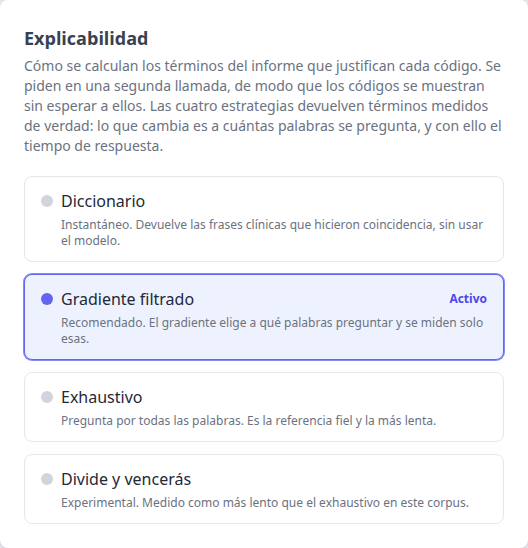
\includegraphics[width=0.6\textwidth]{figs/ui-admin-explicabilidad}
\caption{\emph{Backoffice} de administración: selección de la estrategia de atribución de términos (diccionario, gradiente filtrado, exhaustivo o divide y vencerás). Está activo el gradiente filtrado, que es el que sirve el sistema.}
\label{fig:admin-explicabilidad}
\end{figure}

\paragraph{El diccionario como explicación inmediata.}
Queda una cuarta vía que no consume el \emph{encoder} en absoluto: devolver las frases clínicas que hicieron coincidencia por expresión regular. Responde en 0{,}58~s, ochenta y tres veces más rápido que el método exhaustivo, y en el motor fusionado esos términos ya están calculados cuando se responde a la predicción, porque la coincidencia se ejecutó para ordenar los códigos.

Sus dos límites también están medidos. Cubre el 63~\% de los códigos propuestos: cuando el bloque no ha hecho coincidencia, ese código se queda sin justificación léxica. Y solo el 15~\% de las palabras que el modelo considera importantes aparece dentro de las frases que encuentra el diccionario, de modo que ambas fuentes señalan evidencias distintas en el 85~\% de los casos.

Esa última cifra es la que justifica mostrar las dos y no elegir una. Si coincidieran, bastaría con la barata; al ser mayoritariamente complementarias, cada una aporta información que la otra no tiene, y el codificador clínico dispone de dos justificaciones independientes de la misma propuesta. Conviene subrayar que no compiten en la misma tarea: el diccionario explica por qué el informe apunta a ese bloque, con frases literales, y el modelo explica qué palabras sostienen el código concreto dentro del bloque. Compararlas con la misma métrica produciría un número bajo que se leería como que el diccionario explica peor, cuando lo que hace es explicar otra cosa.

\paragraph{Clasificador de diccionario.}
Para el motor basado en reglas, la explicabilidad es directa e inherente al diseño: el clasificador devuelve los términos clínicos concretos del informe que activaron cada código (\texttt{matched\_terms}), extraídos mediante las expresiones regulares construidas con spaCy. Estos términos se presentan al usuario de la misma forma que los triggers del motor BERT.

\paragraph{Representación visual.}
Los términos de cada código se presentan como \emph{chips} bajo su descripción, y el color distingue su procedencia: los que provienen del diccionario son coincidencias literales del informe y los del modelo son las palabras cuya eliminación más reduce el \emph{logit}. Son evidencias de distinta naturaleza, así que la interfaz las etiqueta en lugar de fundirlas en una única lista ordenada, y una nota emergente explica de dónde sale cada una. Cuando las palabras del modelo aún se están calculando, la tarjeta muestra los términos léxicos que ya tiene junto a un indicador de progreso, en lugar de dejar el espacio vacío.

\paragraph{Trabajo futuro.}
Una extensión natural es la estimación de intervalos de confianza en las atribuciones mediante múltiples perturbaciones con ruido (\emph{SmoothGrad}~\cite{Smilkov17}), o el uso de \emph{SHAP KernelExplainer}~\cite{Lundberg17} para obtener valores de Shapley con garantías de equidad en la distribución de la importancia entre palabras. Ambos métodos añaden coste computacional pero proporcionan propiedades teóricas más sólidas.

\subsection{Autenticación y seguridad}
\label{sec:seguridad}

El sistema implementa autenticación mediante registro con confirmación por email. Al registrarse, el usuario recibe un email con un enlace de confirmación generado con \texttt{Phoenix.Token}. Una vez confirmada la cuenta, el inicio de sesión devuelve un token Bearer que el frontend almacena en \texttt{localStorage} y envía en la cabecera \texttt{Authorization} de cada petición REST y en el \emph{handshake} del WebSocket. El \emph{plug} \texttt{RequireAuth} verifica el token en todas las rutas protegidas. Los tokens tienen una validez de \textbf{una hora} (\texttt{max\_age: 3\_600}); pasado ese tiempo, cualquier petición es rechazada con un error 401, lo que limita la ventana de exposición ante un robo de sesión. La Figura~\ref{fig:auth-flujo} resume el flujo de autenticación completo.

\begin{figure}[ht]
\centering
\resizebox{0.9\textwidth}{!}{
\begin{tikzpicture}[
  every node/.style={font=\small\sffamily},
  paso/.style={draw=aquaESI!80, fill=aquaESI!12, thick, rectangle, rounded corners=3pt,
              minimum width=10.5cm, minimum height=0.95cm, align=center},
  mail/.style={draw=ocre!80, fill=ocre!15, thick, rectangle, rounded corners=3pt,
               minimum width=10.5cm, minimum height=0.95cm, align=center},
  chk/.style={draw=turquesa!80, fill=turquesa!15, thick, rectangle, rounded corners=3pt,
              minimum width=10.5cm, minimum height=0.95cm, align=center},
  arr/.style={->, >=Stealth, thick},
  node distance=0.55cm,
]
\node[paso] (reg) {1. Registro: \texttt{POST /auth/register} (contraseña con \emph{hash} bcrypt)};
\node[mail, below=of reg] (mail) {2. Correo de confirmación con enlace firmado (\texttt{Phoenix.Token})};
\node[paso, below=of mail] (conf) {3. Confirmación: \texttt{GET /auth/confirm/:token} $\rightarrow$ cuenta activada};
\node[paso, below=of conf] (login) {4. Inicio de sesión: \texttt{POST /auth/login} $\rightarrow$ \{user, token Bearer\} (validez 1\,h)};
\node[paso, below=of login] (use) {5. Peticiones autenticadas: \texttt{Authorization: Bearer} en REST y en el \emph{handshake} WebSocket};
\node[chk, below=of use] (auth) {6. \texttt{RequireAuth} verifica el token (\texttt{Phoenix.Token.verify}, \texttt{max\_age=3600}); si no, HTTP 401};

\draw[arr] (reg) -- (mail);
\draw[arr] (mail) -- (conf);
\draw[arr] (conf) -- (login);
\draw[arr] (login) -- (use);
\draw[arr] (use) -- (auth);
\end{tikzpicture}
}
\caption{Flujo de autenticación: del registro con confirmación por correo a la verificación del token \emph{Bearer} (\texttt{Phoenix.Token}, validez de una hora) en cada petición REST y en el \emph{handshake} del WebSocket.}
\label{fig:auth-flujo}
\end{figure}

Las contraseñas se almacenan hasheadas con bcrypt y se exige una longitud mínima de \textbf{12 caracteres} para reducir la vulnerabilidad ante ataques de fuerza bruta. El servicio de email se implementa con Swoosh y, en el entorno de desarrollo, se captura con Mailpit (accesible en \texttt{http://localhost:8025}).

La política CORS del backend se gestiona mediante el \emph{plug} \texttt{CORSPlug} en el \emph{endpoint} Phoenix. Los orígenes permitidos se leen en tiempo de ejecución desde la variable de entorno \texttt{CORS\_ORIGINS}, lo que permite restringir el acceso a los dominios exactos del frontend sin modificar el código. Los métodos permitidos son \texttt{GET}, \texttt{POST}, \texttt{PUT}, \texttt{DELETE} y \texttt{OPTIONS}; las cabeceras autorizadas son \texttt{Authorization}, \texttt{Content-Type} y \texttt{Accept}. En producción, \texttt{CORS\_ORIGINS} se establece al dominio \texttt{clicoder.app}, de modo que cualquier petición cruzada desde un origen distinto es rechazada antes de llegar a la lógica de la aplicación.

\subsubsection{Limitación de peticiones (\emph{rate limiting})}

Los \emph{endpoints} de autenticación (\texttt{POST /auth/register}, \texttt{POST /auth/login} y \texttt{GET /auth/confirm/:token}) están protegidos por un mecanismo de limitación de peticiones implementado mediante una tabla ETS (\emph{Erlang Term Storage}) local, sin dependencias externas. El \emph{plug} \texttt{AppWeb.Plugs.RateLimit} mantiene una ventana deslizante de 60 segundos por dirección IP: si la misma IP supera las 10 peticiones en ese intervalo, el servidor responde con el código HTTP 429 (\emph{Too Many Requests}) antes de ejecutar cualquier lógica de negocio. Este límite dificulta los ataques de fuerza bruta sobre el formulario de inicio de sesión sin necesitar infraestructura adicional.

\subsubsection{Cabeceras de seguridad HTTP}

El \emph{endpoint} Phoenix incluye el \emph{plug} \texttt{put\_security\_headers}, que añade a todas las respuestas un conjunto de cabeceras defensivas:

\begin{itemize}
 \item \texttt{X-Frame-Options: DENY} impide que la aplicación sea embebida en un \texttt{<iframe>}, previniendo ataques de \emph{clickjacking}.
 \item \texttt{X-Content-Type-Options: nosniff} fuerza al navegador a respetar el tipo MIME declarado, evitando la ejecución involuntaria de recursos mal tipificados.
 \item \texttt{Referrer-Policy: strict-origin-when-cross-origin} limita la información del \emph{referer} enviada en peticiones cruzadas, reduciendo la filtración de URLs internas.
 \item \texttt{Strict-Transport-Security: max-age=31536000; includeSubDomains} (HSTS) obliga al navegador a usar HTTPS durante un año para el dominio y todos sus subdominios, eliminando la posibilidad de ataques de degradación de protocolo (\emph{SSL stripping}).
\end{itemize}

\subsubsection{Auditoría de dependencias}

Un sistema que trata datos de salud hereda las vulnerabilidades de todo lo que importa, no solo las de su propio código, así que las tres bases de código se auditan por separado: \texttt{make audit-backend} (\texttt{mix hex.audit} sobre Elixir), \texttt{make audit-js} (\texttt{npm audit} sobre el frontend) y \texttt{make audit-python} (\texttt{pip-audit} sobre el motor de IA), agrupados bajo \texttt{make audit}. Elixir no tiene paquetes retirados ni vulnerables. El frontend partía de diecisiete avisos; \texttt{npm audit fix} resolvió catorce sin subir ninguna dependencia de versión mayor, y las tres restantes están en \texttt{@vitest/mocker}, herramienta de pruebas que no llega al navegador y para la que no hay parche publicado todavía. El motor de IA tiene un aviso sin arreglo publicado en \texttt{diskcache} (\texttt{PYSEC-2026-2447\allowbreak}): deserializa con \texttt{pickle} por defecto, lo que permite ejecución de código si un atacante consigue escritura en el directorio de caché. Es dependencia transitiva de \texttt{llama\_cpp\_python} (el motor del resumidor LLM, sección~\ref{sec:resumidor}), pero solo a través de la clase \texttt{LlamaDiskCache}, que ningún módulo propio instancia: el resumidor usa la caché en memoria por defecto de la biblioteca, de modo que el código que ejercitaría la vulnerabilidad no llega a ejecutarse aunque el resumidor esté activo.

\subsection{Observabilidad}
\label{sec:observabilidad}

Un prototipo desplegado y en uso necesita responder a dos preguntas distintas: si algo se ha roto, y si el sistema se está comportando como se espera. Se resuelven con dos mecanismos separados.

\textbf{Seguimiento de errores con Sentry}. El backend y el motor de IA envían sus excepciones no controladas a Sentry, cada uno con su propio DSN (\texttt{SENTRY\_DSN} y \texttt{SENTRY\_DSN\_AI}), de modo que un fallo del servicio de inferencia no se confunde con uno de la capa de aplicación. En Elixir la integración se registra en el \emph{endpoint} de Phoenix y captura además los errores de los procesos supervisados, que de otro modo se perderían en el reinicio del árbol de supervisión. En Python las excepciones de las peticiones se capturan con las integraciones de FastAPI y Starlette, y los fallos de carga del modelo se notifican explícitamente con \texttt{sentry\_sdk.capture\_exception}, porque un arranque degradado no lanza ninguna excepción hacia el cliente y pasaría inadvertido. Lo que importa aquí no es tener la herramienta, sino que un error en producción llega con el rastro de pila y el contexto de la petición sin depender de que alguien mire los registros: ese contexto es también lo que obliga al filtrado descrito a continuación.

\textbf{Métricas con Prometheus y Grafana}. El motor de IA expone \texttt{GET /metrics} con la latencia de inferencia por motor y el estado de carga de cada modelo; el backend publica las suyas en el puerto 9568. Prometheus las recoge junto a las del anfitrión, los contenedores y el proxy, y una sonda \emph{blackbox} comprueba desde fuera que los tres servicios responden. Grafana los presenta en paneles aprovisionados desde el repositorio (Anexo~\ref{cap:AnexoK}). La distinción con Sentry es deliberada: Sentry dice qué ha fallado, las métricas dicen si está fallando algo que todavía nadie ha notado.

\subsubsection{Filtrado de datos sensibles en el sistema de monitorización}

Un aviso de error viaja a un servicio de terceros, de modo que todo lo que se adjunte al aviso sale del sistema. Eso convierte a la monitorización en el punto por el que los datos pueden escaparse sin que nadie lo note, porque el sistema sigue funcionando igual mientras filtra. El criterio adoptado es que hacia fuera solo salgan \textbf{identificadores}, nunca contenido: con el identificador de la conversación y el del usuario, el error se investiga consultando la base de datos local; el informe clínico, el correo y la dirección IP no aportan nada para depurar y son precisamente lo que no puede salir.

En el backend, el \emph{callback} \texttt{before\_send} del módulo \texttt{AppWeb.SentryFilter} interviene cada evento antes de enviarlo. Sustituye por \texttt{[FILTERED]} los campos sensibles del cuerpo de la petición, recorriendo también los mapas anidados: \texttt{password}, \texttt{password\_hash}, \texttt{token}, \texttt{content} (texto del informe), \texttt{report\_text}, \texttt{authorization} y \texttt{cookie}. A esos se añaden tres piezas que el filtrado por nombre de campo no cubría:

\begin{itemize}
 \item La \textbf{cadena de consulta} completa, porque por ahí viaja el token de confirmación de correo (\texttt{GET /auth/confirm/:token}), que da acceso a la cuenta.
 \item La \textbf{dirección IP} del cliente, tanto en \texttt{REMOTE\_ADDR} como en las cabeceras \texttt{X-Forwarded-For} y \texttt{X-Real-IP}. Es dato personal del artículo~4 del RGPD.
 \item Los \textbf{datos del usuario} adjuntos al evento, de los que solo se conserva el identificador de la base de datos.
\end{itemize}

En el motor de inteligencia artificial el riesgo era mayor y de otra naturaleza, porque este servicio recibe el informe clínico en el cuerpo de cada petición. El SDK de Python adjunta por omisión \textbf{las variables locales de cada marco de la pila}, de modo que una excepción durante una predicción habría enviado el texto del informe íntegro: la variable que lo contiene es un argumento de la función que estaba ejecutándose. Se desactiva explícitamente con \texttt{include\_local\_variables}, junto a \texttt{send\_default\_pii} y \texttt{max\_request\_body\_size}, que impiden respectivamente el envío de datos identificativos y del cuerpo de la petición.

Este filtrado no es una capa opcional de endurecimiento sino parte del cumplimiento descrito en la sección~\ref{sec:rgpd}, de modo que se fija con pruebas (\texttt{backend/test/app\_web/sentry\_filter\_test.exs}): comprueban que el informe no sale ni anidado, que la IP y la cadena de consulta desaparecen, y que del usuario solo queda el identificador. Escribirlas obligó a que la dependencia de Sentry estuviera disponible también en el entorno de pruebas, porque hasta entonces el módulo que protege los datos clínicos era el único que no podía ejecutarse en la batería. Al hacerlo apareció además un fallo que no era de privacidad sino de robustez: el filtro lanzaba una excepción cuando el evento llegaba sin cabeceras, y un filtro que falla no envía el aviso, con lo que el error original se perdía.

\subsection{Conformidad con el Reglamento General de Protección de Datos (RGPD)}
\label{sec:rgpd}

El Reglamento (UE) 2016/679, conocido como RGPD~\cite{RGPD16}, establece el marco jurídico de referencia para el tratamiento de datos personales en la Unión Europea. Su aplicación es especialmente relevante en sistemas sanitarios, donde se procesan categorías especiales de datos (artículo~9 RGPD): los informes clínicos introducidos por el usuario y los diagnósticos CIE-10 inferidos constituyen datos relativos a la salud y, por tanto, están sujetos al régimen de protección reforzada.

El sistema maneja tres categorías de datos: (1)~\textbf{datos identificativos} del usuario (nombre, apellidos, nombre de usuario y dirección de correo electrónico); (2)~\textbf{datos de autenticación} (contraseña hasheada con bcrypt y token de sesión); y (3)~\textbf{datos clínicos} (texto libre de informes médicos y los códigos CIE-10 asociados). El diseño técnico incorpora medidas organizativas y de ingeniería orientadas a cumplir los principios del artículo~5 RGPD (licitud, lealtad y transparencia; limitación de la finalidad; minimización de datos; exactitud; limitación del plazo de conservación; integridad y confidencialidad), así como los derechos reconocidos en los artículos~17 y~20~\cite{RGPD16}.

\subsubsection{Artículo 5, Principios relativos al tratamiento}

\begin{itemize}
 \item \textbf{Minimización de datos}: el sistema solicita únicamente los datos imprescindibles para el registro (nombre, apellidos, nombre de usuario, correo y contraseña). El perfil no incluye número de teléfono, fecha de nacimiento ni ningún otro dato opcional. Los informes clínicos se tratan exclusivamente para generar la propuesta de codificación y no se comparten con terceros.
 \item \textbf{Integridad y confidencialidad}: las contraseñas se almacenan exclusivamente como \emph{hash} bcrypt; ningún proceso del sistema accede al valor en claro. Las comunicaciones se cifran en tránsito mediante TLS (forzado mediante HSTS), y el token de sesión expira a la hora de ser emitido. Los datos sensibles se redactan antes de enviarse al sistema de monitorización externo Sentry (véase sección~\ref{sec:seguridad}).
 \item \textbf{Limitación del plazo de conservación}: el usuario puede eliminar sus datos en cualquier momento, tanto a nivel de conversación individual como de cuenta completa, sin necesidad de contactar con el responsable del tratamiento.
\end{itemize}

\subsubsection{Artículo 17, Derecho de supresión (\emph{«derecho al olvido»})}

El RGPD exige que el responsable del tratamiento suprima los datos personales sin dilación indebida cuando el interesado lo solicite (artículo~17.1~\cite{RGPD16}). El sistema implementa dos niveles de supresión para dar respuesta a este derecho sin requerir intervención manual del administrador:

\begin{itemize}
 \item \textbf{Borrado permanente de una conversación} (\texttt{DELETE /api/conversations/\allowbreak{}:id/purge}): elimina de forma irreversible la conversación y todos los datos asociados (mensajes, tarjetas de análisis, códigos predichos y sugerencias de código) mediante una transacción atómica que recorre todas las tablas dependientes en orden inverso a sus claves foráneas antes de eliminar el registro raíz. A diferencia del borrado lógico habitual (que establece \texttt{deleted\_at} y mantiene los datos en base de datos), este \emph{endpoint} busca que no quede rastro en el modelo de lectura. El \emph{endpoint} verifica que la conversación pertenece al usuario autenticado antes de proceder, impidiendo el borrado de datos ajenos.

\paragraph{El conflicto entre \emph{event sourcing} y el derecho de supresión.}
Borrar el modelo de lectura no basta por sí solo, y conviene explicar por qué. El registro de eventos es inmutable por diseño: es la garantía que justifica haber elegido CQRS, porque permite reconstruir cualquier estado pasado y auditar quién hizo qué. Esa misma propiedad choca de frente con el artículo~17: lo que entra en el registro no se puede borrar, de modo que almacenar allí el informe clínico haría imposible atender una solicitud de supresión por mucho que se vaciaran las tablas de lectura.

La solución adoptada es separar el hecho del contenido. Los eventos \texttt{MessageSent} y \texttt{AnalysisRequested} \textbf{no llevan el texto del informe}: registran quién escribió, cuándo y en qué conversación, que es lo que la trazabilidad necesita. El texto se escribe directamente sobre la proyección, que es la tabla que el purgado elimina. La contrapartida, que hay que declarar, es que reproducir el registro de eventos ya no reconstruye el contenido de los mensajes: la auditoría conserva la secuencia de acciones, no el dato de salud. Es una renuncia deliberada, y en un sistema que maneja categorías especiales del artículo~9 el derecho de supresión pesa más que la reconstruibilidad total.

La frontera está fijada con pruebas automáticas (\texttt{App.RgpdEventStoreTest}) que fallan si alguien vuelve a añadir el texto a un evento. Sin ellas el error sería invisible: el sistema seguiría funcionando con normalidad y el informe quedaría almacenado para siempre.

 \item \textbf{Eliminación completa de la cuenta} (\texttt{DELETE /api/users/account}): suprime la totalidad de los datos del usuario en una única transacción de base de datos: primero obtiene los identificadores de todas las conversaciones del usuario (incluidas las que están en la papelera), después elimina en cascada sus dependencias (sugerencias de código, códigos predichos, tarjetas de análisis y mensajes) y finalmente suprime el registro del usuario. Tras el borrado, el token Bearer del usuario queda invalidado de facto, pues el \emph{plug} \texttt{RequireAuth} no puede resolver el sujeto en base de datos.
\end{itemize}

Desde el frontend, el usuario accede a la función de eliminación de cuenta a través del icono \texttt{UserX} situado en la barra lateral. Al pulsarlo se muestra un modal de confirmación con texto explícito sobre la irreversibilidad de la acción y dos botones: cancelar y confirmar. Solo al confirmar se envía la petición \texttt{DELETE}; en caso de éxito, el cliente limpia el estado de sesión y redirige a la pantalla de inicio de sesión.

\subsubsection{Artículo 20, Derecho a la portabilidad de los datos}

El artículo~20 RGPD~\cite{RGPD16} reconoce al interesado el derecho a recibir sus datos en un formato estructurado, de uso común y lectura mecánica, y a transmitirlos a otro responsable del tratamiento sin impedimentos. El \emph{endpoint} \texttt{GET /api/users/export} (autenticado mediante Bearer token) genera y devuelve un archivo JSON que incluye:

\begin{itemize}
 \item El perfil del usuario: nombre, apellidos, nombre de usuario, dirección de correo electrónico y preferencia de idioma.
 \item La totalidad de sus conversaciones, incluyendo conversaciones en la papelera, con sus mensajes completos (contenido y marcas de tiempo) y los códigos CIE-10 predichos con su estado de validación y razonamiento.
 \item La marca de tiempo de generación del fichero.
\end{itemize}

La respuesta se sirve con la cabecera \texttt{Content-Disposition: attachment; filename=\textquotedbl{}datos\_usuario.json\textquotedbl{}} para que el navegador la ofrezca como descarga directa. El fichero resultante es legible por máquina y puede importarse en cualquier sistema que acepte JSON, cumpliendo el requisito de interoperabilidad del artículo~20.2. Desde el frontend, la descarga se activa mediante el icono \texttt{Download} en la barra lateral: el cliente realiza la petición autenticada, convierte la respuesta en un \emph{blob} y lo descarga sin exponer el token en la URL ni abrir una pestaña nueva.

\subsection{Internacionalización}
\label{sec:i18n}

\begin{sloppypar}
La interfaz soporta cinco idiomas: español, inglés, francés, italiano y alemán. Las traducciones del backend se almacenan en ficheros YAML (\texttt{priv/translations/es.yml} y equivalentes) y se sirven a través del \emph{endpoint} \texttt{GET /api/translations/\allowbreak{}:locale}. Conviene declarar su procedencia: solo la versión en español está redactada directamente; \textbf{las otras cuatro se generaron con asistencia de un modelo de lenguaje y no han sido revisadas por hablantes nativos}, de modo que sirven para demostrar que la infraestructura de internacionalización funciona, pero no se presentan como traducciones de calidad profesional. El frontend las carga al arrancar mediante \texttt{I18nContext} y las aplica con la función \texttt{t(key, vars)}, que soporta interpolación de variables. La preferencia de idioma se almacena en la base de datos del usuario y se sincroniza con el backend al cambiar de idioma.
\end{sloppypar}

\subsection{Calidad del código y buenas prácticas}
\label{sec:calidad}

El proyecto aplica un conjunto de principios arquitectónicos y herramientas de calidad de forma consistente en todos sus componentes, lo que permite detectar errores de forma temprana, mantener la coherencia del código y facilitar su evolución a medida que el sistema crece.

\subsubsection{Arquitectura orientada a eventos y CQRS}

Una \textbf{arquitectura orientada a eventos} (\emph{event-driven architecture}, EDA) es un estilo arquitectónico en el que los componentes del sistema se comunican emitiendo y reaccionando a eventos~\cite{Fowler02}. Un evento representa un hecho ocurrido en el pasado, irreversible e inmutable, y no una instrucción dirigida a un destinatario concreto. Los productores de eventos no conocen a sus consumidores; los consumidores se suscriben a los eventos que les interesan y reaccionan de forma independiente. Este desacoplamiento permite que cada componente evolucione, escale y falle de forma autónoma sin afectar al resto del sistema.

\textbf{Event Sourcing}~\cite{Young10} lleva este principio al nivel del modelo de datos: en lugar de almacenar únicamente el estado actual de una entidad (la fila actual en una tabla relacional), el sistema persiste la secuencia completa de eventos que han producido ese estado. El estado actual se obtiene siempre reproduciendo los eventos desde el origen. Esta estrategia proporciona un historial de auditoría completo y gratuito, especialmente relevante en un contexto clínico donde la trazabilidad de las decisiones es un requisito regulatorio, y permite reconstruir el estado del sistema en cualquier instante del pasado.

El patrón \textbf{CQRS}~\cite{Young10} separa el modelo de escritura del modelo de lectura. Los \textbf{comandos} expresan la intención de cambiar el estado del sistema (\texttt{AnalyzeReport}, \texttt{ValidateCode}…); son procesados por los agregados, que validan las invariantes de negocio y emiten los eventos correspondientes. Las \textbf{consultas} operan sobre modelos de lectura desnormalizados, las proyecciones, optimizados para las necesidades de la interfaz y actualizados de forma asíncrona por los proyectores a medida que llegan los eventos. La combinación CQRS/Event Sourcing ofrece tres ventajas concretas para este proyecto: (1)~trazabilidad completa de cada acción clínica sobre cada análisis; (2)~independencia entre la carga de escritura (predicciones del modelo BERT) y la carga de lectura (consultas del historial por el codificador); y (3)~posibilidad de añadir nuevas proyecciones, por ejemplo, estadísticas de uso o informes de calidad, sin modificar el dominio.

En el backend del proyecto, este patrón se implementa mediante la biblioteca Commanded~\cite{commanded2024} sobre PostgreSQL como \emph{event store}; los comandos de dominio y la decisión de persistencia (ADR-04) se detallan en el diseño del backend (sección~\ref{sec:diseno-backend}).

\subsubsection{Principios SOLID}

Los principios SOLID~\cite{MartinCleanCode08,MartinPPP02} son un conjunto de cinco directrices de diseño orientado a objetos formuladas y sistematizadas por Robert C. Martin (\emph{Uncle Bob}) que buscan producir sistemas con bajo acoplamiento, alta cohesión y facilidad de extensión y mantenimiento. Martin los desarrolla en profundidad en \emph{Clean Code}~\cite{MartinCleanCode08} y en \emph{Agile Software Development}~\cite{MartinPPP02}, y los eleva al nivel arquitectónico en \emph{Clean Architecture}~\cite{MartinCleanArch17}.

\begin{itemize}
 \item \textbf{S: principio de responsabilidad única} (\emph{Single Responsibility Principle}, SRP): \emph{«Una clase debe tener una, y solo una, razón para cambiar»}~\cite{MartinPPP02}. En el backend, este principio separa los agregados (lógica de negocio y validación de invariantes), los proyectores (actualización de vistas de lectura) y los manejadores de proceso (\emph{process managers}): cada módulo tiene un único motivo de cambio, de modo que una modificación en las reglas de negocio no obliga a modificar la capa de persistencia ni viceversa.

 \item \textbf{O: principio abierto/cerrado} (\emph{Open/Closed Principle}, OCP): \emph{«Las entidades software deben estar abiertas a la extensión pero cerradas a la modificación»}~\cite{MartinPPP02}. En el motor de IA, la clase \texttt{CIE10Classifier} encapsula la lógica de inferencia de modo que añadir soporte para un nuevo modelo base, una nueva estrategia de umbral o un nuevo formato de salida no requiere modificar el código de inferencia existente, sino extender la clase o intercambiar el artefacto del modelo.

 \item \textbf{L: principio de sustitución de Liskov} (\emph{Liskov Substitution Principle}, LSP): \emph{«Los subtipos deben poder sustituirse por sus tipos base»}~\cite{Liskov87,MartinPPP02}. En el backend, los diferentes adaptadores de Commanded (\texttt{EventStore.Adapters.Postgres}, un eventual adaptador Kafka) implementan la misma interfaz del \emph{event store}; el resto del dominio los usa de forma intercambiable sin necesidad de conocer la implementación concreta.

 \item \textbf{I: principio de segregación de interfaces} (\emph{Interface Segregation Principle}, ISP): \emph{«Los clientes no deben ser forzados a depender de interfaces que no utilizan»}~\cite{MartinPPP02}. En el frontend, los contextos de React están segregados por dominio: \texttt{AuthContext} expone únicamente operaciones de sesión, \texttt{ConversationContext} las del análisis activo e \texttt{I18nContext} las de internacionalización. Ningún componente de la interfaz depende de estado o métodos que no le conciernen, lo que simplifica las pruebas y limita la propagación de re-renderizados.

 \item \textbf{D: principio de inversión de dependencias} (\emph{Dependency Inversion Principle}, DIP): \emph{«Los módulos de alto nivel no deben depender de los módulos de bajo nivel; ambos deben depender de abstracciones»}~\cite{MartinPPP02}. Este principio es el más visible en la arquitectura del backend: el dominio de negocio depende de la abstracción \texttt{EventStore} definida por Commanded, no del adaptador PostgreSQL que la implementa. Sustituir ese adaptador se reduce a cambiar la configuración del supervisor OTP sin modificar ningún agregado, proyector ni manejador de eventos.
\end{itemize}

La aplicación sistemática de estos principios produce sistemas donde cada cambio tiene un alcance acotado y predecible, reduciendo el riesgo de regresiones y facilitando la incorporación de nuevas funcionalidades sin reescribir código existente. Martin sintetiza esta idea en \emph{Clean Code} con la regla de los \emph{boy scouts}~\cite{MartinCleanCode08}: \emph{«Deja el código más limpio de lo que lo encontraste»}, principio que también ha guiado las sesiones de refactorización durante el desarrollo del proyecto.

\subsubsection{Linters, formatters y análisis estático}

Cada componente cuenta con herramientas de formato, linting y análisis estático, integradas como objetivos del \texttt{Makefile}. La ejecución de cada target produce un informe legible en la salida estándar que identifica exactamente el fichero, la línea y la regla infringida, lo que permite corregir los problemas sin abandonar el terminal.

\begin{itemize}
 \item \textbf{Backend (Elixir).}
 \begin{itemize}
 \item \texttt{mix format} / \texttt{mix format --check-formatted}: formateador oficial del lenguaje. En modo \texttt{--check-formatted} falla la compilación si algún fichero no está formateado, lo que asegura la consistencia sin discusión (\texttt{make backend-format}, \texttt{make backend-lint}).
 \item Credo~\cite{Credo} (\texttt{--strict}): analizador estático que detecta antipatrones, módulos con múltiples responsabilidades, código duplicado, complejidad ciclomática elevada y violaciones de estilo. Genera un informe priorizado por categoría (\texttt{make backend-lint}).
 \item Dialyxir~\cite{Dialyxir}: envoltorio de Dialyzer, la herramienta de análisis de tipos de la plataforma Erlang/OTP. Infiere los tipos de las funciones y detecta llamadas imposibles, cláusulas inalcanzables y contratos de tipo rotos sin necesidad de anotaciones explícitas, gracias al análisis de flujo sobre el bytecode BEAM. Genera su informe con \texttt{make backend-dialyzer}.
 \end{itemize}
 \item \textbf{Motor de IA (Python).} Ruff~\cite{Ruff} integra en una única herramienta las capacidades de Flake8, isort y pycodestyle. Comprueba conformidad con PEP\,8, ordenación de importaciones, variables no utilizadas y más de 800 reglas adicionales. Su salida identifica regla, fichero y línea; puede aplicar correcciones automáticas con \texttt{--fix}. Se ejecuta con \texttt{make ai-lint}.
 \item \textbf{Frontend (TypeScript/Next.js).}
 \begin{itemize}
 \item ESLint con \texttt{eslint-config-next}: aplica las reglas recomendadas para React y Next.js, detectando accesibilidad básica, uso incorrecto de hooks y patrones desaconsejados (\texttt{make frontend-lint}).
 \item Compilador TypeScript en modo estricto (\texttt{strict: true}): actúa como analizador estático de tipos en tiempo de compilación. Detecta tipos \texttt{unknown} sin acotar, propiedades inexistentes, asignaciones incompatibles y rutas de código no controladas. Los errores de tipo bloquean la construcción del artefacto de producción (\texttt{next build}).
 \end{itemize}
\end{itemize}

\subsubsection{Cobertura de pruebas}

La cobertura de código se mide de forma independiente en cada componente:

\begin{itemize}
 \item \textbf{Backend:} la herramienta \texttt{mix coveralls} genera informes HTML en \texttt{backend/cover/} que detallan las líneas cubiertas por la suite ExUnit. La cobertura global de líneas es del 92,9\,\%; la sección~\ref{sec:pruebas-backend} detalla la cobertura por módulo y los módulos que quedan sin cubrir.
 \item \textbf{Frontend:} Vitest con el proveedor \texttt{@vitest/coverage-v8} genera los informes al ejecutar \texttt{make frontend-coverage}. V8 instrumenta el código JavaScript directamente a nivel de motor, obteniendo métricas más precisas que los instrumentadores basados en transformaciones de AST.
\end{itemize}

\subsubsection{Docker como plataforma de desarrollo reproducible}

Todo el ciclo de vida del proyecto (desarrollo, pruebas, entrenamiento y despliegue) se orquesta con Docker Compose. Esta decisión tiene dos consecuencias directas para la calidad del proyecto. Primera, el entorno es reproducible: cualquier colaborador puede levantar el sistema completo con \texttt{make up} sin instalar dependencias locales ni configurar versiones de lenguaje. Segunda, los linters y formatters se ejecutan dentro del mismo contenedor que el código de producción (\texttt{make backend-lint}, \texttt{make ai-lint}, \texttt{make frontend-lint}), eliminando las diferencias entre el entorno de desarrollo local y el de CI. Las variantes \texttt{docker-compose.gpu.yml} y \texttt{docker-compose.cpu.yml} permiten ajustar la configuración del motor de IA a la infraestructura disponible sin modificar el resto del sistema.

\section{Pruebas del sistema}

\subsection{Estrategia}

La estrategia de pruebas cubre los tres componentes principales del sistema: el motor de IA, el backend y el frontend. Se distinguen pruebas unitarias, de integración y de sistema, con distinto alcance en cada componente según su naturaleza.

\subsection{Pruebas del motor de inteligencia artificial}

Las pruebas del motor de IA se realizan en dos niveles. A nivel de \emph{baseline}, el clasificador de diccionario se evalúa automáticamente con precisión, \emph{recall}, F1 (micro y macro) y MAP por documento sobre los conjuntos de entrenamiento, validación y prueba de CodiEsp (\texttt{baseline\_dict.py}). A nivel del modelo BERT, las métricas de evaluación (precisión, \emph{recall} y F1-micro y F1-macro) se calculan automáticamente al final de cada época de entrenamiento sobre el conjunto de validación, y al finalizar el entrenamiento se genera una curva de aprendizaje que permite detectar sobreajuste o convergencia prematura.

\subsection{Pruebas del backend}
\label{sec:pruebas-backend}

El backend incluye una suite de 316~pruebas ExUnit organizada en \texttt{backend/test/}, ejecutadas con \texttt{make backend-test}. La cobertura se mide por separado en cada uno de los tres proyectos (Tabla~\ref{tab:cobertura}), porque son bases de código independientes con herramientas y naturaleza distintas, y promediarlas no significaría nada. A ellos se añade una cuarta suite, de extremo a extremo, que no aporta cobertura de línea porque no mide líneas sino recorridos.

\begin{table}[H]
\centering
\small
\caption{Cobertura de línea por proyecto. Generada con \texttt{make backend-coverage}, \texttt{make ai-coverage} y \texttt{make frontend-coverage} (\texttt{make coverage} los ejecuta juntos).}
\label{tab:cobertura}
\begin{tabular}{llrr}
\hline
\textbf{Proyecto} & \textbf{Herramienta} & \textbf{Pruebas} & \textbf{Cobertura} \\
\hline
Backend (Elixir) & \texttt{excoveralls} & 316 & 92{,}9\,\% \\
Motor de IA (Python) & \texttt{pytest-cov} & 383 & 91{,}0\,\%$^{*}$ \\
Frontend (TypeScript) & \texttt{vitest} + \texttt{v8} & 217 & \textbf{98{,}9\,\%}$^{\dagger}$ \\
Extremo a extremo & \texttt{playwright} + \texttt{pytest} & 11 & n/a$^{\ddagger}$ \\
\hline
\end{tabular}

\vspace{2mm}
{\footnotesize $^{*}$ Sobre los seis módulos que se despliegan (\texttt{main}, \texttt{classifier}, \texttt{baseline\_dict}, \texttt{summarizer}, \texttt{rerank\_map}, \texttt{compare\_runs}). Los guiones de entrenamiento y de figuras quedan fuera del cálculo. $^{\dagger}$ Quedan fuera las rutas de Next.js, los primitivos de interfaz generados y los dos módulos que se sustituyen por dobles en todas las pruebas. $^{\ddagger}$ No procede: recorre la aplicación por el navegador y atraviesa los tres proyectos a la vez, de modo que no se puede atribuir su cobertura a ninguno.}
\end{table}

Las tres cifras de cobertura se acercan al 90\,\% pero no significan lo mismo, y conviene decir qué mide cada una. El backend es código de orquestación cuyo comportamiento depende de la interacción entre piezas: las pruebas cubren el agregado, el proyector que materializa el registro de eventos, los canales, los controladores, el panel de administración y los endpoints de protección de datos. En el motor de IA solo se miden los módulos que se despliegan, porque los guiones de entrenamiento y de figuras se ejecutan a mano una vez y se verifican contra los artefactos que producen; contarlos diluiría la cifra sin decir nada del servicio. Dentro de lo medido, lo único que queda descubierto es la función \texttt{main()} de la construcción del diccionario, 328 líneas que encadenan cargadores ya probados por separado. El frontend es el más alto de los tres porque es donde menos código hay y donde el comportamiento se puede ejercitar entero desde el DOM.

Dos observaciones sobre el propio proceso de medir. La primera es que alcanzar esa cobertura exigió antes hacer testable lo que no lo era: faltaba la dependencia que Phoenix necesita para inspeccionar una vista en vivo, sin la cual el panel de administración era imposible de probar, y las llamadas al motor de IA no admitían inyectar el transporte, de modo que su integración no podía ejercitarse sin una red. La segunda es que un objetivo de cobertura invita a maquillar la cifra excluyendo del cálculo lo que no está probado; las exclusiones de cada proyecto se declaran al pie de la Tabla~\ref{tab:cobertura} en lugar de dejarlas en los ficheros de configuración. Las pruebas se distribuyen en cuatro niveles, siguiendo la estructura del código de producción.

\subsubsection*{Pruebas unitarias de dominio}

Las pruebas de la capa de dominio validan las reglas de negocio en aislamiento, sin acceso a la base de datos ni a servicios externos. El módulo \texttt{App.Aggregates.ConversationTest} verifica cada comando (\texttt{StartConversation}, \texttt{SendMessage}, \texttt{AnalyzeReport}, \texttt{ValidateCode}, \texttt{RejectCode}) contra el agregado, comprobando tanto los caminos felices (emisión del evento esperado) como los caminos de error (intento de validar un código ya validado, análisis con otro pendiente, etc.). El módulo \texttt{App.AIEngineSettingsTest} cubre el agente OTP de configuración del motor de inferencia, verificando el valor por defecto, las transiciones válidas entre motores (\texttt{bert}/\texttt{dict}/\texttt{both}) y el rechazo de valores fuera del conjunto permitido.

\subsubsection*{Pruebas de integración con la base de datos}

Las pruebas de integración usan el adaptador de sandbox de Ecto (\texttt{Ecto.\allowbreak{}Adapters.\allowbreak{}SQL.\allowbreak{}Sandbox}) para ejecutar cada test dentro de una transacción que se revierte automáticamente al finalizar, manteniendo el aislamiento entre tests. Este nivel cubre:

\begin{itemize}
 \item \textbf{Esquemas de proyección}: \begin{sloppypar}\texttt{App.Projections.ConversationProjectorTest} verifica las operaciones Ecto sobre los cuatro modelos relacionales (\texttt{ConversationProjection}, \texttt{MessageProjection}, \texttt{PredictedCodeProjection}, \texttt{Analys\-isCardProjection}), incluyendo inserciones, actualizaciones de estado (\texttt{pending} $\to$ \texttt{validated}/\texttt{rejected}), borrado suave y ordenación.\end{sloppypar}
 \item \textbf{Cuentas de usuario}: \texttt{App.AccountsTest} comprueba el registro, la confirmación por correo y la autenticación; \texttt{AppWeb.AuthControllerTest} verifica los \emph{endpoints} REST de registro, inicio y cierre de sesión.
 \item \textbf{Plug de autenticación}: \texttt{AppWeb.Plugs.RequireAdminTest} verifica los cuatro ramos de la lógica de autorización (sin sesión, usuario no-admin, usuario admin, identificador inexistente), alcanzando cobertura completa del plug.
\end{itemize}

\subsubsection*{Pruebas de API REST}

Los controladores se prueban mediante solicitudes HTTP reales a través de \texttt{AppWeb.\allowbreak{}ConnCase}. Se cubren los \emph{endpoints} de traducciones de la interfaz (\texttt{/api/translations/\allowbreak{}:locale}), el catálogo CIE-10 (\texttt{/api/cie10/search}, \texttt{/api/cie10/codes/:code}), la gestión de conversaciones y el proxy al motor de IA (\texttt{/api/ai/count-tokens}). Este último incluye tres escenarios: parámetro \texttt{text} ausente (422), valor no textual (422), y motor de IA no disponible (503), situación que siempre se produce en el entorno de test porque el servicio FastAPI no arranca con la suite ExUnit.

\subsubsection*{Pruebas de canal WebSocket}

Los canales Phoenix se prueban con \texttt{Phoenix.ChannelTest}, que simula la conexión WebSocket sin levantar un servidor HTTP real. Las pruebas cubren la autenticación del socket (token válido, ausente e inválido), la unión a conversaciones existentes (carga del historial con mensajes, códigos y tarjetas de análisis) y a conversaciones nuevas (despacho de \texttt{StartConversation} mediante Commanded), y los cinco tipos de mensajes entrantes: \texttt{send\_message}, \texttt{analyze\_report}, \texttt{validate\_code}, \texttt{reject\_code} y \texttt{suggest\_code}.

\subsubsection*{Pruebas de extremo a extremo}

Las anteriores prueban cada proyecto por dentro, con el resto sustituido por dobles. Eso deja fuera precisamente lo que solo falla cuando las piezas se juntan, y por eso hay una cuarta suite que recorre la aplicación por el navegador con Playwright (\texttt{make e2e-tests}, \texttt{e2e/test\_flujos.py}). Son once flujos: el alta y su confirmación, el rechazo de un correo duplicado, el inicio de sesión con credenciales válidas e inválidas, el envío de un informe con recepción de códigos, la validación y el rechazo de un código con motivo, y el borrado de una conversación a la papelera.

La confirmación del correo no se simula. El test lee el mensaje del servidor SMTP de desarrollo por su API y sigue el enlace, de modo que la prueba cubre también el envío. Esa decisión encontró un fallo que llevaba tiempo latente: la variable que indica el servidor de correo no estaba definida en el contenedor del backend, así que la configuración caía al valor por omisión, que dentro del contenedor no escucha, y \textbf{ningún correo de confirmación se había entregado nunca en el entorno de desarrollo}. El sistema no daba error: registraba al usuario y mostraba la pantalla de «revisa tu correo».

\subsubsection*{Lo que queda sin cubrir}

Una versión anterior de este trabajo dejaba fuera de la suite cuatro bloques enteros: la tarea de importación del catálogo, los módulos de configuración OTP, los \emph{structs} de comandos y eventos, y los LiveViews de administración. Los tres primeros se justificaban por falta de lógica propia; el cuarto, por no ser parte del flujo clínico. Al revisar esa decisión resultó que la razón real del cuarto era otra: faltaba en \texttt{mix.exs} la dependencia que \texttt{Phoenix.LiveViewTest} necesita para inspeccionar el HTML renderizado, de modo que no es que no se hubiera priorizado, es que no se podía. Añadida la dependencia, los tres bloques con lógica se cubrieron: la tarea de importación queda en el 92,5\,\% y los LiveViews de administración entre el 86,4\,\% y el 100\,\%. Los \emph{structs} de comandos y eventos aparecen al 100\,\% porque el agregado los construye en cada escenario.

Lo que sigue descubierto son ramas de error que exigirían provocar fallos de infraestructura: el árbol de supervisión (\texttt{App.Application}, 71,4\,\%), la persistencia de la configuración del resumidor, que escribe en una tarea asíncrona sin conexión del \emph{sandbox} (\texttt{App.SummarizerSettings}, 67,3\,\%), y los caminos de reintento del limitador de peticiones. Son los sitios donde una prueba resulta intermitente, y un test que falla una vez de cada diez se acaba ignorando, que es peor que no tenerlo.

\subsection{Pruebas del frontend}

El frontend utiliza Vitest como \emph{framework} de pruebas, con \texttt{@testing-library/react} sobre \texttt{jsdom} para montar componentes sin un navegador real. La configuración se encuentra en \texttt{frontend/\allowbreak vitest.config.ts} y los informes se escriben fuera del árbol del proyecto porque el directorio por defecto quedó en manos de \texttt{root} tras ejecutar el contenedor como superusuario, y \emph{vitest} lo borra al arrancar. Las 217~pruebas se reparten en ocho ficheros: dos contextos concentran la mayoría (\texttt{ConversationContext.test.tsx}, 65~pruebas; \texttt{AuthContext.test.tsx} e \texttt{I18nContext.test.tsx}) y dos componentes cubren la interfaz de análisis (\texttt{ChatInterface.test.tsx}, 45~pruebas; \texttt{ConversationSidebar.test.tsx}).

El punto de diseño que hace testable el frontend es que ninguna prueba abre una conexión real: el módulo \texttt{@/lib/socket} se sustituye por un doble en memoria que expone las mismas funciones \texttt{join}/\texttt{on}/\texttt{push}/\texttt{leave} del cliente de Phoenix, pero sin \emph{socket} de por medio. Los tests capturan el \emph{callback} que la aplicación registra para cada evento y lo invocan directamente con los datos que quieran simular, de modo que \texttt{ConversationContext.test.tsx} ejercita el mismo recorrido descrito en la subsección anterior (recepción de \texttt{analysis\_card\_received} y \texttt{triggers\_received}) sin levantar el backend. Sobre esa base, \texttt{ChatInterface.test.tsx} cubre la validación y el rechazo de un código (exigiendo motivo), la aparición progresiva de las evidencias de un código antes y después de que lleguen los \emph{triggers}, el aviso de longitud máxima de tokens y el atajo de teclado \texttt{Ctrl+Enter}.

\subsection{Pruebas de sistema}

Las pruebas de sistema verifican el flujo completo de uso: registro, inicio de sesión, envío de un informe clínico, recepción de las tarjetas de análisis y validación de códigos. En el entorno de desarrollo se utiliza el motor de IA simulado (\texttt{ai\_engine\_mock}) para desacoplar las pruebas de sistema del proceso de entrenamiento.

\paragraph{Un caso real, de principio a fin.} Tomando el informe de la Figura~\ref{fig:ejemplo-explicabilidad}, el recorrido completo de un análisis es el siguiente: el frontend envía el texto al backend por el canal WebSocket (\texttt{analyze\_report}); el backend lo reenvía a \texttt{POST /predict} del motor de IA, que devuelve entre sus códigos el \texttt{F17.210} (dependencia de nicotina, cigarrillos); el backend persiste el código como \texttt{PredictedCode} pendiente de revisión y emite el evento \texttt{analysis\_card\_received} por \texttt{ConversationChannel}, que la interfaz muestra de inmediato como una tarjeta de códigos. Al desplegar el código, una segunda petición a \texttt{/explain} devuelve los términos que lo justifican (\emph{cigarrillos}, 0,41; \emph{posteriormente}, 0,16; \emph{micciones}, 0,14; \emph{persistente}, 0,12; \emph{normales}, 0,11; los mismos que resalta la Figura~\ref{fig:ejemplo-explicabilidad}) y el codificador clínico valida o rechaza el código con esa evidencia delante.

Conviene precisar qué parte de ese recorrido está comprobada con el modelo real y cuál con el simulado, porque no coinciden. La figura citada sí procede del \emph{checkpoint} de producción: \texttt{ai\_engine/figura\_explicabilidad.py} carga el modelo entrenado y predice sobre un informe real del conjunto de prueba de CodiEsp. La suite automática de pruebas, en cambio, no llega a tocarlo en ningún nivel: los propios tests del motor de IA (\texttt{ai\_engine/tests/test\_api.py}) sustituyen el clasificador por un doble (\texttt{unittest.mock.MagicMock}) para no cargar 600\,M de parámetros en cada ejecución, y las pruebas de sistema y de extremo a extremo corren contra \texttt{ai\_engine\_mock}, un servicio distinto que ni siquiera importa \texttt{classifier.py}. El modelo real solo se ejercita fuera de la suite de tests: durante el propio entrenamiento y evaluación (sección~\ref{sec:entrenamiento} y Anexo~\ref{cap:AnexoH}) y en los guiones de análisis que producen las cifras y figuras de este capítulo (\texttt{bench\_predict.py}, \texttt{bench\_explain.py}, \texttt{error\_analysis.py}, \texttt{figura\_explicabilidad.py}). Es una separación deliberada y no un descuido: medir el modelo es un problema estadístico que se resuelve con F1 y MAP sobre el conjunto de prueba, mientras que las pruebas de software verifican que las piezas se comunican correctamente, algo que un doble barato comprueba igual de bien y mucho más rápido que cargar el \emph{encoder} en cada ejecución.

\section{Despliegue}

\subsection{Arquitectura de despliegue}

El proyecto distingue dos entornos con herramientas de orquestación distintas según sus necesidades.

\textbf{Desarrollo y pruebas.} Cada componente reside en su propio contenedor con su \texttt{Dockerfile} específico, orquestados mediante Docker Compose. La configuración base (\texttt{docker-compose.yml}) define los servicios y sus dependencias; las variantes \texttt{docker-compose.\allowbreak{}gpu.yml} y \texttt{docker-compose.\allowbreak{}cpu.yml} permiten configurar el motor de IA con o sin aceleración por GPU. El Makefile centraliza las operaciones habituales del ciclo de desarrollo: levantar el sistema, aplicar migraciones, lanzar los tests o reconstruir el motor de IA tras un nuevo entrenamiento.

Los servicios y sus puertos de escucha en el entorno local son los que se indican en la tabla~\ref{tab:servicios-puertos}.

\begin{table}[H]
\centering
\caption{Servicios del sistema y puertos de escucha en el entorno local.}
\label{tab:servicios-puertos}
\begin{tabular}{lll}
\hline
\textbf{Servicio} & \textbf{Tecnología} & \textbf{URL local} \\
\hline
Frontend & Next.js 16 & \texttt{http://localhost:3000} \\
Backend & Phoenix 1.8 & \texttt{http://localhost:4000} \\
AI Engine & FastAPI & \texttt{http://localhost:8000} \\
Base de datos & PostgreSQL 18 & \texttt{localhost:5432} \\
Mailpit (email dev) & Mailpit & \texttt{http://localhost:8025} \\
\hline
\end{tabular}
\end{table}

\textbf{Despliegue.} El sistema se sirve desde una estación de trabajo propia, publicada en Internet mediante un túnel de Cloudflare, utilizando el mismo Docker Compose del entorno de desarrollo complementado con Traefik como proxy inverso (véase el Anexo~\ref{cap:AnexoI}). El dominio está protegido por Cloudflare, que actúa como primera línea de defensa frente a bots, \emph{scraping} y ataques de denegación de servicio antes de que el tráfico llegue al servicio. Traefik enruta el tráfico a cada servicio según etiquetas declaradas en los propios contenedores; el certificado TLS público lo genera Cloudflare, de modo que el sistema no gestiona certificados ni usa Let's Encrypt (Anexo~\ref{cap:AnexoI}). El ciclo de despliegue completo se reduce a \texttt{make setup \&\& make deploy GPU=1}. La justificación de coste frente a un servicio en la nube gestionado y la portabilidad de la arquitectura dockerizada se detallan en el Anexo~\ref{cap:AnexoI}.

\subsection{Puesta en marcha}

El sistema se levanta con el comando \texttt{make up} desde la raíz del repositorio, que ejecuta \texttt{docker compose up} con la configuración apropiada. Las migraciones de base de datos se aplican con \texttt{make backend-migrate}. El modelo de IA se entrena con \texttt{make ai-train-gpu}, y el contenedor del motor de IA se reconstruye con \texttt{make build-ai} tras un nuevo entrenamiento.

La imagen base del motor de IA (\texttt{Dockerfile.ml-base}) instala las dependencias Python más pesadas (PyTorch, Transformers) en una capa separada, de modo que las reconstrucciones posteriores, que solo cambian el código de aplicación, son significativamente más rápidas.

\subsection{Configuración de email en producción}

El sistema envía emails transaccionales en dos situaciones: la confirmación de cuenta al registrarse y, en caso de implementarse en el futuro, la recuperación de contraseña. En el entorno de desarrollo este tráfico es capturado por Mailpit. En producción, sin embargo, la entregabilidad de estos mensajes es un requisito funcional crítico: si el email de confirmación no llega al codificador clínico, el flujo de registro queda bloqueado y el usuario no puede acceder al sistema.

Los principales proveedores de correo (Gmail, Outlook, los servidores corporativos hospitalarios) aplican filtros antispam cada vez más estrictos que rechazan o clasifican como sospechosos los mensajes procedentes de dominios sin autenticación correctamente configurada. En un contexto sanitario esto se agrava: los sistemas de filtrado de hospitales y centros de salud suelen tener políticas más restrictivas que el correo de consumo, precisamente para proteger a los profesionales de ataques de \emph{phishing} que suplanten aplicaciones clínicas. Un sistema de codificación que envía emails con tokens de acceso es un objetivo de suplantación especialmente sensible. Por ello, la autenticidad del dominio remitente se respalda mediante tres mecanismos estándar configurados en el DNS:\nopagebreak[4]

\begin{itemize}
 \item \textbf{SPF} (\emph{Sender Policy Framework}): registro TXT en el DNS que declara qué servidores están autorizados a enviar email en nombre del dominio. Impide que terceros suplanten el dominio remitente en la cabecera \texttt{From}.
 \item \textbf{DKIM} (\emph{DomainKeys Identified Mail}): firma criptográfica añadida a cada mensaje por el servidor de envío. El servidor receptor verifica la firma contra la clave pública publicada en el DNS, garantizando que el mensaje no ha sido modificado en tránsito.
 \item \textbf{DMARC} (\emph{Domain-based Message Authentication, Reporting and Conformance}): política que especifica qué debe hacer el servidor receptor cuando un mensaje no supera las comprobaciones SPF o DKIM (ninguna acción, cuarentena o rechazo), y a qué dirección enviar los informes de actividad. Proporciona visibilidad sobre intentos de suplantación del dominio.
\end{itemize}

El proveedor seleccionado para producción es \textbf{Mailjet}, cuyo nivel gratuito permite enviar hasta 200 emails diarios (6.000 mensuales). Dado que la plataforma se encuentra en fase inicial y el volumen de registros es reducido, este límite es suficiente para el tráfico transaccional esperado. Swoosh incluye un adaptador nativo para Mailjet (\texttt{Swoosh.Adapters.Mailjet}) que utiliza la API REST de Mailjet directamente, sin necesidad de relay SMTP: basta con configurar la clave de API y el secreto mediante las variables de entorno \texttt{MAILJET\_API\_KEY} y \texttt{MAILJET\_SECRET\_KEY}. La dirección remitente declarada en \texttt{APP\_HOST} (\texttt{clicoder.app}) debe coincidir con el dominio para el que se han publicado los registros SPF, DKIM y DMARC, de lo contrario los principales proveedores de email clasificarán los mensajes como \emph{spam} o los rechazarán directamente. La arquitectura no requiere ningún cambio para escalar: cuando el volumen de usuarios crezca, basta con contratar un nivel superior en Mailjet y actualizar las variables de entorno, sin modificar ningún componente de la aplicación.
